\PassOptionsToPackage{hypertexnames=false}{hyperref}
\documentclass[a4paper,fleqn]{cas-sc}
\usepackage[T1]{fontenc}
\usepackage{lmodern}
\usepackage[authoryear,round]{natbib}
\usepackage{amsmath,amssymb,amsthm}
\usepackage{booktabs}
\usepackage{array}
\usepackage{graphicx}
\usepackage{multirow}
\usepackage{float}
\usepackage{placeins}
\usepackage{needspace}
\renewcommand{\topfraction}{0.92}
\renewcommand{\floatpagefraction}{0.85}
\renewcommand{\textfraction}{0.07}
\setcounter{topnumber}{3}
\setcounter{totalnumber}{5}
\setlength{\textfloatsep}{13pt plus 3pt minus 2pt}
\setlength{\intextsep}{10pt plus 2pt minus 2pt}
\AtBeginDocument{%
  \setlength{\abovedisplayskip}{9pt plus 2pt minus 3pt}%
  \setlength{\belowdisplayskip}{9pt plus 2pt minus 3pt}%
}
\floatstyle{plaintop}
\newfloat{algo}{t}{loa}
\floatname{algo}{Procedure}
\newtheorem{theorem}{Theorem}
\newtheorem{lemma}[theorem]{Lemma}
\newtheorem{proposition}[theorem]{Proposition}
\newtheorem{corollary}[theorem]{Corollary}
\newtheorem{example}[theorem]{Example}
\newtheorem*{uproposition}{Proposition}
\newdefinition{rmk}{Remark}
\newproof{pf}{Proof}
\newcommand{\R}{\mathbb{R}}
\newcommand{\E}{\mathbb{E}}
\newcommand{\norm}[1]{\lVert #1 \rVert}
\newcommand{\inner}[2]{\langle #1, #2 \rangle}
\newcommand{\odpair}{(s,t)}
\makeatletter
\AtBeginDocument{\gdef\lastpage{\@abspage@last}}
\makeatother
\ExplSyntaxOn
\RenewDocumentCommand \printorcid { }
  {
    \seq_if_empty:NF \g_stm_orcid_seq
      {
        \group_begin:
          \tex_let:D \thefootnote \relax \footnotetext
          {
            \raggedright
            \textsc{orcid}(s):\c_space_token
            \seq_use:Nn \g_stm_orcid_seq { ;~ }
          }
        \group_end:
      }
  }
\ExplSyntaxOff
\begin{document}
\hypersetup{bookmarksopen=true,bookmarksnumbered=true,
pdfkeywords={spatial attribution, traffic assignment, origin-destination demand, network topology, response-supervised learning, explainable artificial intelligence}}
\shorttitle{Topology-aware spatial attribution in traffic assignment}
\shortauthors{Lei et al.}
\title[mode=title]{Topology-aware spatial attribution in traffic assignment: Structural guarantees, adaptive summaries, and response-supervised learning}
\author[1]{Da Lei}
\ead{dalei@scu.edu.cn}
\author[2]{Sylvia Y. He}
\cormark[1]
\ead{sylviahe@cuhk.edu.hk}
\author[3]{Shuli Luo}
\affiliation[1]{organization={Business School, Sichuan University},city={Chengdu},country={China}}
\affiliation[2]{organization={Department of Geography and Resource Management, The Chinese University of Hong Kong},city={New Territories},country={Hong Kong}}
\affiliation[3]{organization={School of Humanities and Social Science, The Chinese University of Hong Kong, Shenzhen},city={Shenzhen},country={China}}
\cortext[1]{Corresponding author: Sylvia Y. He.}
\begin{abstract}
Origin--destination demand changes alter network outcomes through spatially heterogeneous link-flow responses. Existing explanations are either a single system-wide value or a link-level map, leaving no principled intermediate spatial scale. We develop a topology-aware framework that represents each OD effect as a boundary-attribution profile and reports the coarsest profile satisfying a prescribed error tolerance, for both reference and learned traffic assignment. At a fixed flow state, the profile is constant over all two-sided connected regions for every conservative response if and only if the marginal outcome weights agree on the biconnected edge blocks and bridges traversed by the queried OD path; weights elsewhere are unrestricted. When a single value is insufficient, the divergence of the edge-attribution column yields the exact profile range, the minimax constant, minimum-segment summaries for ordered boundary families, and an error budget separating learned-model error from spatial compression error. On Anaheim, 83--211 boundary values are represented by 4--14 segments at a $5\%$ family-scale tolerance. On 96 Sioux Falls test paths, supervising demand-to-flow responses reduces median attribution-column error from $21.18\%$ to $14.19\%$ and family-boundary error from $8.74\%$ to $5.75\%$; at every matched segment count on the pre-specified tolerance grid the final error is lower, with paired intervals excluding zero. The framework provides physically valid, error-controlled, and learnable spatial explanations of traffic-assignment responses.
\end{abstract}
\begin{keywords}
spatial attribution \sep traffic assignment \sep origin--destination demand \sep network topology \sep response-supervised learning \sep explainable artificial intelligence
\end{keywords}
\maketitle
\hypersetup{pdfauthor={Da Lei, Sylvia Y. He, Shuli Luo}}
\section{Introduction}\label{sec:intro}
An OD demand change may have a clear network-wide cost effect while
producing different signed contributions at successive screenlines. For
planning, the missing information is not only how much the demand change
costs, but where the contribution changes and whether that change is
produced by the studied traffic or by rerouting elsewhere; demand-management
impact tracing, corridor and screenline impact assessment, regional network
assessment, and the location of background-rerouting effects all ask this
spatial question. A system-wide scalar is too coarse, whereas an edge map
is often too detailed. We therefore represent OD demand effects at the
coarsest spatial resolution that preserves their signed boundary
attributions within a prescribed error.

The explanation object is the \emph{boundary-attribution profile}: the
signed aggregation of an OD-specific edge-attribution column over the
links crossing each screenline or regional boundary, read as a function
over the boundary family.

\medskip
\noindent\fbox{\parbox{\dimexpr\linewidth-2\fboxsep-2\fboxrule\relax}{%
\textbf{What the profile measures.} For a region containing the
origin, $\phi_j(U)$ is the signed OD-specific change in the selected
link outcome across the region's boundary: moving the boundary reveals
where that contribution is created, attenuated, or reversed by
congestion and network-wide rerouting. It is not a cost inside the
region, and it is not a count of the OD's own vehicles; it is the
signed attribution of the chosen outcome on the boundary's crossing
links. The network-wide contribution $C_j$, attribution on roads within
a region, and boundary attribution $\phi_j(U)$ answer distinct
questions.}}
\medskip

\noindent The objective is not to force distinct boundaries to agree,
but to identify the coarsest spatial explanation that preserves the
original attribution within a stated error.

For learned assignment models the framework supplies what accurate
prediction alone cannot, and each of its three parts plays one role for
learned explanations: the topology theorem is the \emph{structural
certificate} that a learned attribution can admit one transferable
value; the node-divergence representation is the \emph{exact validation
tool} that measures learned-reference error over every boundary at
once; and response supervision is the \emph{training mechanism} derived
from that error representation. Exact conservation of the learned map
transfers directly to flow-valued integrated gradients; our analysis
identifies the additional topological and outcome-weight conditions
required for this conservation to persist after outcome weighting, and
quantifies the spatial profile when those conditions are not imposed.
Trustworthiness in this paper therefore has three concrete meanings:
physical validity, through exact flow conservation of the learned
assignment map; representational reliability, through explicit spatial
approximation tolerances on every reported summary; and model fidelity,
through exact or bounded disagreement between learned and reference
explanations. Structural compatibility and compression error are
certified from the learned model and the reported profile alone,
whereas learned-reference fidelity is an offline validation guarantee
requiring reference assignments. Physical penalties, output
projections, and conservative parameterizations constrain predicted
flows
\citep{raissi2019physics,shi2021physics,valente2025physics,richterpowell2022neural};
Section~\ref{sec:pairresults} measures how much each conservation
mechanism contributes to attribution-level guarantees under matched
pretraining.

Transportation sensitivity analysis asks how changes in origin--destination
(OD) demand affect link flows and system outcomes
\citep{tobin1988sensitivity,josefsson2007sensitivity,patriksson2003aggregated}.
For a differentiable assignment model or learned surrogate, integrated
gradients allocate a finite outcome change across OD demands
\citep{sundararajan2017axiomatic}. Resolving this allocation through
individual link flows additionally locates the contribution on the
network --- and raises the spatial question above, because different
aggregations of the same edge attributions need not agree.

The question differs from tracking physical OD vehicles through screenlines
or cordons \citep{sheffi1985urban,vanzuylen1980most,bar2002origin}:
an OD-indexed sensitivity describes the network-wide response,
including other ODs' route changes. Flow conservation transfers to
flow-valued attribution, but outcome weighting introduces additional
topology-dependent conditions (Section~\ref{sec:objects}).

We take the boundary-attribution profile as the primary spatial
explanation, and the paper asks three questions about it. \emph{When
does this profile collapse exactly to a single transferable value?} A
topology theorem answers with a query-dependent structural condition.
\emph{When it does not, what is its least-complex representation under a
prescribed error?} A node-divergence representation returns the exact
boundary range, the minimax common summary, and error-controlled
segmentations of ordered boundary families. \emph{How can a learned
assignment model be trained to reproduce the resulting profile
accurately?} Response supervision acts on the discrepancy identified by
the error bound. The same order organizes the paper;
Figure~\ref{fig:pipeline} traces the full pipeline from a demand change
to a certified, error-controlled summary, for reference and learned
assignment alike.

\begin{figure}[pos=t]
\centering
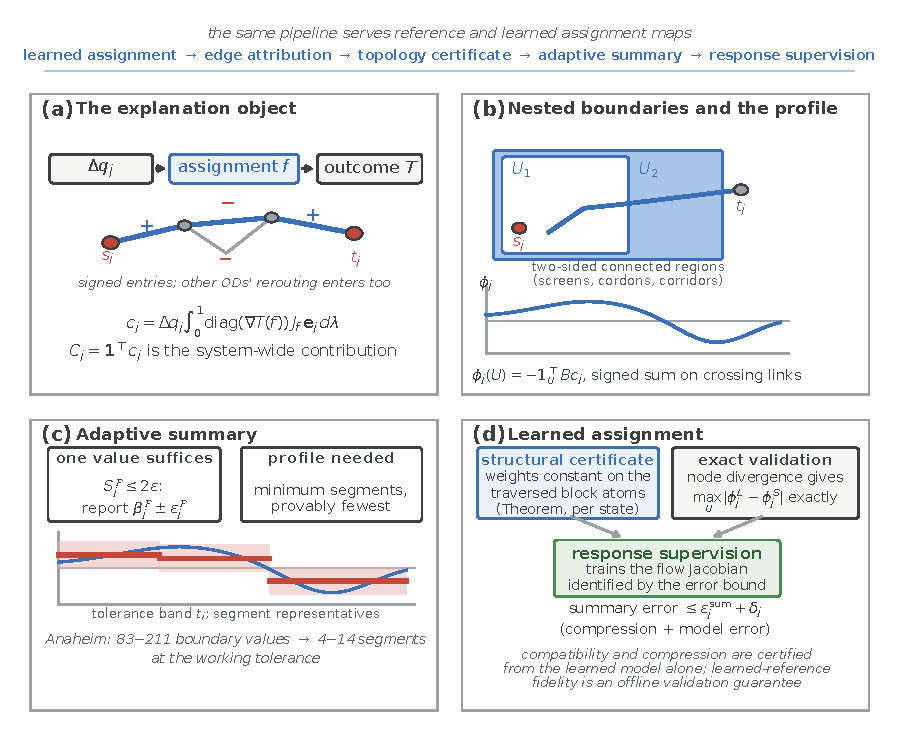
\includegraphics[width=0.90\linewidth]{../figures/fig0_pipeline_v112.pdf}
\caption{The paper as one pipeline. (a)~An OD demand change is
propagated through an assignment map --- a reference SUE model or a
conservative learned surrogate --- and weighted by the outcome's
marginal weights, giving the signed edge-attribution column $c_j$;
rerouting of other ODs enters the same column. (b)~Nested two-sided
connected boundaries turn the column into the boundary-attribution
profile $\phi_j(U)$. (c)~At a prescribed tolerance the profile is
reported either by one transferable value (when its certified range is
small enough) or by the minimum-segment summary, each value carrying
its explicit error. (d)~For learned assignment, the topology theorem
supplies the structural certificate, node divergence validates the
learned column against a reference exactly, and response supervision
trains the discrepancy the error bound identifies; the reported summary
carries a total budget of compression plus model error. Compatibility
and compression are certified from the learned model alone;
learned-reference fidelity is an offline validation guarantee.}\label{fig:pipeline}
\end{figure}

\paragraph{Contributions.}
This paper makes one overarching contribution: it turns the spatial
attribution of OD demand effects from an arbitrary boundary aggregation
into a mathematically controlled representation for both reference and
learned traffic assignment. First, we characterize exactly when a
boundary-attribution profile admits one transferable value. For
two-sided connected regions, this occurs for every conservative
response if and only if the marginal outcome weights agree on the
biconnected edge blocks and bridges traversed by the queried OD path;
weights outside that path are unrestricted --- the principal structural
result of the paper. Second, when one value is insufficient, node
divergence yields the exact profile range and the coarsest ordered
summary satisfying a prescribed approximation tolerance, together with
separate model and compression errors --- the operational and
reporting consequence of that result. Third, the same error
representation identifies demand-to-flow response mismatch as the
trainable source of learned explanation error and leads to response
supervision, which improves spatial attribution on both Sioux Falls and
Anaheim without sacrificing flow accuracy --- its learning consequence.

\section{Related work}\label{sec:related}
\paragraph{Attribution and cost allocation.}
Our edge-level object is input-specific conductance
\citep{dhamdhere2019important,lundstrom2022rigorous}: demand is the input,
link flow is an intermediate variable, and the traffic outcome is the output.
Its sum over links gives the integrated-gradient contribution of an OD, and
continuous marginal cost allocation underlies Aumann--Shapley sharing
\citep{aumann1974values,billera1978internal}. In transportation
applications, attribution typically explains a prediction model by ranking
its input features \citep{sariyer2024leveraging,guo2024towards}, whereas
the object attributed here is a link flow that must satisfy node balance.
Existing scalar attribution methods do not characterize how a fixed OD
contribution changes across physical network boundaries; that additional
property is what we analyze.

\paragraph{Conserved attribution flows on graphs.}
Graph-based explanation methods construct attribution flows with
boundary-consistency or conservation properties on directed acyclic
graphs: Shapley Flow makes edge attributions consistent across
different choices of explanatory boundary, and the recursive Shapley
value recursively constructs edge-attribution flows that conserve at
internal nodes \citep{wang2021shapleyflow,singal2021rsv}. Those works
design new attribution rules satisfying such axioms on computational or
causal graphs; the present problem instead asks when an already
specified traffic-outcome attribution is boundary-consistent on a
cyclic physical network, uniformly over flow-conserving responses.

\paragraph{Traffic sensitivity and learned assignment.}
Equilibrium sensitivity analysis studies demand-to-flow derivatives and
their aggregation
\citep{tobin1988sensitivity,yang2005sensitivity,josefsson2007sensitivity,patriksson2003aggregated}.
Learned assignment maps, implicit optimization layers, and logit
equilibrium metamodels make such derivatives available to explanations
\citep{liu2023endtoend,amos2017optnet,lassen2025learning}; training on
derivative targets is Sobolev training
\citep{czarnecki2017sobolev,yuan2022sobolev}; fully differentiable
formulations propagate these gradients end to end
\citep{li2026differentiable,seo2026differentiable}, graph-attention
surrogates embed node-based flow conservation in the training loss
\citep{liu2024heterogeneous,liu2025multiclass}, and expressivity and
learning guarantees for end-to-end user-equilibrium models are
established in \citet{liu2025endtoend}. These studies primarily
evaluate flows, efficiency and conservation; physical OD tracking
through assignment and cordon counts concerns commodity flows
\citep{sheffi1985urban,vanzuylen1980most,bar2002origin}. None
quantify whether OD-indexed spatial explanations are transferable or
how their boundary error should be controlled; the present work
supplies both.

\paragraph{Conservation and graph structure.}
Physics-informed losses and conservative architectures constrain physical
outputs \citep{raissi2019physics,shi2021physics,richterpowell2022neural};
projections can enforce constraints exactly \citep{valente2025physics,baez2024guaranteeing}.
We examine their transfer to flow and outcome attributions; for
approximate conservation, derivative bounds of Landau--Kolmogorov type
are classical \citep{shadrin2014landau}, and
Appendix~\ref{app:approx} transfers such control to attribution
residuals. The relevant
circulation space and its decomposition into circuit classes are classical
\citep{oxley2011matroid,hopcroft1973algorithm}. Classical block and
circulation results characterize graph structure; they do not
characterize when an outcome-weighted OD response has one transferable
value over a specified family of traffic regions. The new
classification couples the classical decomposition to queried OD
directions and their transitive equality constraints.

\section{Boundary attribution of OD demand effects}\label{sec:objects}
\subsection{Edge attribution and the spatial aggregation question}
Let $\mathcal G=(V,E)$ be connected, with incidence matrix
$B\in\{-1,0,1\}^{n\times m}$ (negative at a link's tail), OD vectors
$\mu_j=e_{t_j}-e_{s_j}$, $s_j\ne t_j$, and $M=[\mu_1,\ldots,\mu_K]$.
Reciprocal and parallel arcs remain distinct edges when orientations are
forgotten. Let $f:\Omega\subset\R^K\to\R^m$ map demands to flows on an
open demand domain $\Omega$, and
$T:\R^m\to\R$ be a specified edgewise outcome. Assume both maps are $C^1$
on open neighborhoods of the relevant paths. The construction reads as
follows: a demand change is first propagated to link-flow responses,
then weighted by the marginal contribution of each link to the selected
outcome; summing over all links gives the OD's system contribution, and
summing with boundary orientation gives its signed boundary attribution.
With $\Delta q=q^1-q^0$ and
$\gamma(\lambda)=q^0+\lambda\Delta q$, define
\begin{align}
g_j&=\Delta q_j\int_0^1 J_f(\gamma(\lambda))\mathbf e_j\,d\lambda,
\label{eq:Gdef}\\
c_j&=\Delta q_j\int_0^1 D_\lambda J_f(\gamma(\lambda))\mathbf e_j\,d\lambda,
\quad D_\lambda=\operatorname{diag}(\nabla T(f(\gamma(\lambda)))),
\label{eq:Cdef}\\
C_j&=\mathbf1^\top c_j,\qquad
\sum_j C_j=T(f(q^1))-T(f(q^0)).\label{eq:Cscalar}
\end{align}
The vector $g_j$ attributes flow changes; $c_j$ resolves the outcome
contribution through links; $C_j$ is its scalar OD contribution. Both
vectors are signed system sensitivities, including other ODs' route
adjustments, rather than physical commodity flows. Entry $c_{e,j}$ is
input-specific conductance through link $e$
\citep{dhamdhere2019important}.\label{sec:whyC}

If $Bf(q)=Mq$, differentiation and integration give
\begin{equation}
BJ_f(q)=M,\qquad Bg_j=\mu_j\Delta q_j.\label{eq:anchorchain}
\end{equation}
The same conclusion holds for $Bf(q)=Mq+b$ with constant background demand
balance $b$. Outcome attribution is \emph{OD cut consistent} when
$Bc_j=\beta_j\mu_j$ for some $\beta_j\in\R$.
The scale $\beta_j$ is a boundary value, generally different from $C_j$:
on two series links with unit weights, $C_j=2\Delta q_j$ but
$\beta_j=\Delta q_j$. Outcome weighting is what makes cut consistency a
genuine restriction: on two series links, a conservative unit response
$(1,1)$ with weights $(w_1,w_2)$ balances at the intermediate node only
if $w_1=w_2$, although the response itself conserves exactly.

For $s_j\in U\subseteq V\setminus\{t_j\}$, write $b_j=Bc_j$ and define
the boundary attribution $\phi_j(U)=-\mathbf1_U^\top b_j$. Any two
separating sets satisfy
\begin{equation}
\phi_j(U')-\phi_j(U)
=-\sum_{v\in U'\setminus U}b_{jv}
+\sum_{v\in U\setminus U'}b_{jv};
\label{eq:cutdiff}
\end{equation}
for nested sets $U\subseteq U'$ the second term vanishes, leaving
$\phi_j(U')-\phi_j(U)=-\sum_{v\in U'\setminus U}b_{jv}$.
The difference between two boundaries is thus the enclosed imbalance,
with incoming and outgoing regions entering with opposite signs.
For a separable outcome $T(F)=\sum_e g_e(F_e)$, the attribution itself
also has a direct reading. With $\delta^+(U)$ and $\delta^-(U)$ the
arcs leaving and entering $U$,
\begin{equation}
H_U(F)=\sum_{e\in\delta^+(U)}g_e(F_e)-\sum_{e\in\delta^-(U)}g_e(F_e),
\qquad
\phi_j(U)=\operatorname{IG}_j[\,H_U\circ f\,],
\label{eq:hboundary}
\end{equation}
because each entry $c_{e,j}$ of Eq.~\eqref{eq:Cdef} is the
integrated gradient of the scalar outcome $g_e\circ f$, and the
incidence signs turn $-\mathbf 1_U^\top b_j$ into the
signed boundary sum of $H_U$. For TSTT, $\phi_j(U)$ therefore
attributes the demand change to the excess of the total travel cost on
the region's outgoing arcs over that on its incoming arcs: a
boundary-related outcome in its own right, neither the region's
internal cost nor a vehicle count.
\begin{uproposition}[cut-consistency equivalence]\label{par:cutequiv}
OD cut consistency holds exactly when every separating cut has one common
signed value $\phi_j(U)=\beta_j$.
\end{uproposition}
Indeed, balance implies this identity. Conversely, comparing $\{s_j\}$
with $\{s_j,v\}$ forces zero divergence at every interior node; the two
endpoint entries are then opposite because incidence columns sum to zero.
The three spatial summaries of one attribution --- the system-wide value
$C_j=\sum_ec_{e,j}$, attribution $\sum_{e\in E_R}c_{e,j}$ on a road set
$E_R$ specified before aggregation, and the boundary value $\phi_j(U)$
--- answer the three questions of Figure~\ref{fig:pipeline}(a): how
much, where on specified roads, and what signed aggregation on a
specified boundary.

The road partition is part of the attribution object: subdivision changes
which crossing-link costs a boundary includes (Example~\ref{ex:subdivision}).

Throughout, $\mathcal U_j^{\mathrm{all}}$ contains all sets separating
$s_j$ from $t_j$; $\mathcal U_j^{\mathrm{conn}}$ restricts both induced sides
to be connected in the underlying undirected network; and
$\mathcal U_j^{\mathrm{geo}}$ is a specified finite family of straight
screenline regions, filtered for two-sided connectivity.
The unrestricted extrema below are closed-form exact values. Sioux Falls
connected extrema use complete enumeration. Geometric extrema and Anaheim's
selected connected-region ranges are exact only over their stated finite
families, and do not determine extrema over all connected regions.

\subsection{Boundary families, response classes, and explanation accuracy}\label{sec:levels}\label{sec:hierarchy}
A common boundary value is a property of two objects at once: which
boundaries are allowed, and which demand responses are quantified over.
We therefore state the transferability questions along these two axes.
\emph{Boundary families}: all separating regions
$\mathcal U_j^{\mathrm{all}}$; two-sided connected regions
$\mathcal U_j^{\mathrm{conn}}$; or a prescribed finite family such as a
screenline set. \emph{Response classes}: every conservative response at
fixed weights; the path-feasible response envelope of one assignment model;
or a single realized attribution column. The graph-topological
classification of Section~\ref{sec:classification} covers the first two
families under all conservative responses; prescribed finite families
admit an exact linear-algebraic test of the same universal kind
(Proposition~\ref{prop:familycriterion} below), and model envelopes
substitute for the conservative class inside any of them.
Four levels result, ordered by what varies. The \emph{structural}
level asks whether one value is guaranteed for all flow-conserving
responses and is answered by the topological condition of
Section~\ref{sec:classification}; the \emph{model-specific} level asks
the same for the path-feasible response envelope of one assignment
model and is answered by the linear-algebraic test of
Proposition~\ref{prop:familycriterion}; the \emph{realized} level asks
how much the boundaries of one attribution column differ and is
answered by the exact range and profile of
Section~\ref{sec:stability}; and the \emph{learned-reference} level
quantifies the distance between two realized columns, reported
separately from the consistency properties
(Section~\ref{sec:boundarylearning}).

\begin{proposition}[exact family criterion]\label{prop:familycriterion}
Fix a query $j$, a nonempty boundary family
$\mathcal F\subseteq\mathcal U_j^{\mathrm{all}}$, and an affine class of
edge responses $x=x_j^{\mathrm{ref}}+\mathcal S$ with basis $N_{\mathcal S}$
($\mathcal S=\ker B$ recovers all conservative responses). Let
$A_{\mathcal F}=[-\mathbf 1_U^\top B]_{U\in\mathcal F}$ stack the oriented
attribution functionals. All responses in the class give one common summary
$\alpha_j$ on $\mathcal F$ --- that is,
$-\mathbf 1_U^\top BDx=\alpha_j$ for every $U\in\mathcal F$ and every
$x\in x_j^{\mathrm{ref}}+\mathcal S$ --- if and only if
\begin{equation}
A_{\mathcal F}DN_{\mathcal S}=0
\qquad\text{and}\qquad
A_{\mathcal F}Dx_j^{\mathrm{ref}}\in\operatorname{span}\{\mathbf 1\},
\label{eq:familycriterion}
\end{equation}
in which case $\alpha_j$ is the common entry of $A_{\mathcal F}Dx_j^{\mathrm{ref}}$.
\end{proposition}
Substituting $x=x_j^{\mathrm{ref}}+N_{\mathcal S}z$ makes the attribution
affine in $z$; the identity holds for every $z$ exactly when the
$z$-coefficient block $A_{\mathcal F}DN_{\mathcal S}$ vanishes and the
constant block has constant rows. On the full separating family the
criterion reproduces the classification theorems, which characterize
when \eqref{eq:familycriterion} holds for every weight profile without
enumerating $\mathcal F$; on a prescribed screenline set it is the exact
universal test, computable from one sparse product per family member.
For a fixed assignment model, the envelope
$x_j^{\mathrm{ref}}+\mathcal S$ collects the path-feasible responses
that the fixed path sets can express; the tests are then sufficient
for the actual assignment map, and necessity for a specified
equilibrium map would require a separate attainability argument, which
we do not claim. On Sioux Falls, whose full-background fixed-path
model allows path exchanges spanning the complete circulation space
($T_{\mathrm{swap}}=\Delta\ker A_{\mathrm{OD}}$ of dimension $m-n+1$),
the path-exchange envelope coincides with the affine space of
conservative responses: for this path-feasible response envelope, the
model-specific criterion coincides with the unrestricted
conservative-response criterion, so the universal condition is tight
rather than conservative for that path structure; restricted path
systems separate the two levels (Appendix~\ref{supp:networks},
Table~\ref{tab:levelsdiag}).
A realized attribution can balance without satisfying the universal
conditions; pointwise balance along a demand path implies integrated
balance, and the converse can fail through cancellation.
Appendix~\ref{supp:criteria} collects these examples and the
directionality conditions under which weaker balance notions coincide
with the classified property.

\section{Topological conditions for transferable spatial attribution}\label{sec:classification}
Take the block-cut tree of the underlying undirected multigraph.
Its non-bridge blocks, together with each bridge as a singleton,
are the \emph{block atoms}. They are the classical graphic-matroid circuit
classes, with each bridge retained separately. The \emph{OD block path}
$\mathcal P(s,t)$ is the atom sequence on the unique block-cut-tree path
between the OD endpoints. For several queries, merge all atoms traversed
by each $\mathcal P_j=\mathcal P(s_j,t_j)$ and take the transitive closure.
The resulting edge sets $\bar E_1,\ldots,\bar E_{K'}$ are the
\emph{OD-compatibility classes}; atoms on no queried path remain separate.

\begin{figure}[pos=t]
\centering
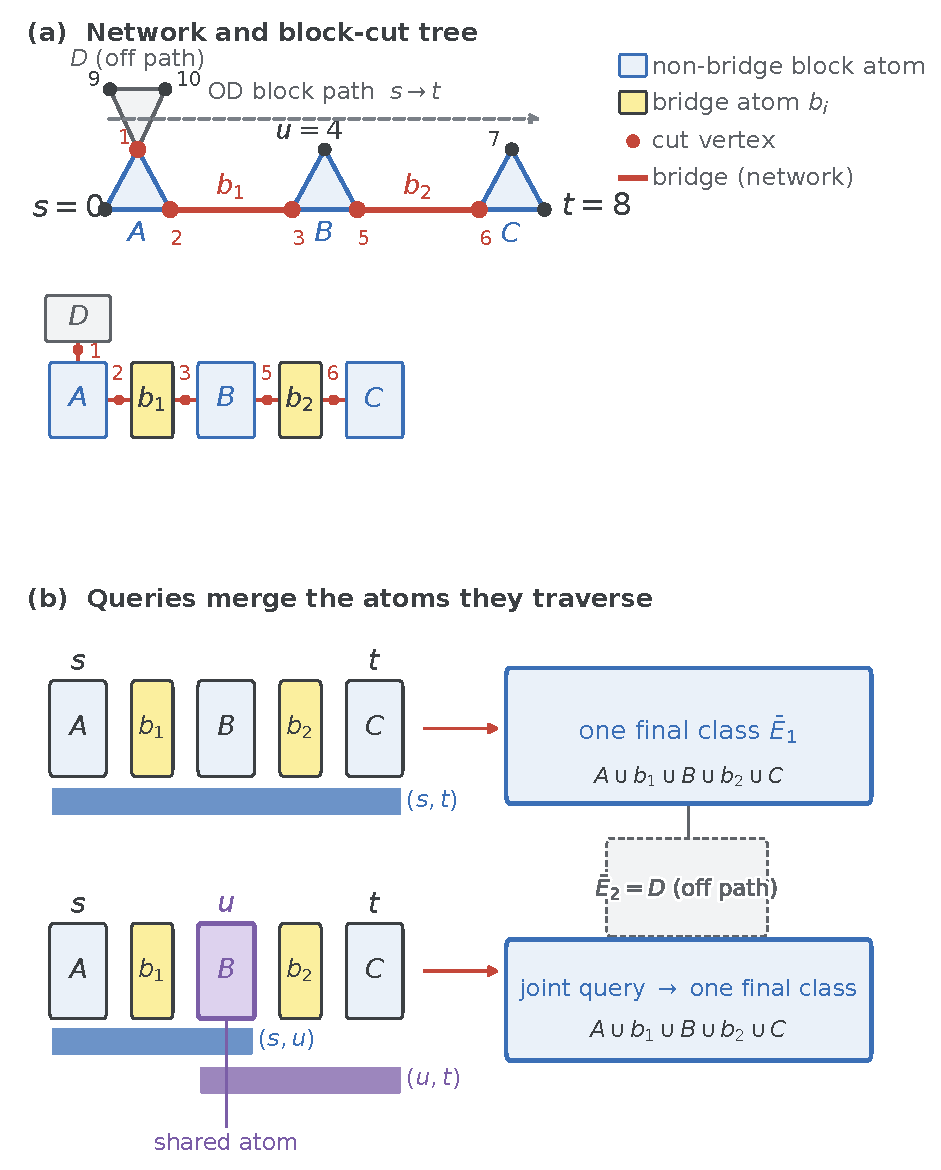
\includegraphics[width=0.74\linewidth]{../figures/fig1_block_cut_v108.pdf}
\caption{(a)~A two-bridge network with its block-cut tree: non-bridge
block atoms $A,B,C,D$ and bridge atoms $b_1,b_2$ joined at shared cut
vertices; the queried OD path runs $s\to t$ and the pendant atom $D$
hangs off the path. (b)~OD queries merge the atoms they traverse: the
single query $(s,t)$ merges $A\cup b_1\cup B\cup b_2\cup C$ into one
class while $D$ stays separate; two queries $(s,u)$ and $(u,t)$ sharing
only atom $B$ merge the same full chain transitively. In the
connected-region example below, atom $D$ carries heterogeneous weights
$3,4,5$ --- invisible to the queried connected boundaries but violating
unrestricted transferability; the unrestricted-family counterpart with
uniform pendant weights appears as Example~B in
Appendix~\ref{app:classificationproof}.}\label{fig:blockcut}
\end{figure}

\subsection{Main result: two-sided connected traffic regions}\label{sec:connectedmain}
Traffic analysis typically aggregates on screenlines, cordons and regional
boundaries whose two sides are each spatially connected. The main theorem
shows that this restriction strictly localizes the condition for a
common boundary attribution to the queried OD block path; the magnitude
of the resulting freedom is topology- and query-dependent. Let
\[
\mathcal U^{\mathrm{conn}}_{st}=\{U\subset V:s\in U,\ t\notin U,
\ \mathcal G[U]\text{ and }\mathcal G[V\setminus U]\text{ are connected}\},
\]
where connectivity uses the underlying undirected multigraph. These are
separating bonds: both sides of the boundary form connected regions.

\medskip
\noindent\fbox{\parbox{\dimexpr\linewidth-2\fboxsep-2\fboxrule\relax}{%
\textbf{Main implication.} For two-sided connected traffic regions,
transferable OD boundary explanations require uniform marginal weighting
only along the block atoms traversed by the queried OD paths.
Heterogeneity elsewhere in the network is immaterial to this guarantee.}}
\medskip

\begin{theorem}[two-sided connected-region classification]\label{thm:connectedclassification}
For a connected loopless multigraph, $\mu=e_t-e_s$, and
$D=\operatorname{diag}(w)$, the property
\begin{equation}
\exists\alpha\in\R\quad\forall x\text{ with }Bx=\mu\quad
\forall U\in\mathcal U^{\mathrm{conn}}_{st}:
-\mathbf1_U^\top BDx=\alpha
\label{eq:connectedclassification}
\end{equation}
holds if and only if every edge in the atoms of $\mathcal P(s,t)$ has
one common weight $\alpha$. Weights of edges outside those atoms are
arbitrary, even within an off-path block atom.
\end{theorem}
The proof in Appendix~\ref{app:connectedproof} uses connected prefix and
suffix regions within each traversed atom. Each admissible boundary
crosses edges in just one such atom, which explains why off-path
heterogeneity is invisible to this region family. This is a universal
fixed-weight statement; agreement for one realized response need not
imply its conditions.

\begin{corollary}[several queries on connected regions]\label{cor:connectedmulti}
At one shared weight vector, Eq.~\eqref{eq:connectedclassification} holds
for all queried ODs if and only if edges in each group of atoms joined
by the queried block paths have one common weight. An atom on no queried
path has no weight restriction, including no within-atom restriction.
\end{corollary}
Thus restricting attention to connected traffic regions permits additional
outcome heterogeneity. It changes the compatibility classification,
while the unrestricted extrema and error formulas of
Section~\ref{sec:stability} retain their own stated boundary family.

\subsection{Design implications}\label{sec:design}
The theorem gives three design freedoms, each checkable before any model
is fitted.
\paragraph{Query design.}
Only the atoms traversed by the queried OD paths enter the condition, and
adding queries merges atoms transitively through shared blocks. On
Figure~\ref{fig:blockcut} ($s=0$, $u=4$, $t=8$, linear outcome
$T_w(F)=w^\top F$), the query $(s,u)$ joins $A,b_1,B$ while $b_2$, $C$
and $D$ keep their own constants; adding $(u,t)$ joins the remaining
chain through the shared atom $B$; adjusting only $b_2$ and $C$ then
restores a common summary for both queries while the unrelated atom $D$
keeps weight $3$. Appendix~\ref{app:classificationproof} tabulates the
three stages with exact profile ranges.
\paragraph{A constructive distinction on Figure~\ref{fig:blockcut}
(Example~A).}
Keep weights $1$ on $A,b_1,B$, weights $2$ on $b_2,C$, but set the three
off-path $D$ weights to $3,4,5$. The first query $(s,u)$ admits common
boundary value $1$ on every two-sided connected region for every conservative
response. The second query $(u,t)$ initially has connected boundary values
spanning $[1,2]$ and requires a segmented profile. Changing only
$b_2,C$ to weight $1$ makes both queries compatible on connected
regions, while $D$ remains internally heterogeneous --- permissible
for connected transferability, since no queried connected boundary
sees inside $D$. The model-specific diagnosis of
Table~\ref{tab:levelsdiag} verifies exactly this post-merge
configuration in its synthetic row. The unrestricted theorem makes a
stricter demand on the same network; that counterpart, with uniform
pendant weights, is Example~B below.

\paragraph{Outcome design.}
\begin{corollary}[linear outcome functionals]\label{cor:linear}
Let $f\in C^1$ be exactly conservative on an open neighborhood of the
attribution path, and let $T(F)=a^\top F$ be a linear functional of
realized flows. Then $\nabla T\equiv a$, so structural cut consistency
over the unrestricted separating family holds if and only if $a$ is
constant on the compatibility classes, with common cut value
$\beta_j=\Delta q_j\,a|_{\bigcup\mathcal{P}_j}$; over two-sided
connected regions the weaker condition of
Theorem~\ref{thm:connectedclassification} applies instead --- $a$
constant on the block atoms traversed by the queried OD paths, with no
constraint on off-path atoms. Both are conditions on the outcome
definition alone, checkable by inspection before any model is trained,
and the pointwise classification holds at every $\lambda$.
\end{corollary}
Nonlinear compatible outcomes also exist: if
$T(F)=\Phi(\sum_{e\in\bar E_1}F_e,\ldots,\sum_{e\in\bar E_{K'}}F_e)$,
its gradient is class-constant at every flow. More familiar traffic outcomes
require equality of their actual marginal weights. The Beckmann potential
has weights $t_e(F_e)$; total system travel time (TSTT) has weights
$t_e(F_e)+F_et'_e(F_e)$; a separable index $\sum_e g_e(F_e)$ has
weights $g'_e(F_e)$. Heterogeneous link parameters and congestion typically
violate these equalities. A single-link outcome has a nonzero common boundary value
only when the queried OD block path is precisely that singleton bridge.
\paragraph{Region-family design.}
The admissible family is part of the attribution question, and the theorem
quantifies what each choice costs: the connected family ignores off-path
heterogeneity, the unrestricted family does not, and a prescribed finite
family such as a screenline set admits the exact universal test of
Proposition~\ref{prop:familycriterion} in place of a graph-topological
classification.
On public road networks the size of that freedom is itself measurable
from topology alone, and it is largest for corridor-type and
articulation-adjacent queries and smaller in large biconnected cores.
Across every positive-demand OD pair, the share of edges the connected
condition constrains --- against $100\%$ for the unrestricted condition
--- has median $100\%$ on Sioux Falls (one atom), $95.4\%$ on Anaheim,
$95.3\%$ on Winnipeg and $89.1\%$ on Eastern-Massachusetts. The
distribution is tightly concentrated on the first three networks
(Anaheim $10$--$90\%$ quantiles $95.4$--$96.1\%$), whereas
Eastern-Massachusetts carries a genuine peripheral tail: $2.2\%$ of OD
pairs constrain fewer than $75\%$ of edges, down to $0.8\%$ for OD
pairs localized in a single peripheral block (Appendix~\ref{supp:networks},
Table~\ref{tab:topologydist}). Where the release is small, the
realized summaries of Section~\ref{sec:stability}, not the structural
classification, carry the reporting.

\subsection{A stronger criterion for all separating sets}\label{sec:allsets}
When every separating set --- regular or irregular --- must share one
boundary value, the condition tightens and reaches beyond the queried paths.

\Needspace{15\baselineskip}
\begin{theorem}[single-OD classification, static form]\label{thm:t3cpmain}
Let $\mathcal{G}$ be a connected multigraph with one OD pair $(s,t)$,
\textbf{$s\neq t$}, let
$w\in\R^m$, and let $D=\operatorname{diag}(w)$. The
\emph{response-independent OD cut consistency property}
\begin{equation}
\exists\,\alpha\in\R:\qquad BDx=\alpha\,\mu
\quad\text{for every }x\in\R^m\text{ with }Bx=\mu,
\label{eq:t3prop}
\end{equation}
with the scale $\alpha$ independent of the response $x$, holds
\textbf{if and only if}
\begin{enumerate}[(i)]
\item $w$ is constant within every non-bridge atom; and
\item all atoms on the $s$--$t$ block path $\mathcal{P}(s,t)$ share
one common value.
\end{enumerate}
In that case every conservative response induces the same boundary vector:
$BDx=w^*\mu$ for every $x$ with $Bx=\mu$, where
$w^*:=w|_{\bigcup\mathcal{P}(s,t)}$ is the common value of (ii) and
$\alpha=w^*$ is the scale in \eqref{eq:t3prop}.
\end{theorem}

Condition (i) concerns every atom, including those off the OD path. Their
constants may differ; only the traversed atoms must share the scale $w^*$.
Off-path atoms are constrained because a signed circulation can
be added to any conservative response, and heterogeneous weights can turn
it into node divergence. Connected regions change this conclusion, as
Theorem~\ref{thm:connectedclassification} shows. The proof adds a virtual
edge from $t$ back to $s$
(Appendix~\ref{app:classificationproof}): conservative OD responses then
become circulations on the extended graph, so the boundary vector is
response-independent exactly when diagonal weighting preserves the
circulation space --- equivalently, when every weighted cycle has zero
node divergence --- which forces equal weights within each block atom
and one shared weight along the atoms the OD block path connects.

\begin{theorem}[multi-OD classification, static form at a shared
realized flow state]\label{thm:t3cm}
Let $\mathcal{G}$ be connected, let each OD pair satisfy $s_j\ne t_j$,
and let $w\in\R^m$, $D=\operatorname{diag}(w)$. The
response-independent OD cut consistency property \eqref{eq:t3prop}
--- for each queried $j$, some $\alpha_j\in\R$ with
$BDx=\alpha_j\mu_j$ for every $x$ with $Bx=\mu_j$ --- holds
simultaneously for the queried ODs \textbf{if and only if} $w$ is
constant on each OD-compatibility class $\bar{E}_k$.
\end{theorem}

The classification concerns all signed responses compatible with vehicle
conservation; an equilibrium model generally realizes only a subset of
these responses (Appendix~\ref{app:membership}).
All queries use the same realized weight vector. Queries with $\Delta q_j=0$
have zero attribution columns and need not enter the closure. Requiring all
ordered pairs of distinct vertices collapses the classes to one per
connected component (Corollary~\ref{cor:allod}).

\subsection{Pathwise attribution and certificates for learned assignment}\label{sec:pathwise}
\begin{corollary}[path form: endpoint implication]\label{cor:path}
Let $f\in C^1$ be conservative on an open set, $T\in C^1$,
$\gamma(\lambda)=q^0+\lambda\Delta q$ the straight-line path with $\Delta q\ne0$, and
$w(\lambda)=\nabla T(f(\gamma(\lambda)))$, $D_\lambda=\operatorname{diag}(w(\lambda))$, shared by
all participating ODs. If the equivalent conditions of
Theorems~\ref{thm:t3cpmain} and~\ref{thm:t3cm} hold at $w(\lambda)$ for
every $\lambda\in[0,1]$, then, for every participating $j$
simultaneously,
\[
Bc_j=\beta_j\,\mu_j
\]
holds with
\[
\beta_j=\Delta q_j\int_0^1 w^*_{k(j)}(\lambda)\,d\lambda,
\]
where $w^*_{k(j)}$
is the common value on the compatibility class $k(j)$ containing the
atoms of $\mathcal{P}_j$.
\end{corollary}

The specified edgewise outcome and the network representation are both
part of the object. On two series links, an outcome whose marginal
weights oscillate around unity can integrate to the same balanced column
$(1,1)$ as the linear outcome on one demand segment, yet fail to balance
on another (Example~\ref{ex:cancellation}); subdividing a link leaves
the composite map unchanged but creates interior divergence and even
halves the original cut value at the mixed split
(Example~\ref{ex:subdivision}). Response independence concerns
conservative responses on a fixed network; it does not make the attribution
invariant to road subdivision.

\begin{corollary}[conservative learned assignment]\label{cor:learned}
Let $f^L$ be an exactly conservative learned assignment map on an open
domain. Then its flow-valued integrated gradients inherit OD
conservation, $Bg^L_j=\mu_j\Delta q_j$. Write
$w(\lambda)=\nabla T(f^L(\gamma(\lambda)))$ along the attribution path.
For each $\lambda$, structural cut consistency of the learned
explanations is equivalent to the weight conditions of
Theorems~\ref{thm:t3cpmain} and~\ref{thm:t3cm} at $w(\lambda)$ for the
unrestricted separating family, and to those of
Theorem~\ref{thm:connectedclassification} for two-sided connected
regions. When the unrestricted-family conditions hold at every
$\lambda$, the integrated explanations are realized cut consistent,
$Bc^{L}_j=\beta_j\mu_j$
(Corollary~\ref{cor:path}); when they fail at some $\lambda$, the node
representation of Section~\ref{sec:stability} gives the exact spatial
explanation range of the learned column over the unrestricted family
and its exact maximum boundary disagreement from any reference
assignment, with restricted families scanned through the same node
sums.
\end{corollary}
\begin{proof}
The conservation transfer is Eq.~\eqref{eq:anchorchain} applied to
$f^L$. The pointwise equivalences are the two classification theorems
applied to the fixed weight vector $w(\lambda)$; the integral claim is
Corollary~\ref{cor:path} with
$D_\lambda=\operatorname{diag}(w(\lambda))$; the general-profile bound is
Corollary~\ref{cor:boundaryerror}.
\end{proof}
Conservation of predicted flows is thus the first step of a chain whose
later steps are topological; Section~\ref{sec:pairresults} evaluates the
whole chain empirically.

\FloatBarrier
\section{Adaptive spatial summaries and error guarantees}\label{sec:stability}\label{sec:algorithm}
Procedure~\ref{alg:spatial} summarizes the full pipeline from an OD
demand change to a reported explanation; the subsections that follow
derive each step in turn.

\subsection{Obtaining attribution columns}

\begin{algo}[t]
\caption{From an OD demand change to a reported spatial explanation}\label{alg:spatial}
\small
\textbf{Input:} incidence $B$, query $(s_j,t_j)$, edge attribution $c_j$,
an ordered boundary family $\mathcal F$ with tolerance $\epsilon_j$,
selected regions $U,W$, and optionally a reference column $c'_j$.\\
0. For a single changing OD and separable outcome, obtain $c_j$ from the two endpoint states using Eq.~\eqref{eq:edgeidentity}; for joint changes, input the separately integrated column.\\
1. Compute $b_j=Bc_j$; return its node distribution.\\
2. Return $\phi_j(U)=-\mathbf1_U^\top b_j$ and
$\phi_j(U)-\phi_j(W)=-(\mathbf1_U-\mathbf1_W)^\top b_j$: the
boundary-attribution profile over $\mathcal F$.\\
3. Scan interior nodes to return the extrema in Eq.~\eqref{eq:cutextrema}
and the midpoint and half-range in Eq.~\eqref{eq:familycommon},
and their sets $\{s_j\}\cup\{v\in V\setminus\{s_j,t_j\}:b_{jv}>0\}$ and
$\{s_j\}\cup\{v\in V\setminus\{s_j,t_j\}:b_{jv}<0\}$.\\
4. Summarize: if $\varepsilon_j^{\mathcal F}\le\epsilon_j$ return the common
summary $\beta_j^{\mathcal F}$; otherwise apply
Proposition~\ref{prop:segmented} and return the minimum-segment
summary with each segment's position range, representative value and
worst error ($\le\epsilon_j$ by construction).\\
5. If $c'_j$ is supplied, return $\mathcal K_j(c_j-c'_j)$ as the exact
maximum absolute error over unrestricted separating regions, the family
scan over $\mathcal F$, and, when step 4 produced a summary, the total
budget $\varepsilon^{\mathrm{sum}}_j+\delta_j$ of
Eq.~\eqref{eq:totalbudget}.\\
The incidence product and scan cost $O(|E|+|V|)$ per column; selected-region
sums cost $O(|V|)$; the segmentation is one linear pass over the family.
The same node representation serves all these tasks. The columns must already
have been computed; their reference-attribution cost remains separate.
\end{algo}
For a separable outcome $T(F)=\sum_e g_e(F_e)$, a single changing OD gives
\begin{equation}
c_{e,j}=g_e(F_e^1)-g_e(F_e^0).
\label{eq:edgeidentity}
\end{equation}
Along this demand path, $dF_e/d\lambda=\Delta q_j\partial_jf_e$; the fundamental theorem of calculus applies link by link, including endogenous background rerouting. Two endpoint assignments therefore recover the attribution column without sensitivity integration. The boundary attribution is $H_U(F^1)-H_U(F^0)$.
For jointly changing ODs, endpoint differences determine only the sum of attribution columns. Sensitivity integration in Eq.~\eqref{eq:Cdef} separates the individual OD contributions. Both cases then use the same node representation and spatial aggregation (Procedure~\ref{alg:spatial}) below. After preprocessing, all boundary values for a prescribed screenline family are obtained from one incidence multiplication and a linear scan; numerical verification and same-task timings against endpoint and vectorized alternatives are collected in Appendix~\ref{supp:timing}.
\subsection{Node representation and exact profile ranges}
Once the classes are constructed, structural cut consistency over the
unrestricted family of all separating regions is tested by
\begin{equation}
\eta_{\mathrm{all}}(\lambda)=\max_k\max_{e\in\bar E_k}|w_e(\lambda)-\bar w_k(\lambda)|,
\qquad
\bar w_k=|\bar E_k|^{-1}\sum_{e\in\bar E_k}w_e,
\label{eq:etaall}
\end{equation}
and the joint condition of Theorem~\ref{thm:t3cm} is exactly
$\eta_{\mathrm{all}}=0$. For two-sided connected regions, let
$E_Q=\bigcup_j\bigcup_{A\in\mathcal P_j}A$ collect the edges of all queried
block paths and define
\begin{equation}
\eta_{\mathrm{conn}}(\lambda)=
\max_{k:\,\bar E_k\cap E_Q\neq\varnothing}\;
\max_{e\in\bar E_k}|w_e(\lambda)-\bar w_k(\lambda)|,
\label{eq:etaconn}
\end{equation}
which omits every class on no queried path. By
Corollary~\ref{cor:connectedmulti}, $\eta_{\mathrm{conn}}=0$ is exactly the
connected-region compatibility condition, and off-path atoms may remain
internally heterogeneous, so $\eta_{\mathrm{conn}}=0$ does not imply
$\eta_{\mathrm{all}}=0$. Class construction uses the
block-cut tree and transitive merging; testing a weight vector then needs
one edge scan. No fitted-model derivatives are required for a linear outcome.

For a realized integrated attribution, define
\begin{equation}
d_j=(I-P_{\mu_j})Bc_j,\qquad
P_{\mu_j}=\frac{\mu_j\mu_j^\top}{\norm{\mu_j}_2^2}.
\label{eq:endpointd}
\end{equation}
Endpoint cut consistency over all separating regions holds precisely when
$d_j=0$; only then does
$\mu_j^\top Bc_j/\norm{\mu_j}_2^2$ represent a common cut
value, whatever mechanism produced the balance
(Section~\ref{sec:levels}). For a connected family or another prescribed
finite family, $d_j=0$ is sufficient but not necessary; realized
consistency is then read from the attribution range over that family.

Without a connectivity restriction, each interior node can enter the
separating set independently. Therefore Eq.~\eqref{eq:cutdiff} gives
\begin{equation}
S_j:=\max_U\phi_j(U)-\min_U\phi_j(U)
=\sum_{v\notin\{s_j,t_j\}}|(Bc_j)_v|.
\label{eq:cutspread}
\end{equation}
The extrema themselves have a closed form: writing $b_j=Bc_j$
(Eq.~\eqref{eq:Cdef}), $(x)_+=\max(x,0)$, and summing over interior nodes
$v\notin\{s_j,t_j\}$,
\begin{equation}
\phi_j^{\min}=\phi_j(\{s_j\})-\sum_v(b_{jv})_+,
\qquad
\phi_j^{\max}=\phi_j(\{s_j\})+\sum_v(-b_{jv})_+,
\label{eq:cutextrema}
\end{equation}
since the minimizing set retains exactly the interior nodes with
positive divergence. Subtracting gives, for $I_j=V\setminus\{s_j,t_j\}$,
\begin{equation}
\phi_j(U)-\phi_j^{\min}
=\sum_{v\in I_j\setminus U}(b_{jv})_+
+\sum_{v\in I_j\cap U}(-b_{jv})_+
\quad\text{and}\quad
S_j\le\sqrt{n-2}\,\norm{d_j}_2,
\label{eq:cutgap}
\end{equation}
the first identity being the exact gap to the unrestricted minimum ---
the positive divergence the region omits plus the negative divergence
it contains --- and the second the Cauchy--Schwarz bound (the
projector of Eq.~\eqref{eq:endpointd} changes only the two endpoint
entries). When
$\phi_j(\{s_j\})>0$, the unrestricted family
therefore contains a negative boundary value whenever the interior positive
divergence $\sum_v(b_{jv})_+$ exceeds the origin-cut value: node
imbalance, extremal location, and sign crossing are the same statement.
$S_j=0$ is equivalent to $d_j=0$.
For network regions whose induced subgraphs and complements are both
connected, define $S_j^{\mathrm{conn}}$ by restricting the same extrema to
that family. Then $S_j^{\mathrm{conn}}\le S_j$. We report both
ranges as percentages of the absolute origin-cut value
$|\phi_j(\{s_j\})|$, which remains explicit because the ratio depends
on that denominator (absolute ranges when it is zero). Within each
region family, the four levels above apply with
their family-specific form: the unrestricted column uses
$\eta_{\mathrm{all}}$ and $d_j$, connected families use
$\eta_{\mathrm{conn}}$ and the family's profile range, and a
prescribed finite family $\mathcal F$ uses the exact criterion of
Proposition~\ref{prop:familycriterion}; for
maximum model difference, $\mathcal K_j(e_j)$ is exact and family
scans give the restricted value.

\begin{corollary}[best common boundary value]\label{cor:approxinterchange}
For the unrestricted family, the unique best constant in maximum absolute
boundary error is
\[
\beta_j^\star=\frac{\phi_j^{\max}+\phi_j^{\min}}2
=\frac{(b_j)_{t_j}-(b_j)_{s_j}}2,\qquad
\min_{\beta\in\mathbb R}\max_{U\in\mathcal U_j^{\mathrm{all}}}
|\phi_j(U)-\beta|=\frac{S_j}{2}.
\]
Hence all separating boundary values lie within a prescribed absolute tolerance
$\varepsilon$ of some common value if and only if $S_j\le2\varepsilon$.
\end{corollary}
\begin{proof}
For any constant, its largest error at the two attained extrema is at least
half their difference; their midpoint attains this bound for every boundary value.
Equation~\eqref{eq:cutextrema} and $\mathbf1^\top b_j=0$ give the midpoint formula.
\end{proof}
The coefficient agrees with the endpoint projection in
Eq.~\eqref{eq:endpointd}. It approximates the original boundary values; it does
not change their edge attribution or define a new system contribution.

\subsection{Common values and minimum-segment summaries}\label{sec:segments}
For any nonempty prescribed finite family $\mathcal F$, the same midpoint argument gives
\begin{equation}
\beta_j^{\mathcal F}=\frac{\phi_{j,\max}^{\mathcal F}+\phi_{j,\min}^{\mathcal F}}2,
\qquad \varepsilon_j^{\mathcal F}=\frac{\phi_{j,\max}^{\mathcal F}-\phi_{j,\min}^{\mathcal F}}2,
\qquad |\phi_j(U)-\beta_j^{\mathcal F}|\le\varepsilon_j^{\mathcal F}\quad(U\in\mathcal F).
\label{eq:familycommon}
\end{equation}
Ordered families --- a corridor's nested screenlines, or the regions of
one projection direction --- additionally support piecewise common
summaries. The construction is stated for any ordered family.
\begin{proposition}[minimal contiguous boundary summary]\label{prop:segmented}
Fix an ordered family of boundary values $a_1,\ldots,a_N$ and a
tolerance $\epsilon>0$. Among partitions into contiguous intervals
whose every interval has range at most $2\epsilon$ and does not
strictly mix signs, the longest-feasible-prefix procedure returns one
with the minimum number of intervals. The rule is elementary and
applies to any ordered sequence; its value here is the coupling to the
boundary scan, the node-difference interpretation, and a stated
tolerance --- a single interval reproduces the common summary of
Eq.~\eqref{eq:familycommon}.
\end{proposition}
When a reported family consists of several ordered chains --- the
36-direction geometric family used on Sioux Falls induces 22--35
distinct chains per query --- the procedure is applied within each
chain and the reported count is the sum over chains; the minimality
guarantee is per chain.
\begin{proof}
No feasible first interval can extend past the longest feasible prefix,
so every optimal partition starts with a prefix no longer than the
greedy choice; replacing the first interval of an optimal partition by
the full greedy prefix cannot make the remainder infeasible, and the
same argument applies inductively to the remainder.
\end{proof}
The tolerance is a reporting choice, and the greedy minimality of
Proposition~\ref{prop:segmented} extends from the constant tolerance
to position-dependent tolerances, which control the relative error at
small-magnitude positions.

\begin{corollary}[position-dependent tolerances]\label{cor:mixedtol}
Fix an ordered family $a_1,\ldots,a_N$ and tolerances $t_i\ge0$. Call
an interval $I$ feasible when some representative $\hat a$ satisfies
$|\hat a-a_i|\le t_i$ for all $i\in I$. Then $I$ is feasible if and
only if
\[
\max_{i\in I}(a_i-t_i)\;\le\;\min_{i\in I}(a_i+t_i).
\]
If the no-mixing rule of Proposition~\ref{prop:segmented} is imposed
as an additional reporting requirement, feasibility is inherited by
subintervals, so the longest-feasible-prefix procedure again returns
the minimum number of contiguous segments, and the segment
representative may be taken as the midpoint of the feasibility
intersection.
\end{corollary}
\begin{proof}
The intersection $\bigcap_{i\in I}[a_i-t_i,\,a_i+t_i]$ is nonempty
exactly under the displayed condition, and every subinterval of a
feasible interval retains a nonempty intersection; the exchange
argument of Proposition~\ref{prop:segmented} then applies verbatim.
\end{proof}
The two standard settings used throughout are instances of this
corollary. The recommended \emph{mixed} setting is the mixed
absolute--relative tolerance
$t_i:=\epsilon_{\mathrm{abs}}+\tau|a_i|$ with
$\epsilon_{\mathrm{abs}}$ at $1\%$ of the family maximum and
$\tau=10\%$. The \emph{absolute} setting is the pure
family-scale absolute rule $\epsilon_j=5\%\max_U|\phi_j(U)|$, which
compresses further but permits large relative errors where the profile
is small. On Anaheim, the mixed setting raises the median segment
count only from $10$ to $12$ (per-query ranges $4$--$14$ absolute
against $6$--$17$ mixed) while cutting the worst relative error at
small-magnitude positions from $55\%$ to $28\%$ in the median over
queries ($94\%$ to $45\%$ at worst; Appendix~\ref{supp:tolerance}
reports the full sensitivity).
Every query therefore receives a usable output under either setting,
and both are reported in the summaries below (the learned-assignment
experiments of Section~\ref{sec:pairresults} use the absolute setting).
The reporting rule is stated once and organizes the numerical sections:

\medskip
\noindent\fbox{\parbox{\dimexpr\linewidth-2\fboxsep-2\fboxrule\relax}{%
\textbf{Adaptive reporting rule.} For a specified boundary family,
report the minimax common value $\beta_j^{\mathcal F}$ when its exact
error $\varepsilon_j^{\mathcal F}$ meets the chosen setting's
tolerance; otherwise report the boundary attribution profile itself,
or its minimum contiguous segmentation, in which every boundary value
$a_i$ is reproduced within its tolerance $t_i$ (mixed:
$t_i=\epsilon_{\mathrm{abs}}+\tau|a_i|$, representative from the
per-segment feasibility intersection; absolute:
$t_i\equiv\epsilon_j=5\%\max_U|\phi_j(U)|$, interval midpoint;
Proposition~\ref{prop:segmented}).}}
\medskip

\noindent The absolute pair remains available regardless of the
normalization, and each ordered boundary family is summarized at the
coarsest resolution that meets the prescribed tolerance: the outcome is
either an error-controlled common value or an error-controlled
profile.

\subsection{Exact scanning of predefined straight screenlines}\label{sec:scan}
Fix $D$ directions before evaluating attribution. For each direction, sort nodes by their coordinate projection and group equal projection values; no screenline splits such a group. A candidate position is a gap between adjacent groups. Forward and reverse union--find sweeps record whether each prefix and suffix induces a connected subgraph. This geometry and topology preprocessing is reusable across queries, demand paths and models.
For one attribution column, form $b_j=Bc_j$ (Eq.~\eqref{eq:Cdef}) and prefix sums $P_{j,k}=\sum_{i\leq k}(b_j)_{\pi(i)}$. If $s_j$ lies in the prefix and $t_j$ outside, its attribution is $-P_{j,k}$; for the reverse orientation it is $P_{j,k}$ because $\mathbf1^\top b_j=0$. Retain only endpoint-separating gaps with both sides connected. Scanning these values gives exact attributions and extrema over this prescribed finite screenline family. Preprocessing takes $O(D(|V|\log|V|+|E|\alpha(|V|)))$; after preprocessing, a column takes $O(|E|+D|V|)$ using sparse incidence multiplication. Duplicate regions may be removed without changing extrema.

On Sioux Falls, 36 directions at five-degree intervals give 1642 admissible query--position boundary values across six queries (duplicates across directions retained for all algorithms). On exactly these oriented regions, the prefix scan, a vectorized baseline that precomputes the signed crossing matrix $A_{\mathcal F}$ (one sparse row per oriented region, $+1$ leaving and $-1$ entering) and aggregates every boundary value with one sparse product $A_{\mathcal F}C$, and direct crossing-edge summation all agree to $2.2\times10^{-11}$ TSTT units once the reference columns are available. Appendix~\ref{supp:timing} reports the same-task timings of the three aggregations and the amortization threshold of the precomputed matrix.


\subsection{Certificates and exact error budgets for learned assignment}\label{sec:boundarylearning}
For a query $j$ and any edge vector $h$, define the seminorm
\begin{equation}
\mathcal K_j(h)=\frac12\left(\left|(Bh)_{t_j}-(Bh)_{s_j}\right|
+\sum_{v\notin\{s_j,t_j\}}|(Bh)_v|\right).
\label{eq:boundaryseminorm}
\end{equation}
\begin{corollary}[exact maximum boundary error]\label{cor:boundaryerror}
Let $e_j=c^L_j-c^S_j$ be the difference
between learned and reference attribution columns. Then
\begin{equation}
\max_{U:s_j\in U,\ t_j\notin U}|\phi_j^L(U)-\phi_j^S(U)|
=\mathcal K_j(e_j).\label{eq:exactboundaryerror}
\end{equation}
At a common demand $q$, write
$h_j(q)=D^L(q)J_j^L(q)-D^S(q)J_j^S(q)$.
For any subfamily $\mathcal U_j$ of separating boundaries,
\begin{equation}
\epsilon_j^{\mathcal U}:=\max_{U\in\mathcal U_j}|\phi_j^L(U)-\phi_j^S(U)|
\le |\Delta q_j|\int_0^1\mathcal K_j(h_j(\gamma(\lambda)))\,d\lambda.
\label{eq:localboundarybound}
\end{equation}
\end{corollary}
The proof in Appendix~\ref{app:boundaryerror} applies
Eq.~\eqref{eq:cutextrema} to the error column. Evaluation requires one
incidence multiplication and node scan, without enumerating boundaries.
Connected regions and straight screenlines inherit an upper bound; their
restricted maxima need not equal $\mathcal K_j(e_j)$. The endpoint term
must be retained: the two explanations may each be cut-consistent but
have different common boundary values, which internal imbalance alone misses.

The seminorm evaluates spatial explanation errors directly.
Equation~\eqref{eq:localboundarybound} identifies the weighted response
discrepancy $h_j(q)=D^L(q)J_j^L(q)-D^S(q)J_j^S(q)$ as the direct local
driver of boundary error, and $\mathcal K_j$ defines the corresponding
reference-matching losses, whose complete specifications are collected
in Appendix~\ref{app:learning-objectives}. In the studied assignment
setting the weight-shift component of $h_j$ is small relative to the
response component (Section~\ref{sec:pairresults}), so the unweighted
Jacobian loss is evaluated as a stable proxy for the weighted quantity;
Section~\ref{sec:pairresults} also evaluates the bound chain of
Eq.~\eqref{eq:localboundarybound} directly on the test paths.

\subsection{Total error budget of learned summaries}\label{sec:totalbudget}
Sections~\ref{sec:segments} and~\ref{sec:boundarylearning} control two
errors separately: how far a summary is from the profile it compresses,
and how far a learned profile is from its reference. A reader of a
learned model's explanation uses both at once --- the minimum-segment
summary of the learned boundary values. Write $a_j^L(U)$ and $a_j^S(U)$ for
the learned and reference boundary values on a family $\mathcal F$,
$\hat a_j^L$ for the learned summary constructed at tolerance
$\varepsilon^{\mathrm{sum}}_j$, and
$\delta_j=\max_{U\in\mathcal F}|a_j^L(U)-a_j^S(U)|$.
\begin{corollary}[total explanation error]\label{cor:totalbudget}
\begin{equation}
\max_{U\in\mathcal F}\bigl|\hat a_j^L(U)-a_j^S(U)\bigr|
\le\varepsilon^{\mathrm{sum}}_j+\delta_j,
\qquad
\delta_j\le\mathcal K_j(e_j)\le|\Delta q_j|\int_0^1\mathcal K_j(h_j(\gamma(\lambda)))\,d\lambda.
\label{eq:totalbudget}
\end{equation}
\end{corollary}
\begin{proof}
Triangle inequality for the split
$\hat a_j^L-a_j^S=(\hat a_j^L-a_j^L)+(a_j^L-a_j^S)$; the first term is
bounded by construction ($\le\varepsilon^{\mathrm{sum}}_j$), the second by
Eq.~\eqref{eq:exactboundaryerror} and Eq.~\eqref{eq:localboundarybound}.
\end{proof}
The budget combines the two outputs of the framework --- a
compression and a learned profile --- into the error of the final
reported artifact. It is a posteriori: the integral bound consumes
reference-response information, so Eq.~\eqref{eq:totalbudget}
characterizes the worst boundary error when reference derivatives are
available, not a deployable guarantee computable from the learned model
alone. Section~\ref{sec:pairresults} evaluates all three quantities on
the test paths.

\paragraph{Scope and interpretation.}\label{sec:noninheritance}
The classification fixes four objects before any model is fitted: the
road representation (subdivision changes which crossing-link costs a
boundary includes, Example~\ref{ex:subdivision}); the outcome
definition (its marginal weights are the classified object); the
attribution path in demand space (with several ODs changing jointly,
the per-query columns are path dependent; the total is not); and the
admissible region family. The structural, model-specific, realized and
learned-reference levels answer different questions and are reported
separately (Section~\ref{sec:levels}).

\paragraph{Approximate conservation.}
For a model with residual $r(q)=Bf(q)-Mq-b$ and constant $b$, the
corresponding flow-attribution residual is
\begin{equation}
R_j:=Bg_j-\mu_j\Delta q_j
=\Delta q_j\int_0^1\partial_jr(\gamma(\lambda))\,d\lambda,
\qquad \sum_jR_j=r(q^1)-r(q^0).
\label{eq:residualidentity}
\end{equation}
Small endpoint residuals control the sum, but individual columns can cancel.
Approximate output conservation controls attribution residuals only when
derivative regularity is also available; Appendix~\ref{app:approx} gives
the $C^{1,1}$ conditions, a local bound, sharpness examples and an
extension to weighted attributions. The traffic experiments below use exactly
conservative models, and Appendix~\ref{app:conservation} compares the
exact parameterization against a conservation penalty and an output
projection on identical supervision, showing that a small output
residual need not imply a small attribution residual.

\section{Error-controlled spatial explanations in traffic networks}\label{sec:numerics}
Sioux Falls absolute attributions use benchmark flows in veh/h and time units of $0.01$ h; multiply an attribution by $0.01$ for the hourly vehicle-hour total. Anaheim uses vehicle-minutes per hour. All experiments use the stated fixed-path logit-SUE assignment models and prespecified demand scenarios; shares reported over boundary families are enumeration shares over those families. The adaptive reporting rule of Section~\ref{sec:stability} organizes the experiments: every query either receives one error-controlled common value or an explicit spatial profile. The five studies are presented in reading order --- the absolute explanation first, its generating mechanisms second, and the spatial resolution it requires last; Table~\ref{tab:experimentmap} (Appendix~\ref{supp:networks}) collects their settings.

\subsection{A large-network spatial explanation}\label{sec:anaheim}
The public Anaheim network has 416 nodes, 914 directed links and 1,406 positive OD demands \citep{tnfrc2024transportation}. Six largest demands change jointly from 0.8 to 1.2 times their published values; other demands remain fixed with endogenous route choices. Ten fixed free-flow shortest paths per OD exclude other zone centroids as intermediate nodes (first through node 39). This calculation uses the existing 41-state attribution columns.
To obtain interpretable region locations without requiring coordinates, define network-distance progress $p(v)=[d_s(v)-d_t(v)+d_s(t)]/[2d_s(t)]$, using shortest distances in the underlying undirected network with the smaller free-flow time on parallel roads --- a purely geometric ordering of the family (assignment paths additionally exclude other zone centroids, the progress metric does not). The origin has progress zero and destination progress one. Group tied levels, retain prefixes with two connected induced sides that separate the OD, and orient every region toward the origin. This distance-based family depends on the network and query, before inspecting any attribution. It is a prescribed family, not all connected regions, and it is single-direction: the nested prefixes are totally ordered by progress, so no direction grouping is needed here.

The case asks one transport question: for a prespecified demand change,
where along the origin--destination direction does the signed
crossing-cost response change markedly, and does the variation come
mainly from the study traffic's congestion adjustment or from
background rerouting? Figure~\ref{fig:anaheimprofile} displays the
query with the largest early--late attribution difference, $(25,2)$,
chosen to illustrate the method at its richest variation; the
aggregate statistics come from all six queries
(Table~\ref{tab:anaheimsegments}). The figure shows the boundary
attribution as a function of progress over the complete family with its
reported four-segment summary, and the four-part mechanism
decomposition along the same axis. The profiles of the remaining five
queries stay positive with family ranges spanning roughly one to one
and a half orders of magnitude (largest-to-smallest attribution ratios
12.5--36.9); the complete per-query numbers --- system contributions,
unrestricted and family ranges, region counts and the attributions of
the three prespecified positions --- are collected in
Appendix~\ref{app:anaheimsettings} (Table~\ref{tab:anaheim}), with the
early--late mechanism differences in Table~\ref{tab:anaheimmechanism}.
\begin{figure}[t]\centering
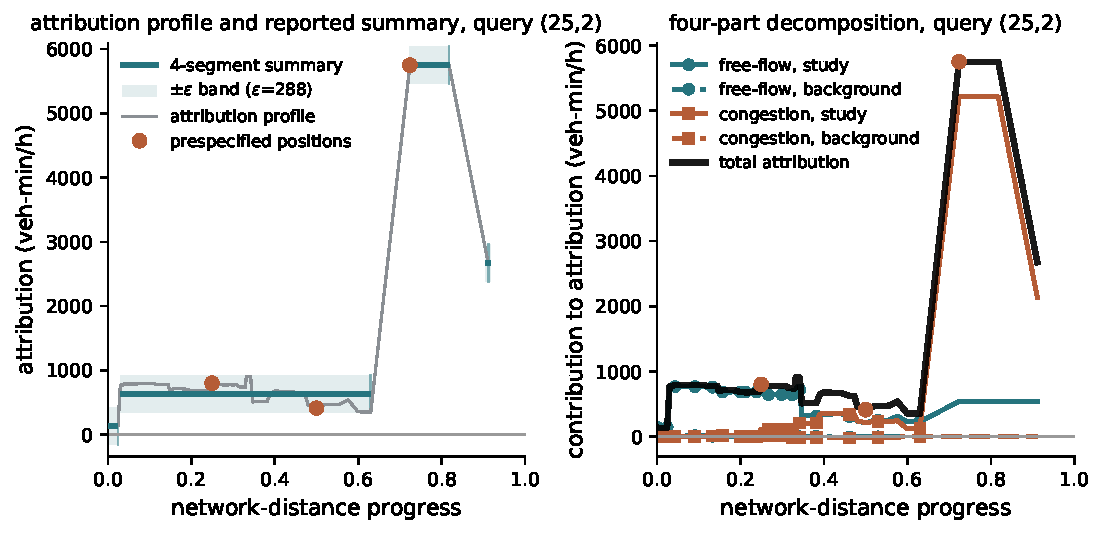
\includegraphics[width=0.99\linewidth]{../figures/fig_v108_anaheim_profile.pdf}
\caption{Anaheim boundary-attribution profile for query $(25,2)$ over
the distance-based family, with its reported summary. Left: attribution
versus network-distance progress along the OD direction (gray curve); the
four-segment minimum summary at the family tolerance (teal step curve
with $\pm\epsilon$ band, $\epsilon=287.6$); ochre dots mark the three
prespecified positions. Right: the four-part mechanism decomposition
(teal: free-flow weights, ochre: congestion weights; solid: study
response, dashed: background); the gray curve is the total
attribution.}\label{fig:anaheimprofile}
\end{figure}

\paragraph{Where the attribution changes.}
The Anaheim TNTP files ship no node coordinates, so the location layer
is reported through the crossing links of each boundary rather than a
map: the three prespecified positions sit at very different network
locations --- the early boundary crosses 34 links with two dominant
contributions, the middle boundary crosses only four links, and the
high plateau isolates the destination neighborhood, where the entire
attribution crosses on the single link $63\!\to\!62$
(Table~\ref{tab:anaheimcrossing}, Appendix~\ref{app:anaheimsettings},
lists the region sizes, crossing links and principal signed
contributions).

\paragraph{Which traffic generates the change.}
The decomposition panel locates the mechanism. At the early position
the attribution is dominated by the free-flow study response ($669.3$
of the total $801.5$, congestion study $111.5$, background below $11$);
at the middle position the two study terms are comparable ($211.5$
free-flow against $212.6$ congestion of the total $412.0$, background
below $11$); at the late position the congestion study term reaches
$5213.7$ while both background terms are below $0.1$ in absolute value:
the rise is congestion adjustment of the study traffic itself on the
destination-side crossing link, not background rerouting. The
decomposition is additive at a common equilibrium state and attributes
the variation to the corresponding response--weight components; the
summary then states, with its error bound, where that variation
changes.

\paragraph{The reported summary.}
Table~\ref{tab:anaheimsegmentsfull} reports the complete four-segment
summary for this query: each segment's position range, the number of
boundary values it summarizes, its representative value, and the actual
worst error within the segment. An origin-side segment covers the six
boundaries nearest the origin at representative value $134.3$ (worst
error $2.5$); one long corridor segment summarizes the 75 boundaries
from progress $0.03$ to $0.63$ at $630.2$ (worst error $279.2$); the
congestion plateau is one segment at $5{,}751.2$ spanning progress
$0.724$--$0.818$; and the destination-side boundary at progress
$0.911$ is reported exactly. Every attribution lies within
$\epsilon=287.6$ of its segment value, the tolerance being $5\%$ of
the family maximum $5{,}751.2$; the reader absorbs four numbers in
place of $84$.
\begin{table}[t]\centering\footnotesize
\caption{The complete reported summary for query $(25,2)$ at the
family tolerance ($\epsilon=287.6$; vehicle-minutes per hour). Each row
is one segment: its progress range, the number of summarized boundary
values, the representative value, and the actual worst error within the
segment (at most $\epsilon$ by construction).}\label{tab:anaheimsegmentsfull}
\setlength{\tabcolsep}{5pt}
\begin{tabular*}{\tblwidth}{@{\extracolsep{\fill}}lrrrr}
\toprule
Segment & Progress range & Boundaries & Representative & Worst error\\
\midrule
1 (origin side) & $0.000$--$0.024$ & 6 & $134.3$ & $2.5$\\
2 (corridor) & $0.030$--$0.630$ & 75 & $630.2$ & $279.2$\\
3 (plateau) & $0.724$--$0.818$ & 2 & $5{,}751.2$ & $0.0$\\
4 (destination) & $0.911$ & 1 & $2{,}673.1$ & $0.0$\\
\bottomrule\end{tabular*}\end{table}
Across the six study queries the compression is uniform:
Table~\ref{tab:anaheimsegments} shows 83--211 boundary values reducing
to 4--14 segments under the absolute tolerance and 6--17 under the
mixed tolerance, with every boundary value within its stated
tolerance by construction; the summary never changes an original
attribution --- it is the same computed profile at its coarsest
resolution that meets the tolerance. The mixed rule controls the
relative error at small attributions (median worst small-value relative
error $54.9\%$ under the absolute rule against $27.8\%$ under the
mixed rule) at a modest segment cost (median 10 against 12).
Aggregation timings and the original construction costs appear in
Appendix~\ref{supp:timing}; the full tolerance sensitivity, including
the mixed absolute--relative rule of Section~\ref{sec:segments},
appears in Appendix~\ref{supp:tolerance}.
\begin{table}[t]\centering\footnotesize
\caption{Reported minimum-segment summaries on Anaheim under the two
tolerance settings of Section~\ref{sec:segments}
(Proposition~\ref{prop:segmented}): absolute ($5\%$ of the largest
attribution magnitude per query) and mixed ($1\%$ absolute floor
plus $10\%$ relative). Worst rel.\ small: worst relative error at
small-magnitude positions (magnitude below one tenth of the family
maximum). Every boundary value in a segment lies
within its tolerance of the representative value; the complete $(25,2)$
absolute-setting segmentation appears in
Table~\ref{tab:anaheimsegmentsfull}.}\label{tab:anaheimsegments}
\setlength{\tabcolsep}{4pt}
\begin{tabular*}{\tblwidth}{@{\extracolsep{\fill}}lrcccc}
\toprule
 & & \multicolumn{2}{c}{Absolute ($5\%$)} & \multicolumn{2}{c}{Mixed ($1\%{+}10\%$)}\\
\cmidrule(lr){3-4}\cmidrule(lr){5-6}
Query & Regions & Segments & Worst rel.\ small (\%) & Segments & Worst rel.\ small (\%)\\
\midrule
$(4,2)$ & 211 & 12 & 94.1 & 13 & 31.9\\
$(1,2)$ & 83 & 8 & 53.6 & 11 & 45.0\\
$(2,4)$ & 211 & 14 & 38.3 & 17 & 3.2\\
$(3,2)$ & 157 & 8 & 56.3 & 11 & 31.4\\
$(25,4)$ & 164 & 13 & 0.0 & 13 & 0.0\\
$(25,2)$ & 84 & 4 & 79.5 & 6 & 24.2\\
\bottomrule\end{tabular*}\end{table}

\subsection{Mechanisms of spatial variation}\label{sec:variation}
We compare three treatments of background traffic: absent, fixed at its
baseline link flows, and responsive through endogenous route choice.
Eight largest published OD demands, all incident to node 10, change
jointly from $0.2$ to $1.6$ times their base values; every study OD has
ten fixed paths. The responsive-background assignment assigns all 528
positive demands (full protocols in Appendix~\ref{supp:fields}).
Uniform weights provide a compatible control. The active-link outcome $T(F)=F_{10\to16}$ preserves the $(10,16)$ direction but permits a response-dependent scale; TSTT produces internal imbalance. Figure~\ref{fig:respfield} illustrates the three patterns on the same realized response: compatible weights give one common boundary value on every boundary, the directional outcome balances along the OD but scales with the response, and TSTT weights generate genuine spatial structure. For its seed-zero TSTT response, expanding $\{10\}$ to $\{10,17\}$ lowers the boundary value from $5.77\times10^4$ to $4.34\times10^4$, approximately $92\%$ of the unrestricted spread. The direct-SUE decrease is $24.80\%$ of its own origin-cut value (Appendix~\ref{supp:accuracy}). Both sides of these regions are connected. Free-flow weights explain $84.7\%$ of the node-17 imbalance: all incident links have free-flow time 2 except $10\leftrightarrow17$ with time 8, giving $[B\operatorname{diag}(t_0)g_j]_{17}=6(g_{10\to17,j}-g_{17\to10,j})$.
\begin{figure}[pos=t]
\centering
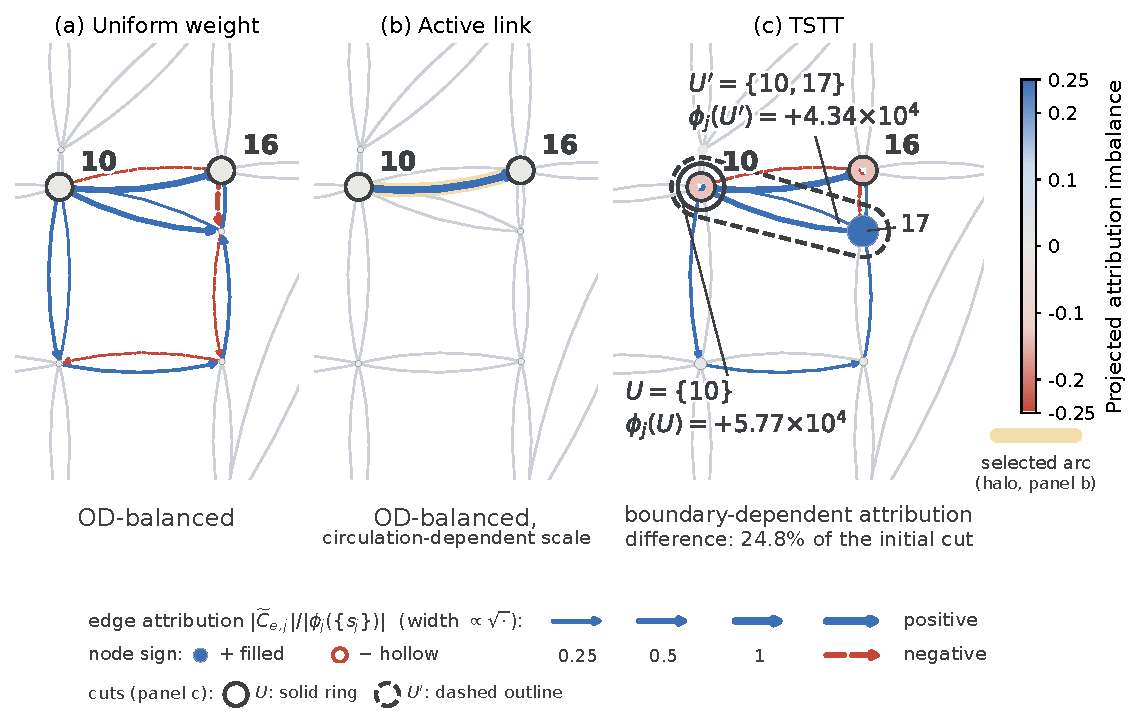
\includegraphics[width=0.9\linewidth]{../figures/fig_resp_field_v109.pdf}
\caption{OD $(10,16)$ endpoint attributions, no-background
assignment, learned
seed $0$. (a) Uniform weights give cut consistency. (b) The signed
TSTT boundary attribution decreases by $24.8\%$ when the boundary expands
from $\{10\}$ to $\{10,17\}$; the active-link outcome --- which
balances in the OD direction but has no response-independent scale ---
is reported in Appendix~\ref{supp:accuracy}. Widths encode attribution
magnitude on the shared square-root scale; node colors show the
projected attribution imbalance $(d_j)_v$ (Eq.~\eqref{eq:endpointd})
divided by the absolute origin-cut value.}
\label{fig:respfield}
\end{figure}

Rerouting produces appreciable spatial variation for every query, and
connected regions retain $60.41$--$76.85\%$ of the unrestricted range
across the full set (complete per-query records for all three
background treatments in Appendix~\ref{supp:additional},
Tables~\ref{tab:bgfull} and~\ref{tab:cutspreadfull}). Normalizations use each setting's own origin boundary value: for
$(17,10)$, the percentage falls from $59.95\%$ under the no-background
treatment to $54.77\%$ under the responsive-background treatment while
the absolute spread rises from 17,607.8 to 123,202.1, approximately
sevenfold.
\paragraph{Response decomposition at common states.}\label{subsec:bgsplit}
Comparing the three background treatments changes both costs and sensitivities. At each common responsive-background state, the mechanism decomposition separates the attribution into study and background response parts, with $BJ_j^{\mathrm{study}}=\mu_j$ and $BJ_j^{\mathrm{bg}}=0$, both weighted by the same total-flow TSTT gradient:
\begin{equation}
c_j^{\mathrm{tot}}=c_j^{\mathrm{study}}+c_j^{\mathrm{bg}}.
\label{eq:bg_attribution}
\end{equation}
At node 15 for $(10,16)$, study and background divergence contributions are $-973.1$ and $49{,}103.4$. Yet on the specified expansion $\{10\}\to\{10,17\}$, the attribution changes only $-3361.1$ ($-1305.0$ study, $-2056.1$ background), or $1.23\%$ of the initial attribution. Large extremal variation can coexist with similar selected boundary values. Component differences add at a fixed region pair; their separate ranges do not add in general.

\paragraph{Free-flow and congestion mechanisms.}\label{subsec:newod}
For BPR costs, $g_e'=t_{0,e}+0.75t_{0,e}(F_e/c_e)^4$. Crossing these two weight terms with the two response terms gives four additive contributions, evaluated at identical states and the same reported boundary:
\[
\phi_j(U_-)=\sum_{a\in\{\mathrm{ff,cong}\}}\sum_{b\in\{\mathrm{study,bg}\}}\phi_j^{a,b},
\qquad \phi_j^{a,b}=-\Delta q_j\int_0^1\mathbf1_{U_-}^{\top}BD_\lambda^aJ_j^b(\lambda)\,d\lambda.
\]
Table~\ref{tab:ffcong} distinguishes the mechanisms behind the sign-crossing queries of Table~\ref{tab:newod}: study congestion dominates $(1,19)$, both congestion terms are negative for $(1,15)$, and background congestion dominates $(7,12)$. The combined free-flow contribution stays positive. The decomposition is additive at a common equilibrium state and identifies the contribution of each response--weight component.
\begin{table}[pos=htbp]
\caption{Four parts of the same boundary attribution at the reported
$U_-$ (responsive-background six-query protocol; TSTT units; identical $41$-point
states, responses, and boundaries as Table~\ref{tab:newod}). Study
includes all six query ODs; background includes the other $522$.
Columns cross free-flow/congestion weights with study/background
responses. Entries are rounded independently.}\label{tab:ffcong}
\small
\begin{tabular*}{\tblwidth}{@{\extracolsep{\fill}}lrrrrr}
\toprule
OD & Free-flow study & Free-flow background & Congestion study & Congestion background & Total\\
\midrule
$(1,19)$ & $-361.3$ & $+759.0$ & $-17{,}357.9$ & $+3{,}458.6$ & $-13{,}501.6$ \\
$(1,15)$ & $+1{,}541.8$ & $+333.8$ & $-6{,}537.4$ & $-3{,}624.2$ & $-8{,}286.0$ \\
$(7,12)$ & $+3{,}897.0$ & $-1{,}311.1$ & $+125.5$ & $-20{,}327.6$ & $-17{,}616.2$ \\
\bottomrule
\end{tabular*}
\end{table}
The sign pattern itself is a spatial property, not a magnitude artifact. Negative attributions occupy $17.8\%$, $2.5\%$ and $7.3\%$ of the 14,477, 15,191 and 16,943 connected regions of the three sign-crossing queries. For $(1,19)$, the connected minimum $-13{,}501.6$ is attained on a 13-node region, whereas a 13-node free-flow neighborhood has attribution $+10{,}756.0$: region size alone does not determine the attribution. At the minimizing boundary, outgoing attributions sum to $7{,}867.3$ and incoming attributions to $21{,}368.8$, so the signed crossing-link attribution is negative while $C_j=50{,}097.7>0$; Figure~\ref{fig:negmech} maps all 26 crossing links. The same contrast appears on the straight screenlines of the prespecified geometric family, whose minimum and maximum attributions for $(1,19)$ have opposite signs under one positive network-wide contribution (Figure~\ref{fig:screenlines}, Appendix~\ref{supp:additional}).
The straight-screenline family uses 36 directions at $5^\circ$ intervals, gaps between node projections, two-sided connectivity and duplicate removal; construction is independent of attribution. It contains 23--152 distinct regions per query. The $(1,19)$ and $(7,12)$ negative minima occur on 2/152 and 10/148 screenlines. Origin-centered hop and free-flow neighborhoods remain positive but can differ in magnitude by factors 8.9, 9.0 and 3.4 for the three sign-crossing queries (Appendix~\ref{supp:newodaccuracy}). Sign stability and common-value accuracy are distinct properties.

\paragraph{Stability under alternative attribution paths.}\label{subsec:pathrobust}
With several ODs changing jointly, the per-query columns depend on the
demand path; twenty-two piecewise-linear alternatives to the
straight-line transition (canonical order, reverse order, twenty
fixed-seed random permutations; identical endpoints, quadrature and
family) leave every spatial conclusion unchanged: system contributions
move by at most $3.4\%$, sign-crossing status is identical on all
orders, common-summary errors shift by at most $0.2$ percentage
points, and the dominant mechanism is unchanged. The profiles are
path-specific in their fine structure (deviations $0.3$--$4.7\%$) but
not in their traffic interpretation; the complete per-order comparison
appears in Table~\ref{tab:pathrobust} (Appendix~\ref{supp:pathrobust}).

\subsection{Adaptive spatial resolution}\label{sec:adequate}
Sioux Falls has 24 nodes and 76 arcs in one block atom. Its structural weight condition is therefore the same for every OD, and the connected and unrestricted classifications coincide; the experiments measure variation due to realized responses and heterogeneous marginal costs. The query-dependent classification is illustrated separately in Figure~\ref{fig:blockcut}.

Six input-selected queries away from node 10 change jointly from $0.2$ to $1.6$ times their base values with all other demands fixed and routes responsive; they are the shortest and longest free-flow ODs in each demand tercile (Appendix~\ref{supp:newod}). Table~\ref{tab:newod} reports their ranges. The adaptive rule separates them sharply: the geometric accounts for $(7,18)$ lie in $[642,702]$, their midpoint $672$ has maximum absolute error $30$, or $4.3\%$ of the largest attribution, and this family admits one common summary at a $5\%$ tolerance; the $(1,19)$ and $(7,12)$ geometric ranges cross zero and require boundary-specific reporting at every tolerance considered below.
\begin{table}[pos=htbp]
\footnotesize
\caption{System contributions and spatial ranges for six prespecified queries,
responsive-background assignment (TSTT units). Connected: all admissible connected regions;
screenline: the geometric family constructed independently of attribution
values. All $C_j$ are positive. Origin-cut attributions, negative shares, and
neighborhood ranges are retained in Appendix~\ref{supp:newodaccuracy}.}
\label{tab:newod}
\small
\begin{tabular*}{\tblwidth}{@{\extracolsep{\fill}}lrrr}
\toprule
OD & $C_j$ & Connected [min, max] & Screenline [min, max]\\
\midrule
$(7,18)$ & $672.9$ & $[634{,}\ 710]$ & $[642{,}\ 702]$ \\
$(1,19)$ & $50{,}097.7$ & $[-13{,}502{,}\ 24{,}260]$ & $[-2{,}767{,}\ 22{,}124]$ \\
$(4,5)$ & $2{,}826.0$ & $[2{,}396{,}\ 3{,}452]$ & $[2{,}652{,}\ 3{,}176]$ \\
$(1,15)$ & $77{,}403.2$ & $[-8{,}286{,}\ 40{,}540]$ & $[511{,}\ 36{,}621]$ \\
$(6,8)$ & $73{,}964.9$ & $[35{,}307{,}\ 66{,}695]$ & $[45{,}230{,}\ 65{,}286]$ \\
$(7,12)$ & $117{,}482.3$ & $[-17{,}616{,}\ 60{,}029]$ & $[-2{,}967{,}\ 57{,}780]$ \\
\bottomrule
\end{tabular*}
\end{table}

The input-stratified selection experiment widens the view to an
input-only selection of 18 of the 528 positive Sioux Falls OD demands
(Appendix~\ref{sec:coverage} states the rule and reports every query).
Each OD changes alone over $\pm10\%$ and $\pm20\%$ intervals while
other demands remain fixed with endogenous rerouting; the same
36-direction geometric family is used throughout. For each nonempty
family, let $\beta=(\phi_{\max}+\phi_{\min})/2$ and
$\varepsilon=(\phi_{\max}-\phi_{\min})/2$. This common summary
minimizes the largest absolute discrepancy, so every reported boundary
satisfies $|\phi(U)-\beta|\leq\varepsilon$. The reported normalized
error is
\begin{equation}
r_j^{\mathcal F}=100\,\varepsilon_j^{\mathcal F}\Big/\max\bigl(|\phi_{j,\min}^{\mathcal F}|,|\phi_{j,\max}^{\mathcal F}|\bigr),
\label{eq:normerror}
\end{equation}
the absolute deviation of every attribution from the common value as a
percentage of the family's largest attribution magnitude; it does not bound
each attribution's own relative error. We apply a fixed descriptive tolerance
$r_j^{\mathcal F}\leq5\%$; this is a reporting choice rather than a
transport welfare threshold. When all attributions in a family share one
sign, $r_j^{\mathcal F}\leq50\%$, so values near $50\%$ indicate that
the smallest magnitude is far below the largest, not that the attributions
nearly agree.
At $\pm10\%$ and $\pm20\%$, respectively, 1 and 1 of 18 queries meet this tolerance, while 1 and 1 have attributions of both signs; representative common summaries at $\pm20\%$ appear in Appendix~\ref{sec:coverage}.

\begin{figure}[t]\centering
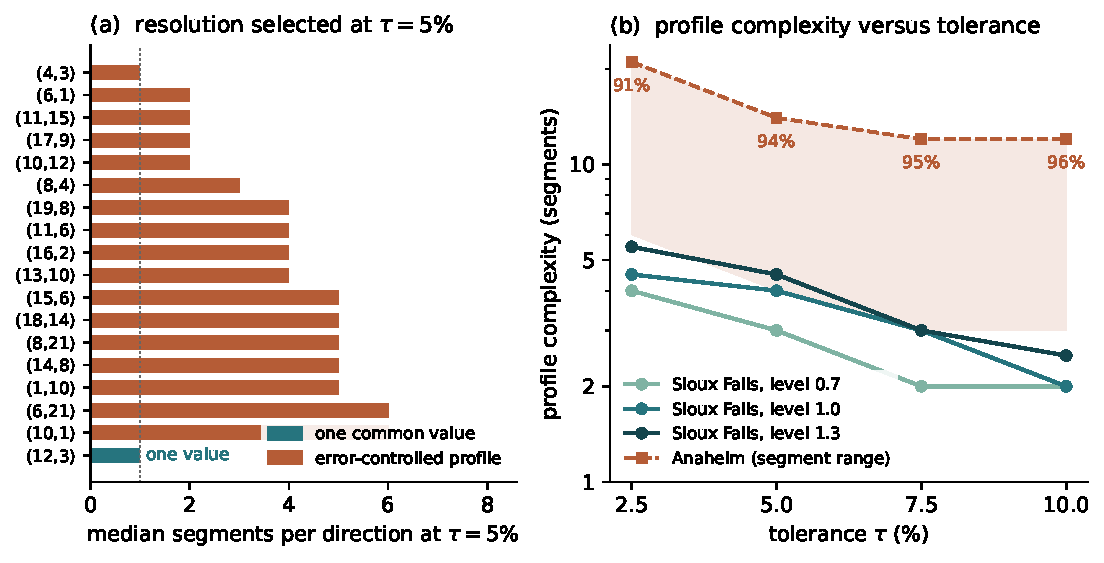
\includegraphics[width=0.99\linewidth]{../figures/fig_v110_summary_frontier.pdf}
\caption{Spatial resolution selected by the error tolerance. Left: the
median minimal segments per projection direction that each of the 18
input-stratified queries receives at the $5\%$ family tolerance
(baseline load; queries sorted by selected resolution; one query is
adequately summarized by a single common value, the remainder by
error-controlled profiles). Right: the profile complexity as the
tolerance varies from $2.5\%$ to $10\%$ --- median segments per
projection direction on Sioux Falls (36 normals, distinct chains
deduplicated, three load levels) and per-query segments on Anaheim's
ordered families; underlying numbers in Table~\ref{tab:tolerance}
(Appendix~\ref{sec:coverage}).}\label{fig:commonsummary}\end{figure}

Figure~\ref{fig:commonsummary} presents the selection and its cost. A
minority of queries admits one common value at a working tolerance;
every other query is summarized one direction at a time. Three counts
should be distinguished when reading these results: the number of
distinct boundary regions $N_{\mathrm{unique}}$, the number of ordered
direction chains $N_{\mathrm{chain}}$ along which they are reported,
and the total number of reported segments $L_{\mathrm{total}}$. On
Sioux Falls the 36 projection normals of the geometric family induce
22--35 distinct ordered chains per query over 1--21 regions each, and
consecutive entries of one chain are nested along that
direction, so the chain --- not the merged sequence --- is the unit of
spatial contiguity; segmenting each chain at the family tolerance
needs a median of $2$--$5.5$ segments per direction across the three
load levels as the tolerance ranges over $2.5$--$10\%$ (at the $5\%$
tolerance and baseline load: median $4$, maximum $8$), with
$L_{\mathrm{total}}$ at a median of $117$ over the distinct chains of
the learned-assignment queries. Per-chain minimality therefore does
not by itself make the reported representation smaller than the
deduplicated set of boundary values; the direction-resolved profiles
are the reported representation there, and the multi-direction counts
quantify direction-specific spatial resolution. Ordering all
directions into one progress sequence yields fewer apparent segments
only by grouping non-adjacent cross-sections, so those counts are not
spatial summaries and are retained only for comparison
(Table~\ref{tab:tolerance}). On Anaheim's single-direction ordered
families --- where the strong compression claims rest --- the same
relaxation raises the compression of the 83--211 attributions
per query from $91.4\%$ (6--21 segments) to $96.4\%$ (3--12
segments). With the same segment count, equal-count partitions have
median worst-segment error $1.4$--$4.0$ times the greedy error per
direction on Sioux Falls and $4.7$--$18.8$ times the tolerance on
Anaheim, so position-aware segmentation is what provides the error
control, not the segment count alone.

The $\pm10\%$ and $\pm20\%$ summaries of the same 18 queries are close in normalized terms, so further subdividing the perturbation width adds little information. The congestion state of the baseline is the more informative axis. All 528 demands are scaled jointly to $0.7$, $1.0$ and $1.3$ times their published values; at each level the level equilibrium is solved once, the focal query alone moves by $\pm20\%$, other demands stay fixed with responsive routes, and the endpoint identity supplies the attribution column (solver protocol in Appendix~\ref{supp:newod}).
\begin{table}[t]\centering\footnotesize
\caption{Common-summary statistics across baseline load levels (18
queries, focal $\pm20\%$, same 36-direction family). Normalized error
is Eq.~\eqref{eq:normerror}; the ratio column is the median
geometric-to-unrestricted spread ratio.}\label{tab:loadlevels}
\begin{tabular}{rrrrrr}\toprule
Level & Queries within $5\%$ & Mixed signs & Median error (\%) & Median ratio & Max.\ negative share\\\midrule
$0.7$ & 2 & 0 & 34.5 & 0.529 & $0.00\%$\\
$1.0$ & 1 & 1 & 44.4 & 0.574 & $0.67\%$\\
$1.3$ & 0 & 3 & 45.2 & 0.563 & $4.03\%$\\
\bottomrule\end{tabular}\end{table}
Table~\ref{tab:loadlevels} shows a monotone pattern: under the light
baseline, attributions are flatter across the family --- the median
normalized error falls to $34.5\%$, two queries satisfy the $5\%$
tolerance and no family crosses zero --- whereas the heavy baseline
makes every query exceed the tolerance, three families mix signs and
the negative share of $(6,21)$ reaches $4\%$. Per-query normalized
errors rise from the light to the heavy level for 17 of 18 queries
(e.g.\ $(10,12)$: $18.6\to35.2\to40.3$; $(1,10)$: $31.2\to44.8\to48.0$).
Across the load levels, light-load conditions admit transferable single
summaries more often, and heavy-load conditions require
boundary-specific reporting. The load-level trend has a theory-side
counterpart: the node-imbalance norm $\norm{d_j}_2$ rises by a factor
of $13.2$ from the light to the heavy baseline, and Eq.~\eqref{eq:cutspread}
sums that imbalance into the spatial range
(Appendix~\ref{sec:coverage} reports the rank correlations and the
Cauchy--Schwarz comparison).

\paragraph{How much does the model-specific level buy?}\label{sec:levelsdiag}
On the synthetic network of Figure~\ref{fig:blockcut}, restricting
attention to the model's path-feasible response envelope restores
boundary consistency despite off-path weight heterogeneity, so the
model-specific level certifies a common boundary value that the universal
condition denies. On Sioux Falls and Anaheim the path-feasible
response envelopes are sufficiently rich that the structural and
model-specific tests both reject a single universal boundary value,
and the diagnosis is stable across load levels
(Appendix~\ref{supp:levelsdiag} reports the numerical diagnosis of the
transferability hierarchy). The realized error-controlled profiles
therefore become the operative representation, and the summaries of
Table~\ref{tab:newod} carry the reporting.


\FloatBarrier
\section{Response-supervised learning for accurate spatial explanations}\label{sec:pairresults}
\paragraph{Hypothesis.}
The boundary-error representation of
Section~\ref{sec:boundarylearning} locates explanation error in the
weighted demand-response discrepancy between the learned and reference
maps. In the studied TSTT setting the weight-shift component of that
discrepancy is small relative to the response component, leading to the
testable hypothesis that supervising the flow Jacobian improves
spatial explanations even when ordinary flow accuracy is already high.
The experiments below compare flow supervision, response supervision
and its weighted form under equal budgets and a common validation-only
weight selection, examine stability when the training budget is
tripled, and measure how many response labels the improvement requires;
the full six-objective family, including the endpoint objectives, is
reported in Appendix~\ref{app:legacy-learning}.

\paragraph{Method and setup.}
The learned map uses the conservative path-share parameterization
\begin{equation}
h_k(q)=q_k\,\operatorname{softmax}\bigl(z_\theta(q)\bigr|_{\Pi_k}\bigr),
\qquad f_\theta(q)=\Delta h(q),
\label{eq:consparam}
\end{equation}
where $\Pi_k$ are the fixed path sets of the assignment structure and
$\Delta$ the path--link incidence: node balance holds identically, and
only the shares are learned. The input is the six-dimensional study
demand vector with background demands fixed at their published levels;
the output covers every path of the structure, so background route
choice responds endogenously. The reference model supplies equilibrium
flows and sensitivity derivatives. Flow supervision fits predicted
flows; response supervision adds the derivative objective
\begin{equation}
\mathcal L(\theta)=\mathcal L_{\mathrm{flow}}
+\lambda_J\,\E_{q,j}\frac{\norm{J_j^L(q)-J_j^S(q)}_2^2}{u_j^2},
\label{eq:learningobjective}
\end{equation}
with $J_j$ the flow Jacobian column of query $j$ and $u_j$ its RMS
training scale; optimizer, batches, validation selection and label
costs appear in Appendix~\ref{app:pairs-v102}. Derivative supervision
itself is established (Sobolev training;
\citealp{czarnecki2017sobolev,yuan2022sobolev}); the target here is
network-derived, and the question is what it contributes to spatial
explanations.
Why the unweighted objective of Eq.~\eqref{eq:learningobjective} acts
on the weighted quantity of Eq.~\eqref{eq:localboundarybound} is
answered by decomposing the weighted response discrepancy at a common
demand state:
\begin{equation}
h_j(q)=\underbrace{\bigl(D^L-D^S\bigr)J_j^S}_{\text{weight shift}}
+\underbrace{D^L\bigl(J_j^L-J_j^S\bigr)}_{\text{response error}},
\qquad h_j=D^LJ_j^L-D^SJ_j^S,
\label{eq:coldecompmain}
\end{equation}
and integrating along the demand path yields the column error
$e_j=\Delta q_j\int_0^1h_j(\gamma(\lambda))\,\mathrm{d}\lambda$. On the
96 test paths the response term dominates overwhelmingly: the
path--query median response and weight norms are $206.5$ and $3.5$
under flow supervision and $147.6$ and $3.3$ under response
supervision, with the response term larger on every path--query pair
for both objectives (Eq.~\eqref{eq:coldecomp} in
Appendix~\ref{app:legacy-learning} states the integrated form).
Supervising the dominant term is therefore a
practical proxy whose effect the boundary metrics measure directly.
\paragraph{Evaluation protocol.}
All objectives are evaluated on the same 96 test demand paths
(Appendix~\ref{app:pairs-v102} states the composition); paths are
the independent unit, metrics average active queries and seeds within
each path, and seed variability is reported separately. Checkpoint and
loss-weight selection use validation data only; the test paths enter
the final report alone.
\paragraph{Primary comparison.}
Table~\ref{tab:pathtable} reports flow prediction, attribution accuracy,
and the end-to-end error of the reported summary on the same test demand
paths for both networks. On the 96 Sioux Falls paths, response
supervision lowers the median attribution-column error from $21.18\%$ to
$14.19\%$ (a relative reduction of one third) and the family-boundary
error from $8.74\%$ to $5.75\%$, while both models retain total-flow
errors near $0.03\%$ (medians $0.0322\%$ and $0.0292\%$). Measured
against the demand-change increment rather than total flows, the
endpoint flow-prediction error falls from $5.03\%$ to $3.52\%$ --- the
incremental response that the attributions decompose --- so response
supervision improves both the attribution column and the response field
it integrates; the total-flow columns stay near $0.03\%$ because total
flows are dominated by the unchanged background. The improvement holds
in every active-query group
(Appendix~\ref{supp:learningdetail}). Path-level paired differences
quantify the uncertainty: the median paired column-error difference is
$-5.03$ percentage points with a path-level bootstrap $95\%$ interval of
$[-6.01,-4.48]$ (10,000 resamples), improving 92 of 96 paths; the
paired family-boundary difference has median $-2.06$ with interval
$[-2.76,-1.65]$, improving 90 of 96, with every group's interval
excluding zero and leave-one-path-out medians varying within
$[-5.11,-4.94]$ and $[-2.11,-2.00]$. The system-contribution difference
is secondary and opposite in sign (median $+0.45$, interval
$[0.01,0.74]$; both methods below $3.5\%$), confirming that scalar
completeness and spatial explanation accuracy measure different
properties. The improvement is consistent across all five seeds, with
both median error metrics decreasing for every seed and 80--91 of 96
paths improving per seed (Table~\ref{tab:fiveseed},
Appendix~\ref{supp:learningdetail}). The same-path decomposition of
Eq.~\eqref{eq:coldecompmain} attributes the discrepancy to demand-response
error on every path--query pair (path--query median response and weight
norms $206.5$ and $3.5$ under flow supervision, $147.6$ and $3.3$ under
response supervision).
\begin{table}[t]\centering\footnotesize
\caption{Prediction and spatial-explanation accuracy, and the end-to-end
error of the reported summary, on the same test demand paths (Sioux
Falls: 96 paths, 24 per active-query group; Anaheim: 48 paths). Entries
are medians of path-level values (active queries and seeds averaged
within each path; flow errors additionally averaged over the path's
states). Total flow: relative flow error; incremental: endpoint
flow-change error (percent of the reference increment norm); column:
attribution-column error; family boundary: maximum boundary error over
the query's family as a percentage of the reference family maximum (the
Sioux Falls family is the geometric screenline set; Anaheim uses its
ordered distance family); final summary: total error of the reported
minimum-segment summary (percent of the reference family scale;
tolerance $5\%$ of the learned family maximum); Seg./chain: median
segments per ordered direction chain (Anaheim's family is one ordered
chain); total segments: median over all distinct chains (Sioux Falls,
18--35 chains per query) or over the single family (Anaheim) --- the two
networks' totals are not comparable one to one.}\label{tab:pathtable}
\setlength{\tabcolsep}{3.4pt}
\begin{tabular*}{\tblwidth}{@{\extracolsep{\fill}}llccccccc}
\toprule
Network & Method & Total flow (\%) & Incremental (\%) & Column (\%) & Family (\%) & Final summary (\%) & Seg./chain & Total seg.\\
\midrule
Sioux Falls & Flow & 0.032 & 5.03 & 21.18 & 8.74 & 11.35 & 3.6 & 117\\
Sioux Falls & Response & 0.029 & 3.52 & 14.19 & 5.75 & 8.68 & 3.6 & 117\\
\addlinespace
Anaheim & Flow & 0.024 & 2.46 & 1.64 & 0.94 & 4.57 & 9.9 & 9.9\\
Anaheim & Response & 0.019 & 2.03 & 1.31 & 0.78 & 4.55 & 9.9 & 9.9\\
\bottomrule\end{tabular*}\end{table}

\paragraph{Where the flow-only explanation breaks, and what supervision
repairs.}
Figure~\ref{fig:repair} shows one pre-specified case: among the 96 test
paths, the one whose paired family-error improvement is closest to the
median improvement (path 22, six active queries; improvement $48.4$
against the median $49.2$), and within it the query with the largest
flow-only family error, OD $(7,12)$. The panels display the query's
longest projection-direction chain (20 nested boundaries, a geometric
display choice independent of attribution values), the boundary error
against the reference along that chain, and the family-wide worst
boundary on the network. The flow-only model does not merely rescale
the profile: it misplaces the attribution across the corridor, with
errors concentrated where the reference profile varies. At the worst
flow-only boundary ($369.5$ TSTT units, on a reference value of
$5{,}619.3$ that is congestion-dominated: $5{,}018.7$ of it from
congestion weights against $600.6$ from free-flow weights) the error
falls to $80.1$ under response supervision --- a $78\%$ reduction at
that boundary; over the whole family, the worst error falls from
$369.5$ to $115.2$ and the end-to-end error of the reported summary
from $679.1$ to $463.7$ at essentially unchanged segment count ($186$
to $190$ over the family). All quantities come from the same
five-seed-median columns the figure displays. The segment summaries of
all three columns sit inside their stated tolerance bands, so the
repair acts on the profile the summaries compress, not on the
compression itself.
\begin{figure}[t]
\centering
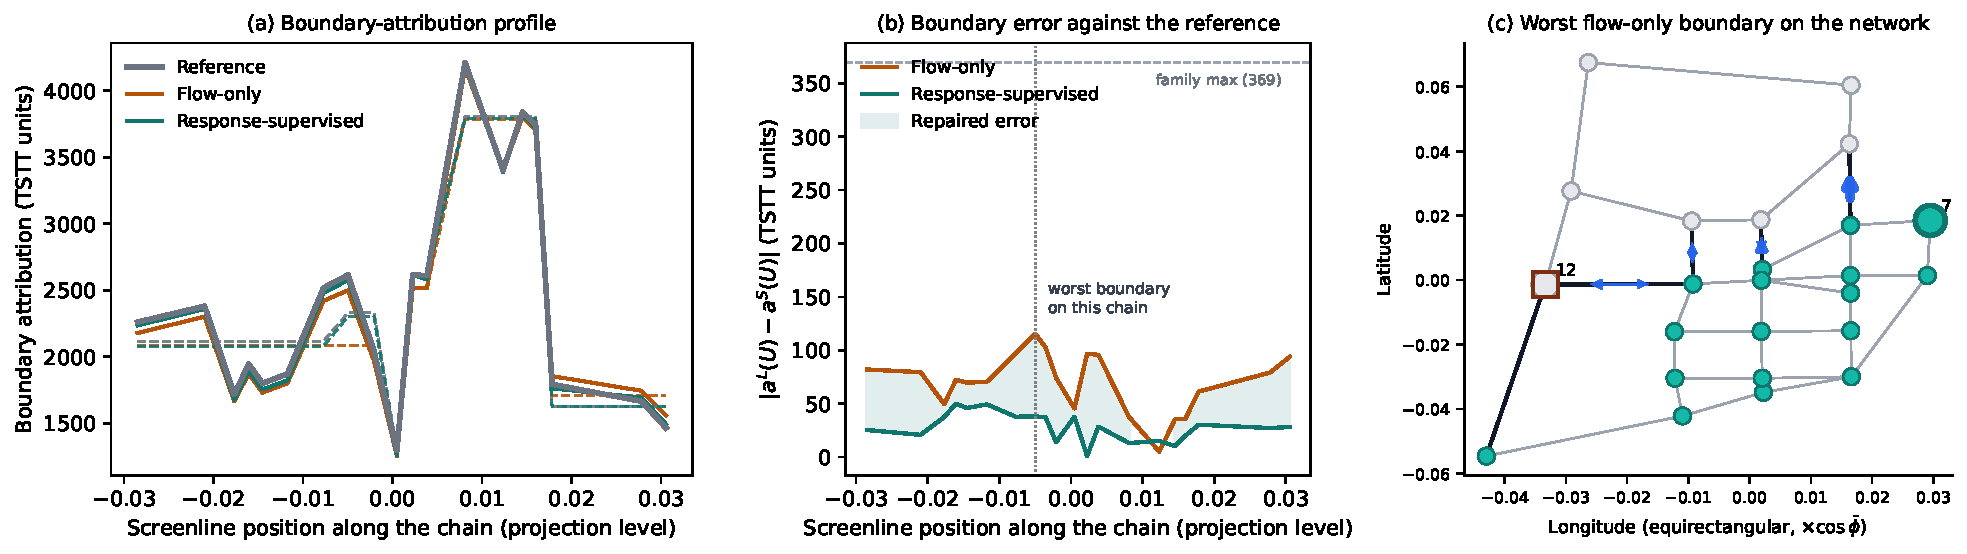
\includegraphics[width=\linewidth]{../figures/fig_v111_repair.pdf}
\caption{A learned spatial profile repaired by response supervision
(pre-specified case: path 22, query $(7,12)$; five-seed median columns).
(a)~Boundary-attribution profile along the query's longest
projection-direction chain (20 nested boundaries at the $10^\circ$
direction): reference (gray), flow-only (ochre), response-supervised
(teal), each with its minimum-segment summary (dashed). (b)~Boundary
error against the reference along the same chain; the dotted line marks
the worst boundary on the chain and the gray dashed line the
family-wide maximum ($369.5$). (c)~The family-wide worst flow-only
boundary on the network: teal nodes form $U$ (origin $7$ ringed,
destination $12$ square); arrow width scales with the signed
crossing-link contribution (solid blue positive, dashed red
negative).}\label{fig:repair}
\end{figure}

\paragraph{The objective family.}
The boundary-error representation of
Eq.~\eqref{eq:localboundarybound} defines a family of supervision
objectives rather than a single loss; the complete six-objective
comparison, including the weighted form identified by
Eq.~\eqref{eq:coldecompmain} and the boundary-seminorm loss, appears
in Appendix~\ref{app:legacy-learning}. Two of its results organize the
present comparison. The unweighted response objective attains the
lowest errors on every metric (column $14.19\%$, family boundary
$5.75\%$, flow $0.029\%$) with the widest usable weight range, while
its weighted form reaches $15.21\%$ --- the weight-shift term the
unweighted objective ignores is small. And $\mathcal K_j$ is a seminorm
whose kernel contains the circulation directions, so optimizing the
boundary value alone cannot restore the response field the profile
integrates: the boundary-seminorm objective attains the lowest
validation boundary error yet a test column error above flow-only
training ($24.18\%$, improving only 8 of 96 paths).

\paragraph{Label efficiency, training budget, and wall-clock.}
The improvement is cheap in labels and stable in budget. Retraining at
per-query derivative-center budgets of 6--48 (36--288 centers; full
budget 384) reaches half of the full column-error improvement at 36
centers and $90\%$ at 288, with subset interquartile ranges below
$0.8$ percentage points and flow accuracy unchanged
(Figure~\ref{fig:v109labelbudget}, Appendix~\ref{app:labelbudget}).
Tripling the continuation budget to 3{,}600 updates improves both
methods on both networks while the response curve stays below the flow
curve at every update count (Figure~\ref{fig:v109convergence},
Appendix~\ref{supp:learningdetail}): the median column error falls to
$19.46\%$ against $11.41\%$ on Sioux Falls and $1.24\%$ against
$0.88\%$ on Anaheim. Derivative supervision costs more per update
($1.8\times$ on Sioux Falls, $3.3\times$ on Anaheim); on Sioux Falls
the anytime dominance survives the cost difference in wall-clock
terms, while on Anaheim the response run reaches the flow method's
final error after about $2.2$ times its training time.

\paragraph{End-to-end explanation error.}
The quantities of Table~\ref{tab:pathtable} concern the learned
profiles; the reported artifact is the learned model's minimum-segment
summary, whose total error Table~\ref{tab:pathtable} already carries as
the budget of Eq.~\eqref{eq:totalbudget} at the working $5\%$ tolerance.
Figure~\ref{fig:v110resolution} traces the same quantities as the
tolerance --- and with it the number of reported segments --- varies
from $0.5\%$ to $10\%$, and Table~\ref{tab:matched} reports the
matched-complexity comparison over that pre-specified grid: at each
tolerance the two methods segment their own learned profiles, and the
paired difference is evaluated at the matched segment budget --- the
smaller of the two methods' per-path segment counts, each method
interpolated on its own error--segments grid.
The two networks occupy different regimes, and the error budget
identifies the effective lever on each. On Sioux Falls the model term
dominates ($8.74\%$ against a $4.76\%$ summary term under flow
supervision), the response-supervised curve lies below the
flow-supervised curve at every segment count: at the matched segment
budget of each tolerance (Table~\ref{tab:matched}) the paired median
difference is $-1.7$ to $-2.0$ percentage points with bootstrap
intervals excluding zero at every tolerance --- computed on all 96
paths' data at $0.5$--$2.5\%$ and on the common-support subset at the
two loosest tolerances, where the equal-tolerance comparison over all
paths is essentially identical (individual paths can still move the
other way; the intervals are for the median) --- and the iso-error view
quantifies the
saving: a final error of $11.0\%$ needs $152$ segments under flow
supervision but $117$ under response supervision, while the $8.8\%$
error that response supervision attains with $117$ segments is not
reached by flow supervision anywhere in the grid (its best, $8.80\%$,
requires $233$ segments). On Anaheim the learned columns are closer to
the reference, and at the working $5\%$ tolerance the budget is
compression-dominated: the summary term ($4.3\%$) is several times the
model term ($0.9\%$), both curves track the reference-compression
curve --- the error of compressing the reference profile itself at each
tolerance --- and the two methods are nearly indistinguishable in the
final error ($4.57$ against $4.55$), exactly as the budget predicts:
the model error is not the active bottleneck there, and tolerance
refinement, not a better learned response, is the effective
intervention. At the tightest $0.5\%$ tolerance the model term takes
over ($0.9\%$ and $0.8\%$ against a $0.5\%$ summary term), where the
response-supervised final error is again lower ($0.91\%$ against
$1.06\%$). Better learned responses matter precisely when model error
is the active bottleneck; when compression dominates, the framework
correctly identifies tolerance refinement as the relevant lever. On
both networks the measured total error of the reported summary stays
within the budget on every path. Relative to the baselines,
segmentation cuts the total error by a factor of $3.0$--$3.8$ (single
common value) and $1.7$--$2.0$ (equal-count) on Sioux Falls, and by
$10.5$--$10.6$ and $10.2$ on Anaheim --- where the strongly ordered
profiles make equal-count segmentation nearly as coarse as a single
value, so position-aware segmentation is what carries the error
control. The final-summary entries of Table~\ref{tab:pathtable} are
medians of budget components computed on each path--query--seed before
aggregation, so they do not add to a guarantee for any single
explanation.

\begin{table}[t]\centering\footnotesize
\caption{Matched-complexity end-to-end comparison over the
pre-specified tolerance grid. At each tolerance both methods segment
their own learned profiles. $L$: median total segment count (Sioux
Falls: distinct chains; Anaheim: single ordered family). Error: median
normalized total error of the reported summary (percent of the
reference family scale, as in Table~\ref{tab:pathtable}). The paired
difference is computed at the matched segment budget
$L^{*}=\min(L_{\mathrm{flow}},L_{\mathrm{response}})$ of each path:
each method is interpolated linearly on its own five-point
(error,~segments) grid, and the median per-path paired difference
(response $-$ flow) receives a path-level bootstrap $95\%$ interval
(5{,}000 resamples). Only paths whose $L^{*}$ lies inside both
methods' grid support are compared ($n$; budgets outside a grid are
excluded, not clamped): all 96 Sioux Falls paths at $0.5$--$2.5\%$,
95 at $5\%$, and 14 at $10\%$, where the two grids barely overlap;
all 48 Anaheim paths except 13 at $10\%$. The equal-tolerance medians
(no interpolation, all paths) differ from the tabulated differences by
at most $0.11$ percentage points and exclude zero at every tolerance
on both networks.}\label{tab:matched}
\setlength{\tabcolsep}{4.2pt}
\begin{tabular*}{\tblwidth}{@{\extracolsep{\fill}}lrrrrrrr}
\toprule
 & \multicolumn{2}{c}{Flow} & \multicolumn{2}{c}{Response} & \multicolumn{3}{c}{Matched-budget difference}\\
\cmidrule(lr){2-3}\cmidrule(lr){4-5}\cmidrule(l){6-8}
Tolerance & $L$ & Error (\%) & $L$ & Error (\%) & $L^{*}$ & $n$ & Median (pp) [$95\%$ interval]\\
\midrule
\multicolumn{8}{l}{\emph{Sioux Falls} (96 paths; model-error dominated)}\\
$0.5\%$ & 233 & 8.80 & 235 & 5.82 & 233 & 96 & $-2.02$ $[-2.70,-1.60]$\\
$1\%$ & 202 & 9.01 & 201 & 6.04 & 201 & 96 & $-1.98$ $[-2.68,-1.64]$\\
$2.5\%$ & 152 & 9.63 & 152 & 6.91 & 152 & 96 & $-1.93$ $[-2.59,-1.49]$\\
$5\%$ & 117 & 11.35 & 117 & 8.68 & 117 & 95 & $-1.68$ $[-2.41,-1.28]$\\
$10\%$ & 77 & 13.93 & 77 & 11.51 & 25 & 14 & $-1.78$ $[-3.06,-1.25]$\\
\addlinespace
\multicolumn{8}{l}{\emph{Anaheim} (48 paths; compression dominated at $5\%$)}\\
$0.5\%$ & 28 & 1.06 & 27 & 0.91 & 27 & 48 & $-0.16$ $[-0.20,-0.08]$\\
$1\%$ & 21 & 1.37 & 21 & 1.24 & 21 & 48 & $-0.11$ $[-0.17,-0.07]$\\
$2.5\%$ & 12 & 2.54 & 12 & 2.49 & 12 & 48 & $-0.06$ $[-0.08,-0.02]$\\
$5\%$ & 10 & 4.57 & 10 & 4.55 & 10 & 48 & $-0.02$ $[-0.04,-0.01]$\\
$10\%$ & 6 & 8.14 & 6 & 8.13 & 6 & 35 & $-0.03$ $[-0.05,-0.01]$\\
\bottomrule\end{tabular*}\end{table}

\paragraph{Beyond the labeled response domain.}
Both the derivative centers and the 96 test paths draw base demands
from $[0.65,1.3]$ times the published OD vector, so the improvement
could be specific to that labeled band. Two out-of-domain bands ---
low loads on $[0.40,0.60]$ and high loads on $[1.35,1.55]$, 24 paths
each under the test generator's rules --- separate the two
extrapolation directions. On the high-load band, adjacent to the
labeled domain, response supervision remains better on every metric
(paired medians: column $-1.31$, family boundary $-0.68$, unrestricted
extrema $-5.30$ percentage points, all intervals excluding zero). On
the low-load band, far from the labeled domain, the advantage
disappears: the family-boundary and summary errors are slightly higher
under response supervision (paired medians $+0.68$ and $+0.57$
percentage points, intervals $[+0.18,+1.06]$ and $[+0.07,+0.90]$),
with the column error statistically indistinguishable ($+1.25$,
$[-0.17,+2.99]$). Response supervision therefore provides its gain
inside and near the labeled response domain and preserves the error
ordering under moderate extrapolation toward higher loads; the low-load
band marks where the labeled derivative information stops
transferring (Appendix~\ref{app:pairs-v102}).
\begin{figure}[t]
\centering
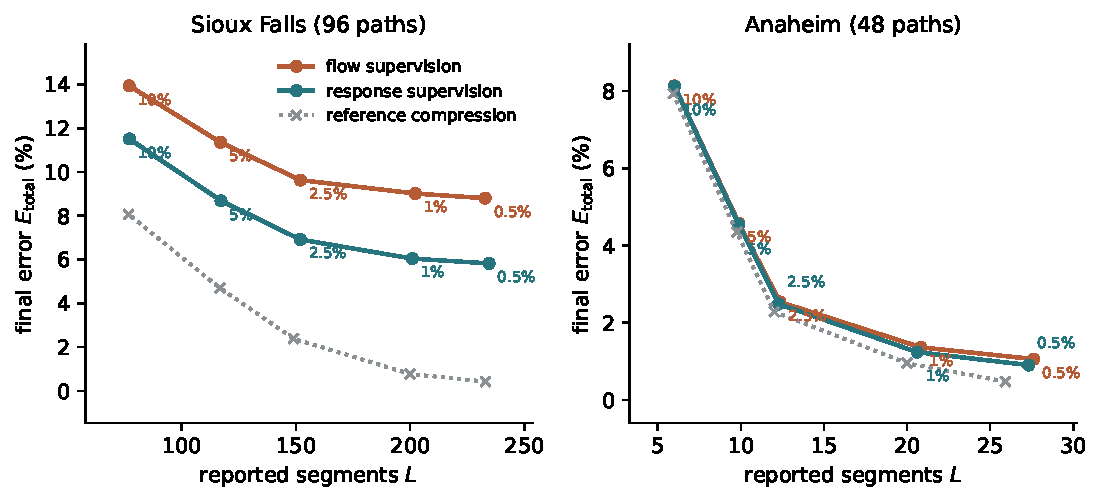
\includegraphics[width=\linewidth]{../figures/fig_v110_resolution.pdf}
\caption{Final error of the reported summary against the number of
reported segments, as the family tolerance varies over $0.5$--$10\%$
(annotated; percent of the learned family maximum). Sioux Falls
(left): model-error dominated --- the response-supervised curve (teal)
lies below the flow-supervised curve (ochre) at every segment count, so
better responses convert into either fewer segments at equal accuracy
or more accurate summaries at equal complexity. Anaheim (right):
compression dominated at the working tolerance --- both curves track
the gray reference-compression curve, the error of compressing the
reference profile itself at each tolerance, plotted at its own segment
count ($\times$ marks). Per-tolerance segmentation recomputed from the
final learned profiles; common per-query normalization as in
Table~\ref{tab:pathtable}.}\label{fig:v110resolution}
\end{figure}

\paragraph{Bound tightness.}
Computed with the same $41$-state trapezoidal quadrature for both
sides, the exact unrestricted errors $\mathcal K_j(e_j)$ lie below the
integrated bounds $B_j$ of Eq.~\eqref{eq:localboundarybound} (the
numerical verification and quadrature accuracy are reported in
Appendix~\ref{supp:accuracy}). The chain is tight: the median ratio
$\mathcal K_j(e_j)/B_j$ is $0.95$ for flow supervision (quartiles
$0.91$--$0.98$) and $0.95$ for response supervision (quartiles
$0.90$--$0.97$). The integrated bound is therefore a tight
\emph{a posteriori} upper bound on the realized worst boundary error
--- it uses reference-response information, as
Section~\ref{sec:totalbudget} notes --- and response supervision lowers
the family, unrestricted and bound levels in parallel. The geometric
family retains about half of the unrestricted error (median ratio
$E^{\mathrm{geo}}/\mathcal K_j(e_j)$ $0.51$ and $0.48$), so the
single-family errors reported throughout should be read as lower
bounds on the worst separating-region error.

\paragraph{Second network: Anaheim.}
We repeat the comparison on Anaheim by training independently on the
second network, using the same conservative parameterization,
objective set and evaluation principles, with the network-specific
training and validation settings stated in
Appendix~\ref{app:anaheimlearning} (the six largest published OD
demands are the study queries; all remaining positive demands stay
fixed with endogenous route choice over the same ten-path
centroid-restricted structure as Section~\ref{sec:anaheim}; the model
outputs all $14{,}060$ path flows; forty-eight test demand paths ---
twelve per active-query group, same generation rule, fresh seed ---
are solved at a 21-state quadrature with reference sensitivities);
the Anaheim rows of Table~\ref{tab:pathtable} report the outcome.
Anaheim's attribution columns are easier to learn than Sioux
Falls' --- the free-flow-weighted response dominates the column and
both objectives reach column errors near $1.5\%$ --- but the ordering
is the same and is consistent across seeds: response supervision
lowers the median column error from $1.64\%$ to $1.31\%$ and the
family-boundary error from $0.94\%$ to $0.78\%$, improves $46$--$48$
of $48$ paths in column error and $44$--$47$ of $48$ in
family-boundary error across the five seeds, and does so while flow
accuracy is again indistinguishable ($0.024\%$ and $0.019\%$) and the
incremental flow error falls from $2.46\%$ to $2.03\%$.
Path-level paired bootstrap quantifies the uncertainty of the smaller
Anaheim margins (10,000 resamples, paths as resampling unit, seeds
averaged within path): the median paired column-error difference is
$-0.29$ percentage points with a $95\%$ interval of $[-0.33,-0.21]$,
improving all $48$ paths, and the paired geometric difference is
$-0.17$ with interval $[-0.19,-0.10]$, improving $47$ of $48$; both
intervals exclude zero, and each of the five seeds shows the same
direction with its interval excluding zero. The
reported summaries inherit the same budget structure as Sioux Falls
(absolute path medians: model term $17.0\to13.1$, summary term at the
tolerance, $99.7$ and $99.3$ vehicle-minutes per hour; normalized in
Table~\ref{tab:pathtable}); the total stays within the budget on every
path, and the paired total error improves on $73.3\%$ of path--seed
units. At the selected $5\%$ tolerance Anaheim's total error is
compression-dominated --- the model term is below one percent of the
family scale --- so further reduction of the reported summaries must
come primarily from a tighter tolerance, with model improvement raising
the ceiling once the tolerance tightens (Figure~\ref{fig:v110resolution}
traces both levers). The direction of every conclusion --- better
explanations from response supervision, and a dominant response term
--- therefore does not depend on the network; which term dominates the
total error does: at the working tolerance the Anaheim budget is
compression-dominated while the Sioux Falls budget carries the larger
model term, as the error budget makes explicit.


\FloatBarrier
\section{Conclusions}\label{sec:conclusions}
An OD demand effect should be represented neither by one global scalar
nor by an unstructured link map, but by the coarsest
boundary-attribution profile whose physical and approximation errors
are explicitly controlled. The three parts of the paper deliver that
representation in sequence.

Topology characterizes when one transferable value is guaranteed
uniformly over all flow-conserving responses: for two-sided connected
regions, precisely when the marginal outcome weights agree on the block
atoms traversed by the queried OD paths. Multiple queries merge these
atoms transitively, so the admissible explanation is a query-dependent
structural property rather than a global network attribute, identified
before any model is trained. For a learned assignment map this theorem
is a structural certificate, checkable at every state along the
attribution path.

When one value is insufficient, node divergence determines what is
reported: the exact attribution range, the minimax common summary and
its error, minimum-segment summaries with explicit approximation
errors, and the maximum disagreement between learned and reference
explanations. The adaptive reporting rule allocates spatial resolution
only where the network response requires it, and the reported summary
carries a total error budget that separates model error from
compression error. Structural compatibility and compression are
certified from the learned model and the reported profile alone;
learned-reference fidelity is an offline validation guarantee requiring
reference assignments.

For learned assignment, response supervision --- the training mechanism
the error budget identifies --- improves the reported explanation at
matched cost. At every segment count on the pre-specified tolerance
grid the response-supervised final error is lower on both networks,
with paired intervals excluding zero; on Sioux Falls the error that
flow supervision cannot reach within the grid ($8.8\%$ at 233 segments)
is attained by response supervision with 117 segments, and an $11\%$
error needs $35$ fewer segments. The mechanism ablation shows the gains
are structural rather than an artifact of the pretraining recipe: the
exact path-share parameterization dominates direct conservation
mechanisms under either pretraining loss, and derivative supervision
improves every mechanism. The improvement extends beyond the labeled
response domain on the high-load side; on the low-load side the
advantage disappears, marking the boundary of the labeled regime.
Accurate flow prediction is not sufficient for spatially trustworthy
OD explanations; together, these results turn spatial attribution from
an ad hoc boundary aggregation into a transport-specific,
mathematically controlled and learnable explanation framework.

\paragraph{Limitations.}
The analysis fixes the road representation, outcome definition,
attribution path, and admissible boundary family; subdividing roads
changes which crossing-link costs a boundary includes. Per-query
attributions under joint demand changes are path-specific, although
their signs, summary-error levels, and mechanism rankings were stable
across the twenty-two tested alternative orders
(Section~\ref{subsec:pathrobust}). The numerical evidence concerns
static fixed-path logit-SUE models on two benchmark networks; extending
the framework to dynamic assignment and broader demand domains remains
a direction for future work.

\section*{Code and data availability}
Code, configurations, processed result arrays, and scripts reproducing
all tables and figures are available through an anonymized archival
repository; its access link accompanies the submission. The archive
records software versions, random seeds,
TNTP checksums, and the generating script for each reported result;
trained checkpoints are regenerated by the released scripts under the
fixed seeds. Public access will be enabled upon acceptance.
The Sioux Falls and Anaheim networks and demands are available from the public
\href{https://github.com/bstabler/TransportationNetworks/tree/master/SiouxFalls}{Sioux Falls TNTP repository}
and \href{https://github.com/bstabler/TransportationNetworks/tree/master/Anaheim}{Anaheim TNTP repository}
\citep{tnfrc2024transportation}; training targets are synthetic fixed-path
logit-SUE assignments.
\section*{Declaration of competing interest}
The authors declare that they have no known competing financial interests
or personal relationships that could have appeared to influence the work
reported in this paper.
\FloatBarrier
\bibliographystyle{cas-model2-names}
\setlength{\bibsep}{0.8pt plus 0.2pt}
\bibliography{references_v112}
\appendix
\counterwithin{theorem}{section}
\counterwithin{rmk}{section}
\counterwithin{table}{section}
\counterwithin{figure}{section}
\counterwithin{equation}{section}
%% Mathematical appendix for the focused v82 revision.
\section{Mathematical foundations and proofs}\label{app:proofs}

\subsection{Conventions and conservation transfer}\label{app:notation}
The incidence matrix $B\in\R^{n\times m}$ has entries $-1$ at an arc's
origin and $+1$ at its destination; $\mu_j=e_{t_j}-e_{s_j}$ and
$M=[\mu_1,\ldots,\mu_K]$. Write $Z=\ker B$ and let $B^\dagger$ be the
Moore--Penrose pseudoinverse. All norms below are Euclidean or their
induced operator norms unless indicated otherwise. Graphs are loopless
multigraphs: parallel and reciprocal arcs remain distinct edges, including
in two-edge cycles. Block atoms and the block-cut tree are taken on the
underlying undirected multigraph. Formally, $\iota(v)$ is the cut-vertex
node when $v$ is an articulation vertex and otherwise its unique block
node; $\mathcal P(s,t)$ lists the atoms on the unique tree path from
$\iota(s)$ to $\iota(t)$. A signed simple $s$--$t$ path vector $p$ satisfies
$Bp=\mu$ and the full solution set is $p+Z$. Such a path uses only atoms
of $\mathcal P(s,t)$ and meets every atom on it.

\paragraph{Signed responses.}\label{app:signed}
The circulation and response vectors are signed first-order sensitivities,
not nonnegative commodity flows. At a strictly positive flow, sufficiently
small signed circulation perturbations also preserve nonnegativity. A
restricted response family is treated explicitly below.

\begin{corollary}[IG exchange]\label{cor:ig}
For an exactly conservative $C^1$ field on an open neighborhood of the
attribution path, $Bg_j=\mu_j\Delta q_j$ (Eq.~\eqref{eq:anchorchain}).
\end{corollary}
\begin{pf}
Differentiate $Bf(q)=Mq$ to obtain $BJ_f(q)=M$, then integrate the
$j$th column along $\gamma(\lambda)=q^0+\lambda\Delta q$.
\end{pf}

\subsection{Cycle structure and the classification proofs}\label{app:classificationproof}
\begin{lemma}[structure of circuit classes]\label{lem:mprime}
The non-bridge atoms are the non-singleton circuit classes; each bridge
is a singleton class. Moreover $Z=\bigoplus_A Z_A$, where
$Z_A=\{z\in Z:\operatorname{supp}z\subseteq A\}$, and the summands
have disjoint edge supports.
\end{lemma}
\begin{pf}
No simple cycle crosses an articulation vertex into another block: it
would revisit that vertex. Within a non-bridge block, any two edges lie
on a common cycle. One way to see this is to subdivide the two edges;
the resulting block is still biconnected, so its two new vertices lie
on a common cycle, which descends to the required cycle. This is the
usual circuit-class characterization of the graphic matroid
\citep{oxley2011matroid}. Every signed circulation is a linear combination
of signed simple-cycle vectors: subtract the fundamental cycles of a
spanning forest to leave a circulation on a forest, necessarily zero
by successive leaf elimination. Grouping these cycles by their blocks
gives the direct sum, and distinct blocks have disjoint edge sets.
\end{pf}

\begin{lemma}[circulation-preserving diagonal maps]\label{lem:m}
For $D=\operatorname{diag}(w)$, $DZ\subseteq Z$ if and only if $w$ is
constant on every non-bridge atom; bridge weights are free.
\end{lemma}
\begin{pf}
For any signed simple-cycle vector $z_C$, a circulation supported on
that cycle has equal signed amplitudes on successive edges, by node
balance. Thus $BDz_C=0$ forces $w$ constant on $C$, and
Lemma~\ref{lem:mprime} propagates equality throughout each atom.
Conversely, atomwise constancy makes $D$ a scalar on every $Z_A$, so
it preserves their direct sum. Bridges carry no circulation.
\end{pf}

\begin{pf}[Theorem~\ref{thm:t3cpmain}]
Add a virtual reverse OD edge $(t,s)$ and set
\[
\bar B=[B,-\mu],\qquad \bar D=\operatorname{diag}(w,\alpha).
\]
For a fixed $\alpha$, property~\eqref{eq:t3prop} is equivalent to
$\bar D\ker\bar B\subseteq\ker\bar B$.
Indeed, a kernel vector $(x,a)$ obeys $Bx=a\mu$. If $a\ne0$,
apply \eqref{eq:t3prop} to $x/a$ to obtain $BDx=a\alpha\mu$.
If $a=0$, subtract the identities for $p+x$ and $p$, with any fixed
$Bp=\mu$, to obtain $BDx=0$. These are exactly the two cases of
$\bar B\bar D(x,a)=0$. Conversely, applying kernel invariance to
$(x,1)$ gives \eqref{eq:t3prop} for every $Bx=\mu$, at that same $\alpha$.

By Lemma~\ref{lem:m}, this invariance holds precisely when the augmented
weights are constant on its block atoms. The virtual edge and a simple
$s$--$t$ path form a cycle meeting every original atom on
$\mathcal P(s,t)$, so these atoms merge with the virtual edge into one
circuit class. No other atoms join it: every new simple cycle contains
the virtual edge and a simple $s$--$t$ path, which uses only those
atoms. Other original atoms retain their classes. Thus the augmented
criterion is exactly within-atom constancy everywhere and common value
$\alpha$ on $\bigcup\mathcal P(s,t)$. This proves both directions and
identifies $\alpha=w^*$ without changing the universal response family.
\end{pf}

\begin{pf}[Theorem~\ref{thm:t3cm} and Corollary~\ref{cor:path}]
Apply the single-OD theorem to each query at the same $w$. Necessity
requires equality within every atom and among all atoms co-traversed
by a queried block path. Their transitive closure is exactly the
compatibility-class partition. Conversely, class constancy supplies
both single-OD conditions for every query. Along the attribution
path, exact conservation gives $BJ_f(\gamma(\lambda))\mathbf e_j=\mu_j$;
the static theorem therefore yields
\[
Bc_j=\Delta q_j\int_0^1
BD_\lambda J_f(\gamma(\lambda))\mathbf e_j\,d\lambda
=\Delta q_j\left(\int_0^1w^*_{k(j)}(\lambda)\,d\lambda\right)\mu_j.
\]
\end{pf}

\begin{corollary}[all-OD class collapse]\label{cor:allod}
Requiring the criterion at one common $w$ for every ordered pair of
distinct vertices makes all atoms in a connected component share one
constant.
\end{corollary}
\begin{pf}
For two atoms incident to the same cut vertex, choose endpoints on
their opposite sides. Their OD block path contains both atoms, forcing
their constants to agree. Connectivity of the block-cut tree propagates
the equality throughout the component.
\end{pf}

\begin{rmk}[a common flow realization]\label{rmk:quantifier}
The merging proof requires one common weight vector. Computing the
queries at different realized flows does not in general supply this
premise.
\end{rmk}

\paragraph{Example~B: query-dependent compatibility under the
unrestricted criterion.}
This example uses the uniform pendant configuration of
Figure~\ref{fig:blockcut} --- all three $D$ weights equal to $3$ ---
and evaluates the unrestricted criterion over all $512$ separating sets
per query, complementing the connected-region Example~A of the main
text, whose heterogeneous pendant is invisible to queried connected
boundaries.
\begin{table}[pos=tb]
\footnotesize
\caption{Constructive query-dependent compatibility on Figure~\ref{fig:blockcut}
of the main text, uniform pendant weights. Ranges use all $512$
separating sets per query and a
conservative unit response; the weighted circulation residual is below
$5\times10^{-16}$ in all stages, so these ranges are independent of that
response. The intentionally chosen linear weights illustrate
compatibility; they are not the marginal costs of the original TSTT
outcome.}\label{tab:topologyexample}
\begin{tabular*}{\tblwidth}{@{\extracolsep{\fill}}lccccl}
\toprule Stage & $w_{A,b_1,B}$ & $w_{b_2,C}$ & $w_D$ & Queried ODs & Account ranges\\\midrule
Initial query & 1 & 2 & 3 & $(s,u)$ & $[1,1]$\\
Add query & 1 & 2 & 3 & $(s,u);(u,t)$ & $[1,1];[1,2]$\\
Adjust merged class & 1 & 1 & 3 & $(s,u);(u,t)$ & $[1,1];[1,1]$\\
\bottomrule\end{tabular*}\end{table}
The calculation uses the minimum-norm solution of $Bx=\mu$ and checks
$BDZ=0$ on a basis of $\ker B$, which establishes response independence
of the displayed boundary vector. The theorem supplies the uniform
common-value guarantee in stages one and three.

\subsection{Direction, integration, and network representation}\label{supp:criteria}
At fixed weights $D=\operatorname{diag}(w)$, a realized model balances
when $BDJ_j=\alpha_j\mu_j$ for its actual response.
\emph{Universal directional balance} requires
$BDx\in\operatorname{span}\{\mu_j\}$ for every $Bx=\mu_j$, allowing its
coefficient to depend on $x$; \emph{structural cut consistency}
additionally requires one common coefficient across all such responses,
and is the property classified in the main text. For non-collinear
queries with shared weights, universal directional balance already
implies structural cut consistency because
$BD\ker B\subseteq\bigcap_j\operatorname{span}\{\mu_j\}=\{0\}$;
a query and its reverse alone do not suffice.
\begin{proposition}[universal directional criterion]\label{prop:directional}
Let $\hat x_j=B^\dagger\mu_j$, let $N$ span $Z$ with orthonormal
columns, and let $P_{\mu_j}$ project orthogonally onto
$\operatorname{span}\{\mu_j\}$. At fixed $w$, universal directional
balance is equivalent to
\[
(I-P_{\mu_j})BD\hat x_j=0,\qquad (I-P_{\mu_j})BDN=0.
\]
The scale may depend on the response. Requiring one common boundary value
additionally requires $BDN=0$. If directional balance holds along the
whole path for a conservative model, its integrated column balances.
\end{proposition}
\begin{pf}
Every response is $\hat x_j+z$, $z\in Z$. Apply $I-P_{\mu_j}$ to
$BD(\hat x_j+z)$ and vary $z$. The scale is
$\mu_j^\top BD(\hat x_j+z)/\norm{\mu_j}^2$ and is independent of
$z$ precisely when $BDZ=0$. Integrating the realized directional
identity gives the endpoint conclusion. Equivalently, invariance on
all incidence fibers, $Bx=By\Rightarrow BDx=BDy$, is exactly
$DZ\subseteq Z$, since $x-y$ ranges over $Z$.
\end{pf}

\begin{example}[strict separation of the criteria]\label{ex:triangle}
On the diamond $(s,a),(a,t),(s,b),(b,t)$ with weights $(1,1,1,2)$,
the upper-path response $(1,1,0,0)$ has divergence $\mu$ after
weighting, but the lower-path response has weighted divergence
$(-1,0,-1,2)$ in node order $(s,a,b,t)$, outside $\operatorname{span}\{\mu\}$.
On the triangle $(s,t),(t,u),(u,s)$ with weights $(1,0,0)$, every
response $x=(1+c,c,c)$ satisfies $BDx=(1+c)\mu$; direction balances,
but the common boundary value fails because the circulation $(1,1,1)$ maps
to $\mu\ne0$.
\end{example}

If directional balance holds for all
queries at common $w$, differences give
$BDZ\subseteq\bigcap_j\operatorname{span}\{\mu_j\}$. For non-collinear
queries this intersection is $\{0\}$, so directional balance implies
the common-value property. This uses the full response space $Z$.

\paragraph{Restricted families.}\label{app:membership}
For $S\subseteq Z$ with basis $N_S$, test responses in
$x_j^{\mathrm{ref}}+S$, where $Bx_j^{\mathrm{ref}}=\mu_j$.
The same proof gives the direction tests with $\hat x_j,N$ replaced
by $x_j^{\mathrm{ref}},N_S$; common boundary value replaces the second test by
$BDN_S=0$. Using $\hat x_j$ requires
$\hat x_j-x_j^{\mathrm{ref}}\in S$. For a fixed-path model $f=\Delta h$,
$A_{\mathrm{OD}}h(q)=q$ and $B\Delta=MA_{\mathrm{OD}}$. Choose a path
vector $a_j$ with $A_{\mathrm{OD}}a_j=\mathbf e_j$ and set
$x_j^{\mathrm{ref}}=\Delta a_j$. Differentiation yields
\[
J_f\mathbf e_j-x_j^{\mathrm{ref}}
=\Delta(\partial_jh-a_j)\in\Delta\ker A_{\mathrm{OD}}=:T_{\mathrm{swap}}.
\]
This space includes OD path exchanges of every OD: background
ODs may reroute even when their demands remain fixed.

\begin{example}[endpoint cancellation]\label{ex:cancellation}
For two series bridges, $f(q)=(q,q)$ and
$T(F)=F_1+F_2+[\sin(2\pi F_1)-\sin(2\pi F_2)]/(2\pi)$ give
\[
c_1-c_2
=\frac{\sin(2\pi q^1)-\sin(2\pi q^0)}{\pi}.
\]
For $q^0=0$, the nonzero balanced endpoints in $[0,1]$ are
$q^1=1/2,1$, although the two marginal weights differ almost
everywhere. At $q^1=0.3$ balance fails. Endpoint cancellation therefore
does not establish the pointwise classification conditions.
\end{example}

\begin{example}[network subdivision]\label{ex:subdivision}
A single edge with $f(q)=q$, $T(F)=\tau F$, $\tau>0$, has cut attribution
$\tau\Delta q$. Subdivide it into $(s,v),(v,t)$ and set
$f'(q)=(q,q)$,
$T'(F_1,F_2)=\tau[\alpha F_1+(1-\alpha)F_2]$, $0<\alpha<1$.
The composite demand-to-outcome map is unchanged, but
$c'=\tau\Delta q(\alpha,1-\alpha)$ and
$(Bc')_v=\tau(2\alpha-1)\Delta q$.
The two cuts take values $\tau\alpha\Delta q$ and
$\tau(1-\alpha)\Delta q$. They agree only for $\alpha=1/2$, when each
is half the undivided attribution; their sum remains the scalar
contribution $\tau\Delta q$. The invariance studied here thus concerns
conservative responses on a fixed network with a fixed edgewise
outcome definition, rather than invariance under subdivision.
\end{example}

\subsection{Approximate conservation and attribution balance}\label{app:approx}\label{app:failurestatement}
The residual identity~\eqref{eq:residualidentity} shows that output residuals alone do not control attribution columns. For unit $v\in\operatorname{im}B$ and
$r_\varepsilon(q)=\varepsilon v\tanh((q_1-q_2)/\varepsilon)$, the field $f_\varepsilon(q)=B^\dagger(Mq+r_\varepsilon(q))$ has residual exactly $r_\varepsilon$, globally bounded by $\varepsilon$ and zero on $q_1=q_2$; yet on $q(\lambda)=\lambda(\delta,\delta)$ its partial derivatives are $v,-v$, so $R_1=\delta v$ and $R_2=-\delta v$, and its residual Jacobian Lipschitz constant grows as $\varepsilon^{-1}$. Added to an exactly conservative field with minimum flow $\varrho>0$ on a compact positive-demand box, it preserves strictly positive flows when $\varepsilon\|B^\dagger\|_2<\varrho$; the traffic experiments use exactly conservative models, so these bounds delimit scope rather than enter the numerics.

\begin{theorem}[local neighborhood bound]\label{thm:t1pmain}
Let $r\in C^{1,1}(\mathcal N;\R^n)$ on an open neighborhood of the attribution path, with $\operatorname{Lip}(J_r)\le H$. Suppose, for some $\rho>0$ and every $j,\lambda$, the coordinate segment $\gamma(\lambda)+[-\rho,\rho]\mathbf e_j$ lies in $\mathcal N$ and its two endpoint residual norms are at most $\varepsilon$. Then
\[
\|R_j\|\le|\Delta q_j|(\varepsilon/\rho+H\rho/2).
\]
\end{theorem}
\begin{pf}
At $q=\gamma(\lambda)$, Taylor's formula gives $r(q\pm\rho\mathbf e_j)=r(q)\pm\rho\partial_jr(q)+\xi_\pm$ with $\|\xi_\pm\|\le H\rho^2/2$. Subtraction bounds $\|\partial_jr(q)\|$ by $\varepsilon/\rho+H\rho/2$; integration gives the claim.
\end{pf}
The optimized square-root rate is sharp. Indeed $r_\varepsilon=\varepsilon v\sin((q_1-q_2)/\sqrt\varepsilon)$ has supremum norm $\varepsilon$ and $\operatorname{Lip}(J_{r_\varepsilon})\le2$, while the same diagonal path gives $R_1=\delta\sqrt\varepsilon v=-R_2$. Thus a uniform $o(\sqrt\varepsilon)$ rate is impossible for bounded Jacobian Lipschitz constant.

\begin{lemma}[minimum-norm support]\label{lem:s}
For a signed $s$--$t$ path $p$, $\hat x=B^\dagger\mu=(I-P_Z)p$
is supported on $\bigcup\mathcal P(s,t)$.
\end{lemma}
\begin{pf}
The minimum-norm point of $p+Z$ is its orthogonal projection onto
$Z^\perp$. Lemma~\ref{lem:mprime} gives
$P_Z=\sum_A P_{Z_A}$ with disjoint supports; both $p$ and every
$P_{Z_A}p$ vanish on off-path atoms.
\end{pf}

\begin{proposition}[combined dispersion--residual bound]\label{prop:combined}
Let $f\in C^1$ near the attribution path, $r=Bf-Mq-b$ with the constant
background balance $b$ of Section~\ref{sec:noninheritance} ($b=0$
without background), and let
$w(\lambda)=\nabla T(f(\gamma(\lambda)))$ be continuous.
Let $\bar w(\lambda)$ be the compatibility-class mean vector and
$\eta(\lambda)=\norm{w(\lambda)-\bar w(\lambda)}_\infty$.
Writing $J_j(\lambda)=J_f(\gamma(\lambda))\mathbf e_j$ and
$d_j=(I-P_{\mu_j})Bc_j$, we have
\[
\norm{d_j}_2\le |\Delta q_j|\norm{B}_2\int_0^1\left[
\eta(\lambda)\norm{J_j(\lambda)}_2+
\norm{\bar w(\lambda)}_\infty\norm{B^\dagger}_2
\norm{\partial_jr(\gamma(\lambda))}_2\right]d\lambda.
\]
\end{proposition}
\begin{pf}
Differentiation gives $BJ_j=\mu_j+\partial_jr$ --- $b$ is constant and
drops out of the derivative --- so
$J_j=\hat x_j+z_j+B^\dagger\partial_jr$, $z_j\in Z$.
Let $\bar D=\operatorname{diag}(\bar w)$. Class constancy gives
$B\bar Dz_j=0$ by Lemma~\ref{lem:m}. By Lemma~\ref{lem:s},
$\hat x_j$ is supported on the OD block path, whose atoms lie in one
compatibility class $k(j)$; hence
$B\bar D\hat x_j=\bar w_{k(j)}\mu_j$.
Substituting leaves
$(I-P_{\mu_j})B[\operatorname{diag}(w-\bar w)J_j+\bar
DB^\dagger\partial_jr]$ inside the projector; the projector is
non-expansive, the two diagonal operator norms are
$\eta$ and $\norm{\bar w}_\infty$, and integration gives the bound.
For exact conservation only the dispersion term remains; for
$\eta=0$ only the derivative residual remains. Theorem~\ref{thm:t1pmain}
can bound that derivative term under its local hypotheses.
\end{pf}

\subsection{Exact boundary error and its path bound}\label{app:boundaryerror}
\begin{pf}
Set $b=Be_j$ and $I=V\setminus\{s_j,t_j\}$. Since $\mathbf1^\top b=0$,
Eq.~\eqref{eq:cutextrema} applied to $e_j$ gives an interval of extrema
with midpoint
\[
-b_{s_j}-\frac12\sum_{v\in I}b_v
=\frac12(b_{t_j}-b_{s_j})
\]
and half-width $\frac12\sum_{v\in I}|b_v|$. The larger absolute
endpoint is the absolute midpoint plus this half-width, proving
Eq.~\eqref{eq:exactboundaryerror}. This argument concerns the attained
extrema; it does not require every value between them to be attained.
The map $\mathcal K_j$ is a seminorm because it is a sum of absolute
linear functionals. Moreover
$e_j=\Delta q_j\int_0^1 h_j(\gamma(\lambda))\,d\lambda$.
Its homogeneity and triangle inequality therefore yield
\[
\epsilon_j^{\mathcal U}\le\mathcal K_j(e_j)
\le |\Delta q_j|\int_0^1\mathcal K_j(h_j(\gamma(\lambda)))\,d\lambda,
\]
proving the path statement. Its kernel is $\ker B$: if the seminorm
vanishes, all interior divergences vanish and $b_{s_j}=b_{t_j}$;
the zero sum then makes both endpoints zero.
\end{pf}


\subsection{Connected-region classification}\label{app:connectedproof}
We retain the loopless multigraph conventions of
Appendix~\ref{app:notation}; reciprocal arcs are distinct undirected
edges when defining atoms and connectivity.

\begin{lemma}[localization of a separating bond]\label{lem:bondlocal}
If $\mathcal G[U]$ and $\mathcal G[V\setminus U]$ are connected, all edges of
$\delta(U)$ lie in one block atom (or its singleton bridge).
If $s\in U$ and $t\notin U$, that atom lies on $\mathcal P(s,t)$.
\end{lemma}
\begin{pf}
For two distinct crossing edges, connect their endpoints by a simple
path inside $U$ and by another inside its complement. The two paths
have disjoint vertex sets; together with the crossing edges they form
a simple cycle, including the possible two-edge cycle. Hence all
crossing edges share a circuit class. A singleton crossing edge is a
bridge. A simple $s$--$t$ path crosses this boundary, so it meets its
atom; every atom met by such a path lies on $\mathcal P(s,t)$.
\end{pf}

\begin{lemma}[connected prefixes in an atom]\label{lem:prefixatom}
Let $A$ be a non-bridge atom and let $a\ne b$ be two of its vertices.
Its vertices admit an ordering $v_1=a,\ldots,v_k=b$ such that every
proper nonempty prefix and its suffix induce connected subgraphs.
The assertion includes two-vertex parallel-edge atoms.
\end{lemma}
\begin{pf}
For two vertices the assertion is immediate. Otherwise add an $a$--$b$
edge temporarily if needed. The connected-prefix property is the classical
$st$-numbering property \citep{even1976st}; we give a construction here.
A biconnected graph with this edge admits
an open-ear construction starting from a cycle containing that edge.
For completeness, this construction follows directly from vertex
connectivity. If vertices remain outside the current subgraph, any
component of those vertices has at least two distinct attachment
vertices in the current subgraph: a unique attachment would be an
articulation of the original graph. A path through the component
between two attachments supplies the next ear. Repeat until all
vertices have entered. Edges left over are irrelevant to the ordering.
The initial cycle exists because the added edge is not a bridge.

Order the other arc of the initial cycle from $a$ to $b$. For each
subsequent ear, let $u$ precede $v$ among its two attachment vertices;
insert its internal vertices, in their order from $u$ to $v$,
immediately after $u$. Every new internal vertex has an earlier and a
later neighbor. Existing vertices keep these neighbors. The first and
last vertices remain $a,b$. Every vertex except $a$ therefore has an
earlier neighbor and every vertex except $b$ a later neighbor. Repeated
steps along these neighbors connect every prefix to $a$ and every
suffix to $b$. Removing the temporary edge does not affect this
argument: it is never internal to a proper prefix or suffix.
\end{pf}

\begin{lemma}[external components of a traversed atom]\label{lem:atomcomponents}
Let $A$ be an atom of a connected loopless multigraph. Delete all
edges of $A$ while keeping its vertices. The remaining graph has
exactly one connected component $T_v$ for each $v\in V(A)$, containing
$v$ and no other vertex of $A$, and these components partition $V$.
This holds with parallel edges and reciprocal arcs; for a bridge atom
$\{e\}$, deleting $e$ leaves exactly the two connected components of
$G-e$, one containing each endpoint of $e$.
\end{lemma}
\begin{pf}
No two distinct vertices $u,v\in V(A)$ are joined by a path that
avoids the edges of $A$. Suppose such a path $P$ existed. For a bridge
atom $\{e\}$, the path $P$ together with $e$ would contain a simple
cycle through the bridge $e$, but a bridge lies on no cycle. For a
non-bridge atom (a block), pick any $u$--$v$ path $Q$ inside $A$; it
uses only edges of $A$, possibly the single edge, or the two-edge
cycle formed by parallel or reciprocal arcs. Walking along $P$ from $u$ until
its first vertex $w$ that lies on $Q$ and returning to $u$ along $Q$
exhibits a simple cycle containing at least one edge of $Q\subseteq A$
and at least one edge of $P$ outside $A$. Every simple cycle is
contained in one block, so this cycle's block would contain edges of
$A$ and edges outside $A$, contradicting that a block's edge set is
exactly the non-bridge atom $A$. Hence each $v\in V(A)$ reaches no
other vertex of $A$ without using $A$'s edges, so the components
$\{T_v\}_{v\in V(A)}$ are pairwise distinct; vertices outside $A$
attach to exactly one of them, again because any path from such a
vertex into $A$ ends at a first vertex of $A$, and two different
endpoints would contradict the claim just proved. The $T_v$ therefore
partition $V$.
\end{pf}

\begin{pf}[Theorem~\ref{thm:connectedclassification}]
For sufficiency, Lemma~\ref{lem:bondlocal} places every crossing edge
in one traversed atom. Its weight is $\alpha$, so
$-\mathbf1_U^\top BDx=-\alpha\mathbf1_U^\top Bx
=-\alpha\mathbf1_U^\top(e_t-e_s)=\alpha$.
No other edge enters this boundary sum.

For necessity, fix a traversed atom $A$, delete its edges, and form
the components $T_v$ of Lemma~\ref{lem:atomcomponents}. There are
distinct vertices $a,b$ with $s\in T_a$ and $t\in T_b$; these are the
entry and exit of the OD block path in $A$.
For a bridge atom, take the cut consisting of its $s$-side component.
Since its unit conservative crossing response is fixed, the assumed
attribution immediately gives that bridge's weight $\alpha$.

For a non-bridge atom, choose the ordering of
Lemma~\ref{lem:prefixatom}. Set
$U_i=\bigcup_{\ell\le i}T_{v_\ell}$ for $1\le i<k$.
The bags and the prefix/suffix connectivity show
$U_i\in\mathcal U^{\mathrm{conn}}_{st}$. Its crossing edges are exactly
those of the corresponding prefix in $A$.
Now choose any signed local response $y$ with
$B_Ay=e_b-e_a$, where $B_A$ is the incidence matrix on $A$.
Extend it by a signed unit path from $s$ to $a$ inside $T_a$ and from
$b$ to $t$ inside $T_b$, with zero on other edges. The result satisfies
$Bx=\mu$. Thus the assumption gives
\[
-\sum_{\ell\le i}(B_AD_Ay)_{v_\ell}=\alpha
\quad(1\le i<k).
\]
The first prefix gives $(B_AD_Ay)_a=-\alpha$, differences of consecutive
prefixes give zero at every interior vertex, and zero total incidence
sum gives $(B_AD_Ay)_b=\alpha$. Consequently
$B_AD_Ay=\alpha(e_b-e_a)$ for every local conservative $y$.
The single-OD classification (Theorem~\ref{thm:t3cpmain}), applied to the
one-atom graph $A$, forces every edge in $A$ to have weight $\alpha$.
This holds for every traversed atom. The sufficiency argument already
shows that no off-path weight is constrained.
\end{pf}

\begin{pf}[Corollary~\ref{cor:connectedmulti}]
Apply Theorem~\ref{thm:connectedclassification} at the common $w$ to
each query. Each queried path requires one weight on all its edges;
intersecting paths propagate equality transitively. Conversely these
transitive equalities satisfy every single-query condition. Atoms not
on any queried path enter none of these equalities.
\end{pf}

\subsection{Finite-change supervision and joint-path implication}\label{app:pairproof}
\begin{pf}[Proposition~\ref{prop:pairboundary}]
Write $r\in\{L,S\}$ and $\kappa^r(q)=g(f^r(q))$ componentwise. Along a
single-coordinate segment $q(u)=q^-+u(q^+-q^-)$, the chain rule gives
\[
\frac{d}{du}\kappa^r(q(u))=(q_j^+-q_j^-)
D^r(q(u))J_j^r(q(u)).
\]
Integration gives the attribution column (Eq.~\eqref{eq:Cdef}) exactly
as $c_j^r=\kappa^r(q^+)-\kappa^r(q^-)=z_j^r$.
Corollary~\ref{cor:boundaryerror} applied to their difference proves
the stated maximum-error identity. No reference input derivative is
needed to obtain this label.

For the local-to-joint implication set
$A(q)=B[\kappa^L(q)-\kappa^S(q)]$. Equality of every separating boundary
attribution of a sufficiently small single-coordinate change implies
$\mathcal K_j(\kappa^L(q+\epsilon e_j)-\kappa^L(q)
-\kappa^S(q+\epsilon e_j)+\kappa^S(q))=0$.
The seminorm's kernel is $\ker B$: its expression forces all internal
entries of $Bh$ to vanish and its two endpoint entries to agree; their
zero total then forces both to vanish. Hence
$A(q+\epsilon e_j)=A(q)$. Differentiability and division by $\epsilon$
yield
\[
\partial_j A(q)=B[D^L(q)J_j^L(q)-D^S(q)J_j^S(q)]=0.
\]
On any valid joint attribution path, integration of this identity gives
zero divergence of the corresponding attribution-column error, and
therefore matching attributions on every separating boundary. This needs
the local matching premise throughout the domain containing the path;
a finite training sample supplies no such premise.
\end{pf}

\section{Experimental methods}\label{supp:fields}\label{supp:metrics}
\subsection{Network, path sets, and demand settings}\label{supp:networks}
\begin{table}[pos=htbp]
\footnotesize
\caption{Settings of the five experimental studies. Background
treatments: none (all other demands zero); frozen (background link
flows fixed at the joint baseline equilibrium); responsive (all demands
at published values, all routes re-equilibrated). The
learned-assignment study is Section~\ref{sec:pairresults}; full
protocols in Appendices~\ref{supp:networks}
and~\ref{app:anaheimsettings}.}\label{tab:experimentmap}
\begin{tabular*}{\tblwidth}{@{\extracolsep{\fill}}p{2.5cm}p{2.4cm}p{3.0cm}p{3.2cm}p{2.2cm}@{}}
\toprule Study & Network, study ODs & Demand change & Background / boundary family & Grid\\
\midrule
Large-network profile & Anaheim, 6 largest demands & joint $0.8\to1.2\times$ base & responsive / ordered distance family & 41 states\\
Background comparison & Sioux Falls, 8 largest demands & joint $0.2\to1.6\times$ base & none, frozen, responsive / connected families & 41 states\\
Mechanism decomposition & Sioux Falls, 6 prespecified ODs & joint $0.2\to1.6\times$ base & responsive / connected families, screenlines & 41 states\\
Adaptive representation & Sioux Falls, 18 input-stratified ODs & focal $\pm10\%$, $\pm20\%$; 3 load levels & responsive / 36-direction screenlines & endpoints\\
Learned explanation & Sioux Falls + Anaheim & 96 / 48 test paths & responsive / screenlines; ordered distance & 41 / 21\\
\bottomrule\end{tabular*}\end{table}
The public Sioux Falls network has $24$ nodes and $76$ directed arcs
\citep{tnfrc2024transportation}. All arcs belong to one block atom, hence
one compatibility class. The eight queries are the positive-demand OD pairs with the largest
published demands, with ties broken by ascending origin then destination
node ID. All happen to involve node $10$.
The queries are
$(10,16)$, $(16,10)$, $(10,11)$, $(10,15)$, $(15,10)$, $(10,17)$, $(11,10)$, $(17,10)$,
with published demands
$q_{\mathrm{base}}=(4400,4400,4000,4000,4000,3900,3900,3900)$ veh/h.
The attribution path changes these demands from $0.2q_{\mathrm{base}}$ to
$1.6q_{\mathrm{base}}$. Node IDs in the traffic experiments are one-based.
Flows retain the benchmark's approximate-hourly convention; one time unit
is $0.01$ h. A reported TSTT number is $\sum_e F_et_e(F_e)$ with $F_e$
in veh/h and $t_e$ in these time units: multiplying by $0.01$ gives the
hourly vehicle-hour total, without extrapolating to a day. All absolute
attribution and boundary-value numbers use the same convention.

For each OD we retain every loopless directed path if enumeration finishes
within $200$ paths, otherwise the ten shortest by free-flow cost (Yen's
algorithm, lexicographic edge-sequence tie breaking); no OD in this
network has a fully enumerated set under the threshold. All eight query
ODs use ten paths. The link--path incidence $\Delta$ and the matrix $A$
summing paths within each OD stay fixed, so $B\Delta=MA$ with the
appropriate full or study OD incidence matrix. The full-background
ten-path set has $5{,}280$ paths (ten per OD; the expanded set
$10{,}560$, twenty per OD); Appendix~\ref{supp:coverage} compares these
candidate-path models.

The path-exchange response space $T_{\mathrm{swap}}=\Delta\ker A$
(Appendix~\ref{app:membership}) has dimension $32$ in A with ten
paths for each study OD, and dimension $53$ in C with either ten or
twenty paths for every OD, equal to the full circulation-space
dimension $m-n+1=53$ (ranks computed from within-OD differences of
link--path incidence columns, cross-checked against singular-value
bases of $\Delta\ker A_{\mathrm{OD}}$). On Sioux Falls, full background
therefore spans the complete circulation space through allowable path
exchanges, while the eight-OD path model spans a proper subspace. On Anaheim, whose
centroid-restricted ten-path sets cannot use nodes $2$--$38$ in
transit, $T_{\mathrm{swap}}$ has dimension $404$ of a circulation-space
dimension of $499$: a proper subspace, although still large enough
that the model-specific weight tests fail decisively there
($\rho_{\mathrm{swap}}=2.2$).

The three demand settings share the same query endpoints. In the
no-background setting, all other demands are zero. In the
frozen-background setting, assign all positive
background demands jointly with the study demands fixed at
$q^0=0.2q_{\mathrm{base}}=(880,880,800,800,800,780,780,780)$ veh/h in
the listed query order, freeze the resulting background link flows, and
re-equilibrate only the eight query ODs. In the responsive-background assignment, the other $520$
positive OD demands stay at published values while all $528$ ODs
re-equilibrate jointly at every path point and perturbation. TSTT and
its gradient use total link flows in the frozen- and responsive-background assignments; the latter is a
full-background assignment with eight attribution queries, not an
attribution evaluation of all $528$ ODs.

\paragraph{Topology-release distribution.}
Table~\ref{tab:topologydist} quantifies, on four public networks, how
much weight freedom the connected condition releases relative to the
unrestricted condition. For every positive-demand OD pair, the
constrained-edge share is the fraction of edges lying in the block
atoms traversed by that OD's paths; the connected criterion constrains
exactly those weights, whereas the unrestricted criterion constrains
every edge ($100\%$). The distribution is tightly concentrated on Sioux
Falls (one block atom), Anaheim and Winnipeg; Eastern-Massachusetts
carries a peripheral tail, with $2.2\%$ of OD pairs constraining fewer
than $75\%$ of edges and a minimum of $0.8\%$ reached by OD pairs
localized in a single peripheral block atom.
\begin{table}[pos=htbp]\centering\footnotesize
\caption{Distribution over positive-demand OD pairs of the
constrained-edge share of the connected condition (percent of edges in
the queried block atoms; the unrestricted condition constrains
$100\%$). Quantiles over OD pairs; the final column is the minimum
over OD pairs.}\label{tab:topologydist}
\begin{tabular*}{\tblwidth}{@{\extracolsep{\fill}}lrrrrrrr}
\toprule
Network & Nodes & Edges & OD pairs & $10\%$ & $50\%$ & $90\%$ & Min.\\
\midrule
Sioux Falls & 24 & 76 & 528 & 100 & 100 & 100 & 100\\
Anaheim & 416 & 914 & 1{,}406 & 95.4 & 95.4 & 96.1 & 95.4\\
Winnipeg & 1{,}052 & 2{,}836 & 4{,}344 & 95.3 & 95.3 & 95.3 & 95.3\\
Eastern-Mass. & 74 & 258 & 1{,}113 & 89.1 & 89.1 & 92.2 & 0.8\\
\bottomrule\end{tabular*}\end{table}

\subsection{Equilibrium and its sensitivities}\label{supp:sue}
Unless stated otherwise, the fixed-path logit stochastic user equilibrium
(SUE) uses $\theta=1$ and BPR costs
$t_e(F_e)=t_{0,e}[1+0.15(F_e/c_e)^4]$. With $\Pi_j$ the path set,
\begin{equation}
h_p=q_jp_p(F),\quad
p_p(F)=\frac{\exp[-\theta(\Delta^\top t(F))_p]}
{\sum_{r\in\Pi_j}\exp[-\theta(\Delta^\top t(F))_r]},\quad
F=\Delta h.\label{eq:sueloading}
\end{equation}
This is the solution of
\[
\min_{h\ge0,\ Ah=q}\left\{
\sum_e\int_0^{(\Delta h)_e}t_e(s)ds+
\theta^{-1}\sum_p h_p(\log h_p-1)\right\}.
\]
For positive demands the feasible set is nonempty and compact, the
objective strictly convex, and the minimizer positive: transferring
mass to a zero path flow from a positive path of the same OD improves
the objective, with entropy change
$\theta^{-1}\epsilon\log\epsilon+O(\epsilon)<0$. Its Hessian and
sensitivity equations are
\begin{equation}
H=\Delta^\top\operatorname{diag}(t'_e)\Delta+
\theta^{-1}\operatorname{diag}(1/h_p)\succ0,\qquad
\begin{bmatrix}H&A^\top\\A&0\end{bmatrix}
\begin{bmatrix}\partial_jh\\\partial_j\nu\end{bmatrix}
=\begin{bmatrix}0\\\mathbf e_j\end{bmatrix}.
\label{eq:kkt_sensitivity}
\end{equation}
$A$ has full row rank, so the system is nonsingular and the implicit
function theorem gives a $C^1$ demand-to-flow map.

For the responsive-background assignment we solve the equivalent total-link-flow fixed
point $F=L(F,q)=\Delta\{q_jp_{\Pi_j}(F)\}_j$ by Newton steps with residual
line search. For the frozen-background setting the corresponding equation is
$F=F_{\mathrm{bg}}^0+\Delta_{\mathrm{study}}
\{q_jp_{\Pi_j}(F)\}_{j\in\mathrm{study}}$, where $F_{\mathrm{bg}}^0$
is fixed at the joint $q^0$ equilibrium. Costs and gradients use this
total $F$ in both equations. Every solution is checked against its path-loading
equation, with maximum absolute path-flow gap below $10^{-7}$ veh/h.
The $76$-dimensional implicit system avoids forming a dense path Hessian.
For an OD group $R$, define
\[
S_R=\theta\sum_{k\in R}\Delta_k
\left[\operatorname{diag}(h_k)-h_kh_k^\top/q_k\right]\Delta_k^\top,
\quad W=\operatorname{diag}(t'_e(F_e)),\quad S=S_{\mathrm{all}}.
\]
Differentiating the logit probabilities gives
$\partial_F L_R=-S_RW$. Consequently the total sensitivity satisfies
\begin{equation}
(I+SW)J_j=\Delta_jp_j,\qquad
J_j^{\mathrm{study}}=\Delta_jp_j-S_{\mathrm{study}}WJ_j,\qquad
J_j^{\mathrm{bg}}=-S_{\mathrm{bg}}WJ_j.
\label{eq:bg_sensitivity}
\end{equation}
Here ``study'' includes all eight queried ODs and ``background'' the
other $520$: $J_j=J_j^{\mathrm{study}}+J_j^{\mathrm{bg}}$,
$BJ_j^{\mathrm{study}}=\mu_j$, $BJ_j^{\mathrm{bg}}=0$, the study
term including responses of the other seven study ODs. The
decomposition uses one joint equilibrium, rather than sensitivities
at different congestion states.
In the frozen-background setting the background flows have no
derivative, so the same
implicit system uses $S=S_{\mathrm{study}}$, with
$J_j^{\mathrm{study}}=J_j$ and $J_j^{\mathrm{bg}}=0$.

Central finite differences independently re-solve Eq.~\eqref{eq:sueloading}
at $q\pm a_j\mathbf e_j$, $a_j=0.005q_{\mathrm{base},j}$ and
$a_j/2$; both steps are checked at every $\theta=1$ ten-path
responsive-background integration point, the path-set and $\theta$ variations
add half-step checks for all eight columns at the path midpoint, and
the link Newton solver is compared against the successive-averages
background equilibria at their common eleven quadrature points.

\subsection{Conservative learned surrogate}\label{supp:protocol}
The zero-background surrogate parameterizes
$h_j=q_j\operatorname{softmax}(z(q)|_{\Pi_j})$, $f=\Delta h$.
The three hidden layers each have $128$ tanh units; the final layer is
linear. The logit head uses training-standardized demands while the raw
$q_j$ multiplies the shares, preserving nonnegative flow and exact
conservation. Computations use double precision.
Training targets are fixed-path logit-SUE assignments ($\theta=1$,
path fixed-point tolerance $10^{-6}$). The $2500/857/857$
training/validation/test split uses seed $20260820$, with demands
$q_j=q_{\mathrm{base},j}s_j$ and independent $s_j$ drawn from
LogNormal$(0,0.5^2)$ clipped to $[0.2,2]$.
Adam uses learning rate $0.003$, full-batch link-flow MSE, at most
$12{,}000$ steps, and validation every $50$ steps. The
minimum-validation-error state of each seed $0,\ldots,4$ supplies
the reported results, with automatic differentiation supplying their
Jacobians; the test split is used only for final reporting.

\subsection{Integration grids, connected boundaries, and cancellation diagnostics}\label{supp:quadrature}
All numerical integrations use composite trapezoids. The principal
learned zero-background results use $201$ quadrature points; direct
zero-background SUE and both background settings use $41$ in the main
table. The frozen-background setting compares $11$ with $41$ points;
the responsive-background setting
compares $11$, $21$, and $41$ nested points; the two near-balanced
queries add $81$ and $161$ nested points; the learned-versus-SUE
sensitivity comparison uses identical $41$-point grids, kept separate
from the $201$-point learned results (Appendix~\ref{supp:accuracy}).

Connected boundaries require both $\mathcal G[U]$ and $\mathcal G[V\setminus U]$ to be
connected on the underlying undirected graph, with $s_j\in U$, $t_j\notin U$.
Exact enumeration yields $10{,}270$--$13{,}253$ admissible sets for each
of the eight main study ODs, and $4{,}621$--$16{,}943$ for the six
additional queries of Appendix~\ref{supp:newod}.
Extrema of $-\mathbf1_U^\top Bc_j$ are evaluated by exact
enumeration, cross-checked against independent subset enumeration on
restricted neighborhoods; attaining sets are verified for membership
with values recomputed by direct summation.

For cancellation diagnostics define
$A_j=|\Delta q_j|\int_0^1\sum_{v\notin\{s_j,t_j\}}|(BD_\lambda J_j)_v|d\lambda$
and $\kappa_j=1-S_j/A_j$ when $A_j>0$. The triangle inequality gives
$0\le S_j\le A_j$. Both quantities use the specified $201$-point learned
grid and are summarized over the five seeds; checks on additional
path-set or dispersion models sample the demand-path midpoint and
endpoints.

\subsection{Six pre-specified queries away from node 10}\label{supp:newod}
The selection rule uses only published demands and free-flow
shortest-path times. Candidates are the positive-demand ODs whose origin
and destination both differ from node $10$; ranking them by demand and
splitting into three equal-count terciles, the minimum- and
maximum-free-flow-shortest-path OD within each tercile is selected, with
ties broken by ascending (origin, destination). The six queries are
$(7,18)$, $(1,19)$, $(4,5)$, $(1,15)$, $(6,8)$, and $(7,12)$, with
published demands $(200,300,500,500,800,700)$ veh/h and free-flow
shortest-path times $(2,22,2,23,2,19)$ time units; the joint
protocol, sensitivities, and boundary enumeration are as in
Section~\ref{subsec:newod}, with conservation checks at responsive-background
floating-point levels (maximum path fixed-point residual
$1.6\times10^{-10}$ veh/h, midpoint implicit-versus-finite-difference
column error $2.6\times10^{-8}$, completeness $4.3\times10^{-7}$).

For the single-OD checks, let $\bar q=q^{\mathrm{base}}$ be the full
published demand vector over all $528$ positive-demand ODs. For each
focal query $j\in\{(1,19),(1,15),(7,12),(6,8)\}$, define
\begin{equation}
q^{(a)}=\bar q+(a q_j^{\mathrm{base}}-\bar q_j)e_j,
\qquad
q^{(b)}=\bar q+(b q_j^{\mathrm{base}}-\bar q_j)e_j,
\qquad
(a,b)\in\{(0.2,1.6),(0.9,1.1),(0.8,1.2)\},
\label{eq:singleodstates}
\end{equation}
where $e_j$ is the coordinate unit vector. All other $527$ demands,
including the other five selected queries, remain at their published
values $\bar q_{-j}$ along the segment. Direct equilibria and the learned
small-band checks use these same reference states. The responsive-background solver,
path sets, and boundary definitions are unchanged; checks and interval
results are in Appendix~\ref{supp:newodaccuracy}. For each interval,
Eq.~\eqref{eq:edgeidentity} gives the attribution column from the two
endpoint equilibria alone.

\subsection{Same-task computation timings}\label{supp:timing}
All timings describe the same fixed tasks and the same computational
environment that produced the reported attributions
(Section~\ref{sec:stability}). For the separable single-OD task on
query $(1,19)$ (only its demand changes, with endogenous rerouting;
shared path set, solver tolerance and $152$-region family; medians of
three uncached runs), the endpoint identity computes the attribution
column in $0.088$ s against $0.510$, $0.948$ and $1.813$ s for $21$-,
$41$- and $81$-state sensitivity integration, whose attribution columns
agree with the endpoint values to $6.6\times10^{-5}$,
$1.6\times10^{-5}$ and $4.1\times10^{-6}$ in maximum absolute
geometric-family boundary error; the identity eliminates sensitivity
integration for separable single-OD tasks but does not separate OD
columns when several demands change jointly. For spatial aggregation
of a fixed region family once reference columns are available, the
three methods of Section~\ref{sec:scan} agree to
$2.2\times10^{-11}$ TSTT units on the $1{,}642$ oriented Sioux Falls
regions: the prefix scan takes $4.16$ ms per six columns
($87.92$ ms per 120), the vectorized one-sparse-product
$A_{\mathcal F}C$ takes $0.24$ ms per six ($3.46$ ms per 120) after a
one-time $69.5$ ms matrix build, and direct crossing-edge summation is
slowest ($28.51$/$1{,}176.15$ ms); on the $910$ Anaheim query--region
pairs the same ordering holds ($0.10$/$0.30$/$13.31$ ms), with
agreement to $5.9\times10^{-12}$ against node sums, and the $21$-state
reference construction, including paths and sensitivities, took
$1{,}278.7$ s.

\subsection{Anaheim network, equilibrium and predefined regions}\label{app:anaheimsettings}
Both network and demand files are the public Transportation Networks for Research Core Team Anaheim TNTP data \citep{tnfrc2024transportation}. The network header supplies free-flow times in minutes and capacities in vehicles per hour; all roads use the published BPR coefficient 0.15 and power 4. We use $t_e(F_e)=t_e^0[1+0.15(F_e/c_e)^4]$ and TSTT marginal weight $t_e^0[1+0.75(F_e/c_e)^4]$. The six study OD demands, ranked by descending base demand and then lexicographic OD, are $(4,2)$: 2106.7, $(1,2)$: 1365.9, $(2,4)$: 1271.4, $(3,2)$: 1237.9, $(25,4)$: 1232.4, $(25,2)$: 1232.3 vehicles per hour. They move jointly from 0.8 to 1.2 times base demand; all remaining positive demands stay at their published base values and retain endogenous route choice. Every OD uses ten loopless free-flow shortest routes from Yen's algorithm. Ties within $10^{-12}$ minutes are resolved by lexicographic edge-index sequence in the TNTP road order. Nodes 1--38 are centroids and cannot be intermediate route nodes; the first through node is 39. Logit scale $\theta=1$ minute$^{-1}$ applies to route travel time in minutes.
The edge Newton solver targets maximum loading residual below $10^{-8}$ vehicles per hour, uses at most 80 iterations and backtracking up to 30 halvings per step, and checks the original path loading residual below $10^{-7}$. Implicit derivatives solve the same fixed-point equation. Trapezoidal integration uses equally spaced states, with warm starts from a neighboring saved state. The 41-state refinement reuses all 21 old states and computes only the twenty new midpoints.
The distance-based region construction and fixed progress targets are specified in Section~\ref{sec:anaheim}. The reported range uses every admissible prefix in that family. Same-state mechanisms compare regions chosen nearest the progress targets, using free-flow weights $t^0$ and congestion weights equal to the total-flow TSTT marginal weight minus $t^0$. Figure~\ref{fig:anaheimrest} plots the five profiles not shown in the main text.
\begin{figure}[pos=htbp]\centering
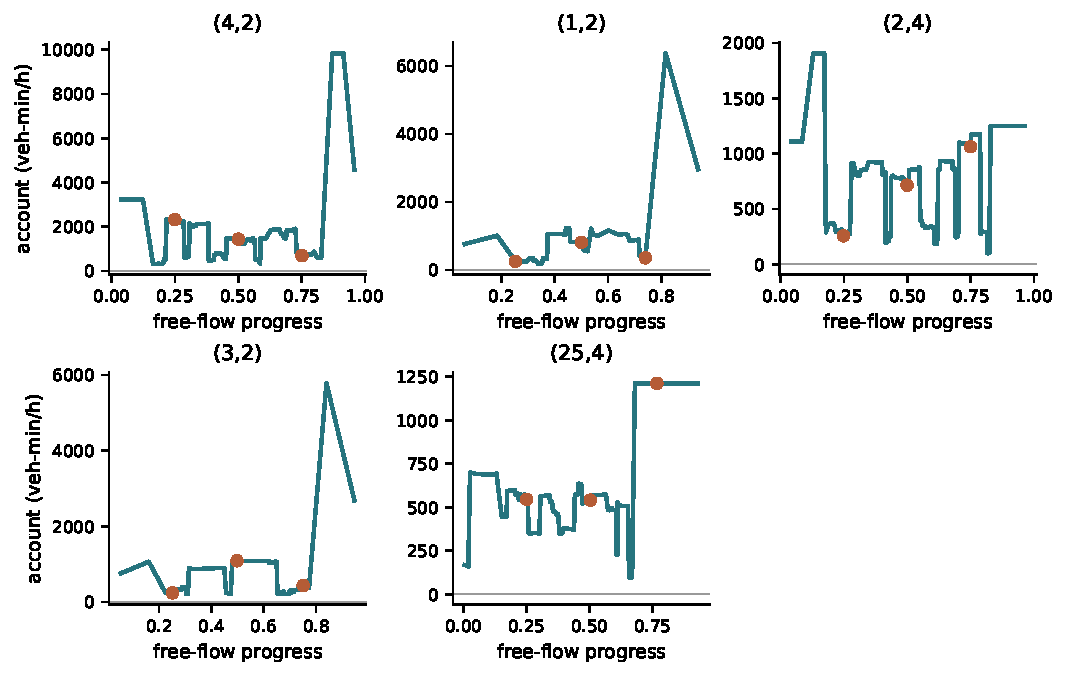
\includegraphics[width=0.99\linewidth]{../figures/fig_v108_anaheim_rest.pdf}
\caption{Anaheim spatial response profiles of the remaining five study
queries over the distance-based families: the attribution versus network-distance
progress along each query's own OD direction, with ochre dots marking
the three prespecified positions. All stay positive; family ranges span
roughly one to one and a half orders of magnitude.}\label{fig:anaheimrest}
\end{figure}
\begin{table}[pos=htbp]\centering\footnotesize\caption{Anaheim attributions over the complete distance-based family, with the three prespecified positions (vehicle-minutes per hour). Column heads are the prespecified targets; the exact selected levels are (row order) $0.250/0.501/0.752$, $0.252/0.500/0.740$, $0.248/0.499/0.750$, $0.251/0.498/0.751$, $0.251/0.504/0.768$ and $0.250/0.500/0.724$.}\label{tab:anaheim}\begin{tabular}{lrrrrrrr}\toprule OD & System & Unrestricted range & Family range & Regions & $\phi(0.25)$ & $\phi(0.50)$ & $\phi(0.75)$\\\midrule
(4,2) & 34664.1 & [-12712.6,20514.0] & [307.5,9832.1] & 211 & 2323.5 & 1441.8 & 692.3\\
(1,2) & 16773.6 & [-6032.2,9762.0] & [172.7,6374.8] & 83 & 259.0 & 818.0 & 360.5\\
(2,4) & 12143.7 & [-4374.6,6733.0] & [98.7,1905.9] & 211 & 257.0 & 714.6 & 1061.8\\
(3,2) & 14706.7 & [-5613.8,9052.9] & [202.8,5777.4] & 157 & 236.2 & 1087.3 & 434.6\\
(25,4) & 6919.3 & [-1805.3,3091.8] & [96.8,1212.2] & 164 & 545.6 & 540.7 & 1212.2\\
(25,2) & 11445.9 & [-4157.3,6904.5] & [131.8,5751.2] & 84 & 801.5 & 412.0 & 5751.2\\
\bottomrule\end{tabular}\end{table}
\begin{table}[pos=htbp]\centering\footnotesize\caption{Anaheim differences between preselected early and late regions, split by free-flow and congestion weights and study and background responses (vehicle-minutes per hour).}\label{tab:anaheimmechanism}\begin{tabular}{lrrrrr}\toprule OD & Free-flow study & Free-flow background & Congestion study & Congestion background & Total\\\midrule
(4,2) & -416.91 & -8.53 & -1499.94 & 294.16 & -1631.21\\
(1,2) & 9.85 & 6.96 & 83.01 & 1.71 & 101.54\\
(2,4) & 312.07 & -65.41 & 667.06 & -108.90 & 804.83\\
(3,2) & 50.04 & 11.80 & 136.55 & 0.04 & 198.43\\
(25,4) & 47.28 & -40.11 & 666.28 & -6.89 & 666.56\\
(25,2) & -131.77 & -10.52 & 5102.23 & -10.15 & 4949.79\\
\bottomrule\end{tabular}\end{table}

\begin{table}[pos=htbp]\centering\footnotesize
\caption{Location layer of the $(25,2)$ case: the boundary at each
reported position, its crossing links, and the principal signed
attribution contributions (vehicle-minutes per hour; positive entries
add to the origin-side attribution). Regions contain the origin; the two
plateau endpoints share the attribution $5{,}751.2$ on link
$63\!\to\!62$, while their second crossing link differs ($87\!\to\!86$
at the start, $2\!\to\!87$ at the end, contributing $-0.0$ at
both).}\label{tab:anaheimcrossing}
\setlength{\tabcolsep}{4pt}
\begin{tabular*}{\tblwidth}{@{\extracolsep{\fill}}lrrrl}
\toprule
Position & Region & Crossing & Principal links & Attribution\\
(progress) & (nodes) & links & (from$\to$to, contribution) &\\
\midrule
Early $0.250$ & 231 & 34 & $269\!\to\!261$ $+550.5$;\ $271\!\to\!192$ $+163.9$ & $801.5$\\
Middle $0.500$ & 405 & 4 & $191\!\to\!190$ $+297.0$;\ $66\!\to\!65$ $+105.4$ & $412.0$\\
Plateau $0.724$--$0.818$ & 413--414 & 2 & $63\!\to\!62$ $+5{,}751.2$;\ ($87\!\to\!86$/$2\!\to\!87$ $-0.0$) & $5{,}751.2$\\
Destination $0.911$ & 415 & 2 & $62\!\to\!2$ $+2{,}673.1$;\ ($2\!\to\!87$ $-0.0$) & $2{,}673.1$\\
\bottomrule\end{tabular*}\end{table}

\subsection{Learning objectives and exact endpoint targets}\label{app:learning-objectives}
Equation~\eqref{eq:localboundarybound} suggests learning the reference's weighted demand response
where it affects spatial attributions. With training-only positive scales
$a_j$, the boundary term is
\begin{equation}
\mathcal L=\mathcal L_{\mathrm{flow}}+\lambda_J\mathcal L_{\mathrm{response}}
+\lambda_{\mathrm{cut}}\mathcal L_{\mathrm{boundary}},\qquad
\mathcal L_{\mathrm{boundary}}
=\frac1{NK}\sum_{q,j}\left[\frac{\mathcal K_j(h_j(q))}{a_j}\right]^2.
\label{eq:trainingobjective}
\end{equation}
The reference Jacobian is obtained from the existing implicit SUE
sensitivity system (Appendix~\ref{supp:sue}). The empirical study
compares six objectives under a shared continuation protocol
(Appendix~\ref{app:pairs-v102}): flow only; the unweighted response
$\|J_j^L-J_j^S\|$; the weighted response $\|D^LJ_j^L-D^SJ_j^S\|$ of
Eq.~\eqref{eq:coldecompmain}; the pointwise boundary seminorm
$\mathcal K_j(D^LJ_j^L-D^SJ_j^S)$ of Eq.~\eqref{eq:trainingobjective};
and the two endpoint objectives below.
Derivative supervision itself is established in Sobolev training
\citep{czarnecki2017sobolev}, including finite-difference derivative targets
\citep{yuan2022sobolev}; the network-derived target here selects the
part of weighted response error that changes boundary attributions.
A circulation in $\ker B$ is invisible to $\mathcal K_j$, so flow and
response losses remain necessary for the other attribution objectives.
The target matches the reference's actual response; it does not force
its true internal attribution divergence to zero or replace TSTT weights
with uniform weights. Equation~\eqref{eq:localboundarybound} is a path
inequality; finite training-point losses alone do not certify an entire
demand domain.


For the following finite-change statement, the outcome is explicitly separable:
\[
g(F)=(g_e(F_e))_{e\in E},\qquad T(F)=\sum_{e\in E}g_e(F_e).
\]
\begin{proposition}[exact finite-change boundary target]\label{prop:pairboundary}
Let $f^L,f^S$ and the edgewise outcome $g$ be continuously differentiable
on an open demand domain, and let $q^\pm=q\pm h e_j$ with their entire
segment in that domain. Put
\[
z_j^r=g(f^r(q^+))-g(f^r(q^-)),\qquad r\in\{L,S\}.
\]
For the attribution of this single-OD change,
\begin{equation}
\max_{U:s_j\in U,\ t_j\notin U}|\phi_j^L(U)-\phi_j^S(U)|
=\mathcal K_j(z_j^L-z_j^S).\label{eq:pairboundaryexact}
\end{equation}
If all sufficiently small single-coordinate changes have matching
one common value on every separating boundary at every point of the domain,
then $BD^LJ_j^L=BD^SJ_j^S$ throughout the domain. Integrating yields
matching boundary attribution columns for any joint demand path in that
domain (with the same columnwise path convention).
\end{proposition}
Appendix~\ref{app:pairproof} proves both statements. The first is an
exact finite-change target, whereas the pointwise response objective
optimizes the upper bound in Eq.~\eqref{eq:localboundarybound}; integrating
before taking $\mathcal K_j$ can retain cancellations. The second statement
requires a domain-wide local premise and is not a guarantee from finite
training data. With several ODs changing, the endpoint outcome difference
only identifies the sum of their attribution columns.

For sampled single-OD endpoint pairs, a direct training objective is
\begin{equation}
\mathcal L_{\mathrm{pair}}=\mathcal L_{\mathrm{flow}}
+\lambda_{\mathrm{edge}}\frac1N\sum_{(q,h,j)}
\frac{\|z_j^L-z_j^S\|_2^2}{b_j^2}
+\lambda_{\mathrm{cut}}\frac1N\sum_{(q,h,j)}
\left[\frac{\mathcal K_j(z_j^L-z_j^S)}{a_j}\right]^2,
\label{eq:pairobjective}
\end{equation}
with positive training-only scales $a_j,b_j$. The edge term controls
changes invisible to the boundary seminorm, whose kernel is $\ker B$.
Two reference endpoint equilibria supply $z_j^S$; training uses ordinary
parameter backpropagation through two predictions, without reference
Jacobian labels or input-Jacobian differentiation.

\subsection{Learned-model evaluation protocol}\label{app:pairs-v102}
Six objectives continue each of five common conservative models for
1,200 Adam updates, with learning rate $3\times10^{-5}$, flow batch 32
and query batch eight. The flow data and seed-specific minibatch
sequences are shared. Each of six queries has 64 training and 16
validation endpoint pairs. Centers are sampled coordinatewise from
$[0.65,1.3]$ times baseline demand (seed 102111); half-widths 2.5\% and
15\% occur equally often. Only one demand changes per pair, while
background routes remain responsive.

The flow loss averages $[(f_e^L-F_e^S)/s_e]^2$ over minibatch states
and edges, with $s_e=0.01\sqrt{\operatorname{mean}_{\rm train}[(F_e^S)^2]}$ from the
2,500 training states. Each auxiliary objective adds one term
$\lambda\,\mathcal L_{\mathrm{aux}}$ to this flow loss, with the weight
grid $\lambda\in\{0.001,0.003,0.01,0.03,0.1,0.3,1\}$ searched
identically for every objective. Each normalizer carries the units of
its own target, so that the common grid explores comparable
regularization ranges: rescaling the outcome $T\mapsto cT$ rescales
the weighted terms' normalizers with them and leaves every effective
weight unchanged. With
$\langle\cdot\rangle_j$ denoting the average over query $j$'s training
centers or endpoint labels, the training-only scales are
\[
\begin{aligned}
u_j&=\max\{\sqrt{\langle\|J_j^S\|_2^2\rangle_j},10^{-6}\},&
v_j&=\max\{\sqrt{\langle\|D^SJ_j^S\|_2^2\rangle_j},10^{-6}\},&
b_j&=\max\{\sqrt{\langle\|z_j^S\|_2^2\rangle_j},10^{-6}\},\\
a_j&=\max\{\sqrt{\langle\mathcal K_j(z_j^S)^2\rangle_j},10^{-6}\},&
\bar a_j&=\max\{\sqrt{\langle\mathcal K_j(D^SJ_j^S)^2\rangle_j},10^{-6}\}.
\end{aligned}
\]
The auxiliary terms are: unweighted response
$\langle\|J_j^L-J_j^S\|_2^2/u_j^2\rangle$; weighted response
$\langle\|D^LJ_j^L-D^SJ_j^S\|_2^2/v_j^2\rangle$, with
$D^r=\operatorname{diag}(\nabla T(F^r))$ the outcome-gradient weights
of Eq.~\eqref{eq:Cdef} evaluated at each model's own flows (TSTT:
$\nabla_eT=t_e+F_et'_e(F_e)=t_{0,e}[1+0.75(F_e/c_e)^4]$);
the pointwise boundary seminorm
$\langle[\mathcal K_j(D^LJ_j^L-D^SJ_j^S)/\bar a_j]^2\rangle$; the
endpoint-edge term
$\langle\|z_j^L-z_j^S\|_2^2/b_j^2\rangle$; and the endpoint-cut bundle,
which adds $0.01$ times
$\langle[\mathcal K_j(z_j^L-z_j^S)/a_j]^2\rangle$ to the endpoint-edge
term (a fixed $0.01$ inner ratio, not an independently tuned
objective). The three
response-family objectives share one set of derivative labels; the two
endpoint objectives share one set of endpoint labels. The weighted
objective is run at every grid weight under this own-scale
normalization from the shared initializations.

Checkpoint selection uses one uniform rule for every objective and
weight: among the common initial model (update zero) and every 100th
continuation update whose validation flow error is at most $1.1$ times
the initial model's value, take the minimum validation boundary
mean-square error, using the same 96 validation pairs throughout. The
initial model ensures the pool is never empty. The weight $\lambda^*$ of
each objective is then chosen on validation data only: among the grid
values whose seed-median selected validation flow error stays within
$1.1$ times the seed-median initial error, minimize the seed-median
validation boundary error. The flow-only control reuses the flow
continuation under the same uniform rule. Test paths never enter
selection or weight choice. The extended-budget replication of
Section~\ref{sec:pairresults} repeats the response and flow
continuations with 3{,}600 updates under this unchanged protocol
(per-network costs in Appendix~\ref{app:anaheimlearning}).

The final evaluation uses 96 fixed test paths, all generated by one
rule: for each active-query group $k\in\{1,2,3,6\}$, draw a base state
uniformly from $[0.65,1.3]$ times baseline demand, choose the $k$
active queries in round-robin order, add independent changes of
$15$--$30\%$ of their baseline demands with alternating same-direction
and mixed-direction signs, and solve all 41 states of the resulting
straight demand path. Twenty-four paths (six per group, seed 102112)
and seventy-two paths (eighteen per group, seed 102113) were generated;
models and validation choices were fixed before evaluation on the
additional paths. For every path, flow error first averages relative
Euclidean errors across its states. Attribution statistics average active
queries and seeds within each path and then take medians across the 96 paths;
seeds do not add independent paths. For column error $e_j$ and reference column
$c_j$, relative column, system and unrestricted-boundary errors divide
$\|e_j\|_2$, $|\mathbf1^\top e_j|$ and $\mathcal K_j(e_j)$ by the
corresponding reference values, with absolute floor $10^{-6}$. Geometric error
uses $\max_{U\in\mathcal F_j^{\rm geo}}|\mathbf1_U^\top Be_j|$ and
the same maximum for $c_j$. Percentages multiply ratios by 100. The
incremental-flow error at the path endpoints is
$\norm{[f^L(q^1)-f^L(q^0)]-[f^S(q^1)-f^S(q^0)]}_2/\norm{f^S(q^1)-f^S(q^0)}_2$,
reported with the absolute numerator because the reference increment
is small relative to total flows (per path--seed medians of both, and
the smallest reference increment, in
Appendix~\ref{supp:learningdetail}).

The decomposition in Eq.~\eqref{eq:coldecomp} is evaluated at the same 41 states
with the same quadrature. Component norms describe error mechanisms; cancellation
prevents treating their norms as additive shares. The fixed-screenline sign
comparison in Appendix~\ref{supp:screenlinelearned} uses the separate
pre-specified six-query baseline segment and is not pooled with these 24 paths.
Table~\ref{tab:learning-costs} reports the incremental computation
costs of training-label generation, common validation and explanation
timing under the shared CPU protocol.
\begin{table}[t]\centering\footnotesize
\caption{Incremental computation costs (seconds) under the shared
continuation protocol. Training-label and common-validation costs are
measured separately on the same CPU protocol; training times are
continuation-time medians over the weight grid and seeds, and
explanation times are sequential medians for the selected models over
the 24-path timing subset defined below (totals for that subset).}
\label{tab:learning-costs}
\begin{tabular}{lrrrr}\toprule Labels & Training labels & Common validation & Continuation & Explanation\\\midrule
Flow only & 0.00 & 6.45 & 246.0 & 7.34\\
Response family & 16.12 & 6.45 & 155--425 & 7.13\\
Endpoint (edge, cut) & 25.75 & 6.45 & 441--497 & 7.27--7.59\\
\bottomrule\end{tabular}\end{table}
Training labels comprise 768 endpoint states for either endpoint
objective, or 384 center states and their sensitivities for the three
response-family objectives (unweighted, weighted, boundary-seminorm),
which share one label set. Every method additionally uses the same 192
endpoint states for validation; unused center-validation derivatives
are excluded. Existing flow data, pretrained models and the common test
reference are excluded from these incremental costs. The 984 test
states and sensitivities took 74.4\,s in the reference run.
Explanation timing covers a 24-path timing subset of the 96 test paths
(the seed-102112 paths, six per active-query group; forward
evaluation, six directional derivatives per state, quadrature and node
aggregation, excluding model loading): the table entries are totals
over that subset, about $0.3$\,s per path, not the full 96-path
evaluation. Continuation times include
initialization, validation and saving under concurrent jobs, pooled
across the original run and the renormalized-weight re-run under
lighter load; they describe the actual training expense and do not
establish a method speed advantage.


\paragraph{Out-of-domain evaluation.}
The two out-of-domain bands of Section~\ref{sec:pairresults}
(low loads on $[0.40,0.60]$ and high loads on $[1.35,1.55]$ times the
base vector) reuse the test-path generator unchanged --- 24 paths per
band, active-query groups $k\in\{1,2,3,6\}$ with six replicates,
deltas drawn from $U[0.15,0.30]$ times the base values with odd
replicates flipping every even-indexed delta, fresh seeds --- with
reference SUE flows and sensitivities at the same $41$-state
quadrature; the frozen flow and response checkpoints are evaluated
without retraining. The unrestricted metric compares the closed-form
node-divergence extrema of the learned and reference columns,
normalized by the reference unrestricted span.

\subsection{Conservation mechanism ablation}\label{app:conservation}
This experiment compares ways of obtaining flow conservation on
Sioux Falls under otherwise identical supervision, asking what the
conservative parameterization of Eq.~\eqref{eq:consparam} contributes
beyond conservation itself:
(i)~\emph{exact} --- the path-share parameterization, pretrained on the
unscaled flow loss (the published five-seed models of
Section~\ref{sec:pairresults});
(ii)~\emph{exact (scaled)} --- the same architecture pretrained on the
per-link scaled loss, the one recipe difference of the earlier
three-way comparison, removed by training the exact parameterization
on the direct models' objective;
(iii)~\emph{penalty} --- a direct MLP on link flows with a squared
node-balance penalty (weight $1$, normalized by the nodal-throughput
RMS over the training states, floored at the network average);
(iv)~\emph{projection} --- the same direct MLP whose output is
projected each step onto $\{f:Bf=Mq+b\}$ by the differentiable
least-norm map $f\mapsto f-B^{\!\top}(BB^{\!\top})^{\dagger}(Bf-Mq-b)$
(Moore--Penrose inverse; $BB^{\!\top}$ is singular for a connected
network). The direct-MLP width is solved from the parameter-count
equation so that all four models have $714{,}979$ parameters against
the exact model's $715{,}040$. Pretraining shares the data, optimizer
(Adam $3\times10^{-3}$, batch 256, at most 12{,}000 steps) and the
min-validation checkpoint rule (validation metric: unscaled relative
L2 flow error) across all architectures; the loss differs only as
stated. Continuation follows the protocol of
Appendix~\ref{app:pairs-v102} unchanged (1{,}200 updates, shared
labels and minibatch sequences, the uniform selection rule including
the pre-trained initial model in the candidate pool), with flow-only
and response supervision for each mechanism. The exact rows reproduce
the published five-seed medians exactly ($21.18\%$ and $14.19\%$
column error), and every projection output satisfies $Bf=Mq+b$ to
$2\times10^{-11}$; the path-share construction holds node balance to
the same scale under both pretraining losses.

\begin{table}[pos=htbp]\centering\footnotesize
\caption{Conservation mechanism ablation on the 96 Sioux Falls test
paths (medians of path-level values; active queries and seeds averaged
within path). Mechanisms: path-share parameterization under the two
pretraining losses, and the two direct mechanisms under the scaled
loss. Residuals are per-query maxima over the path states, maximized
over queries: the node-balance residual $\max_q\|Bf(q)-Mq-b\|_\infty$
(veh/h); the derivative residual
$\max_{q,j}\|\partial_j[Bf](q)-\mu_j\|_\infty/\|\mu_j\|_2$. Column:
attribution column error; incremental: endpoint flow-change error;
$E_{\mathrm{total}}$: normalized end-to-end summary error.}\label{tab:conservation}
\setlength{\tabcolsep}{3.6pt}
\begin{tabular*}{\tblwidth}{@{\extracolsep{\fill}}llrrrrrr}
\toprule
Mechanism & Method & Flow (\%) & Incremental (\%) & Node resid. & Deriv.\ resid. & Column (\%) & $E_{\mathrm{total}}$\\
\midrule
Exact & flow & 0.032 & 5.03 & $3\times10^{-11}$ & $9\times10^{-16}$ & 21.18 & 11.35\\
Exact & response & 0.029 & 3.52 & $3\times10^{-11}$ & $8\times10^{-16}$ & 14.19 & 8.68\\
\addlinespace
Exact (scaled) & flow & 0.033 & 5.53 & $3\times10^{-11}$ & $8\times10^{-16}$ & 21.60 & 10.33\\
Exact (scaled) & response & 0.032 & 3.81 & $3\times10^{-11}$ & $8\times10^{-16}$ & 14.35 & 8.19\\
\addlinespace
Penalty & flow & 0.040 & 22.76 & 42.1 & 1.16 & 183.7 & 148.8\\
Penalty & response & 0.039 & 22.24 & 42.1 & 1.17 & 177.9 & 144.9\\
\addlinespace
Projection & flow & 0.026 & 14.54 & $2\times10^{-11}$ & $2\times10^{-15}$ & 104.1 & 46.4\\
Projection & response & 0.026 & 14.42 & $2\times10^{-11}$ & $2\times10^{-15}$ & 99.4 & 45.6\\
\bottomrule\end{tabular*}\end{table}

Table~\ref{tab:conservation} supports three readings. First, the
pretraining loss is not what separates the exact parameterization from
the direct mechanisms: under the same scaled loss the exact
architecture attains $21.60\%$ and $14.35\%$ column error against the
projection's $104.1\%$ and $99.4\%$, and training the exact
architecture on the scaled loss leaves its column errors within half a
percentage point of the published unscaled values ($21.18\%$,
$14.19\%$) while slightly lowering its end-to-end summary error. The
exact-versus-direct gap is therefore a property of the
parameterization, not of its training recipe. Second, conservation
itself still matters: the penalty model matches the flow accuracy of
the exact model ($0.040\%$) with a small output residual ($42$ veh/h
against nodal throughputs in the thousands), yet its integrated
attribution residual --- the quantity $R_j$ of
Eq.~\eqref{eq:residualidentity} --- reaches $0.66$ in units of the
demand-conservation scale $|\Delta q_j|\|\mu_j\|_2$, its derivative
balance residual is $1.16$ in the same normalization, and the
downstream outcome columns inherit the damage; the chain of
Eq.~\eqref{eq:residualidentity} is exactly what fails, because the
penalty controls $r(q)$ but not $\partial_jr$. The projection enforces
output conservation exactly and transfers it to derivatives and to the
integrated residual, cutting the column error to $104.1\%$ while
remaining far above the exact parameterization, because projecting an
unconstrained response field onto node balance does not reproduce the
path-share structure that the assignment imposes. Third, response
supervision improves every mechanism (penalty $183.7\to177.9$,
projection $104.1\to99.4$, exact $21.18\to14.19$ and
$21.60\to14.35$), with by far the largest effect inside the exact
parameterization: the inductive benefit of
conservation-by-construction and the statistical benefit of derivative
supervision are complementary rather than substitutes.

\subsection{Label-budget repetitions}\label{app:labelbudget}
The label-efficiency experiment of Section~\ref{sec:pairresults}
retrains response supervision at the selected weight with per-query
derivative-center budgets of $6$, $12$, $24$ and $48$ centers (36--288
in total against the full 384). Each budget uses three independent
query-balanced random nested subsets: for replication $\rho$ and query
$j$, a fresh permutation of that query's $64$ training centers is drawn
from $\mathrm{rng}(20261101+\rho+97j)$, and the budget-$b$ subset is
the first $b$ entries, so the subsets of different budgets nest within
a replication while different replications are independent. Training
follows the continuation protocol of Appendix~\ref{app:pairs-v102}
unchanged (shared flow data and minibatch sequence, 1{,}200 updates,
uniform selection rule); only the derivative-label pool shrinks. The
reported curves aggregate hierarchically: within each subset
replication, the median over the 96 test paths; across the three
replications, the median of those three medians, with the shaded band
spanning their interquartile range. The full-budget point (384
centers) is the single run with the complete label set and carries no
subset variation. Across all budgets the interquartile range
stays within $0.8$ percentage points for the column error and within
$0.4$ for the family-boundary error, and flow accuracy stays within
$0.027$--$0.031\%$.

\begin{figure}[t]
\centering
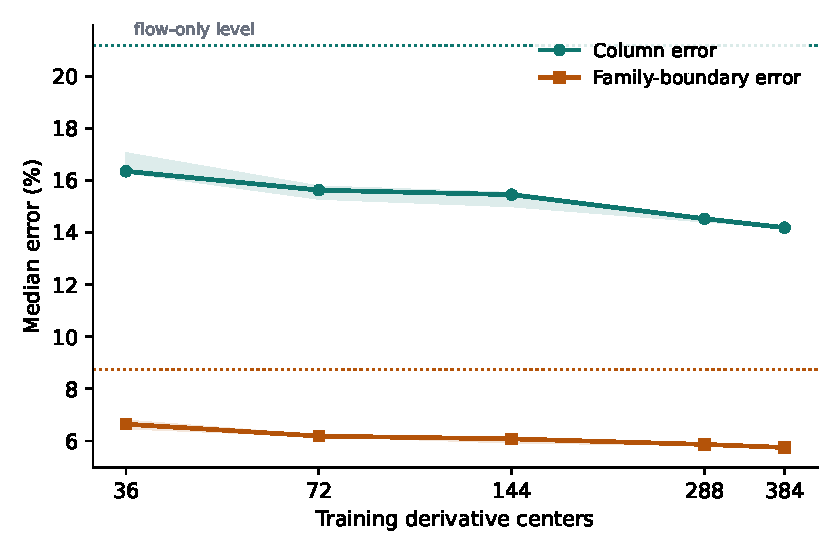
\includegraphics[width=0.72\linewidth]{../figures/fig_v111_labelbudget.pdf}
\caption{Response supervision under reduced label budgets on the 96
test paths, at the validation-selected weight: median attribution
column and family-boundary errors against the number of training
derivative centers (36--384; logarithmic axis), aggregated as stated
above (shaded: interquartile range over the three subset replications;
the 384-center point is the single full-label run), with the flow-only
levels marked (dotted).}\label{fig:v109labelbudget}
\end{figure}

\section{Numerical accuracy and supporting results}\label{supp:numdetail}\label{supp:transrecords}
\subsection{Grid refinement, derivative, and solver checks}\label{supp:accuracy}
All differences here are observed numerical comparisons, not certified
bounds. Direct attribution-column differences are at most 0.178\% for
11 versus 41 states and $1.1\times10^{-4}\%$ for six-query/single-OD
41 versus 81 states. Near-zero attributions on 41/81/161 grids change by
less than $5\times10^{-6}$ percentage points (absolute $<0.01$); the
learned 201/801-state relative difference is $4.97\times10^{-6}$.
Implicit versus re-solved central-difference Jacobian errors are at most
$7.6\times10^{-5}$ (halved step $2.5\times10^{-5}$), or
$3.0\times10^{-8}$ for six-query/single-OD columns. Newton versus
successive-averages differences over 1,353 solves are at most
$1.31\times10^{-11}$. Maximum fixed-point and balance residuals are
$3.10\times10^{-8}$ and $1.82\times10^{-11}$ veh/h. Scalar completeness
relative discrepancies are at most $3.36\times10^{-5}$ for
frozen- and responsive-background settings and $1.9\times10^{-7}$ for single-OD checks.
Per-edge endpoint checks give relative column errors
$7.7\times10^{-8}$--$1.1\times10^{-6}$ and maximum entry residuals
$5.4\times10^{-4}$--$1.6\times10^{-2}$ TSTT units. Per-query records
remain in the arrays. The direct $(10,16)$ attribution change is 24.80\%
on its 41-state grid; Figure~\ref{fig:respfield} uses the seed-zero
learned model on 201 states (24.8\%). On the same realized response,
the active-link outcome $T(F)=F_{10\to16}$ balances exactly in the OD
direction on the single selected arc while its scale depends on the
circulation --- the directional balance of
Section~\ref{sec:levels} without a response-independent boundary value.

\subsection{Normalization, cancellation, and sensitivity}\label{supp:additional}
Every OD of the background-treatment comparison of
Section~\ref{sec:variation} appears in
Tables~\ref{tab:bgfull} and~\ref{tab:cutspreadfull}: the learned
zero-background unrestricted ratios of the three most divergent queries
$(17,10)$, $(16,10)$ and $(11,10)$ are $59.71\%$ ($58.92$--$61.23$ over
seeds), $36.80\%$ ($36.41$--$38.40$) and $0.18\%$ ($0.03$--$0.27$),
closely tracking the direct-SUE values.

\begin{figure}[pos=tb]
\centering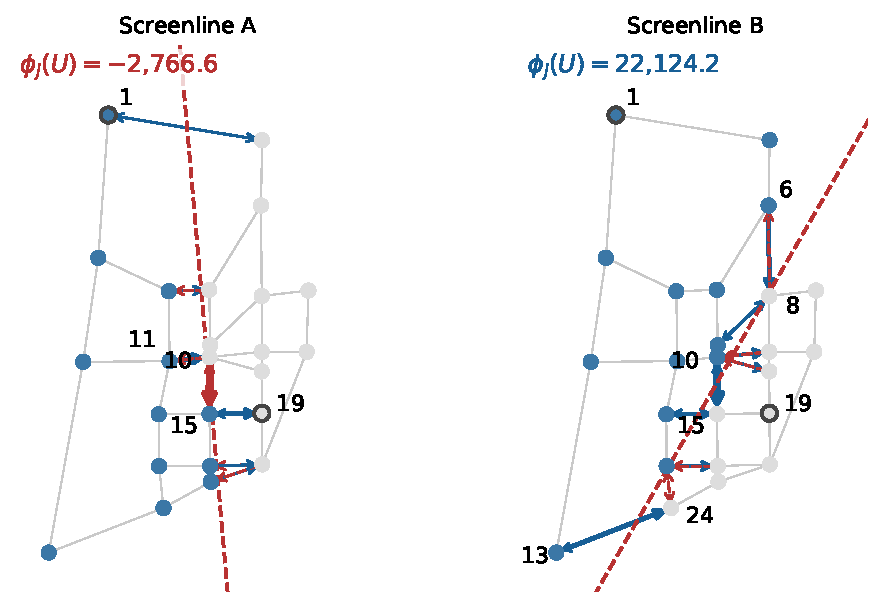
\includegraphics[width=0.66\linewidth]{../figures/fig_screenlines_v109.pdf}
\caption{Contrasting screenline attributions for the same positive OD
contribution. Two straight screenlines for OD $(1,19)$ under the
responsive-background assignment. Blue nodes belong to $U$; gray nodes
are outside; dashed lines separate the two sides. Node $1$ is inside
and node $19$ outside in both panels. The two lines have different
normal directions, so they are labeled Screenline~A (left) and
Screenline~B (right); the crossing progress of each with the straight
origin--destination segment is $0.61$ and $0.78$, an ordering of the
crossing positions that does not by itself make the two enclosed
regions nested. The two boundary attributions have opposite signs while the
network-wide contribution is positive; arrows encode the signed
crossing contributions (solid blue = positive, dashed red = negative,
width = magnitude). Principal crossing contributions, Screenline~A:
$10\to15$ $-9195.2$, $11\to10$ $+3169.6$, $15\to19$ $+2689.9$;
Screenline~B: $10\to15$ $+9195.2$, $13\to24$ $+3602.1$, $6\to8$
$+3508.8$ (TSTT units). The lines are the minimum and maximum of the
prespecified geometric family; the complete irregular connected minimum
and its crossing-link decomposition appear in
Figure~\ref{fig:negmech}.}
\label{fig:screenlines}\end{figure}
\paragraph{Complete cut-range records.}
Table~\ref{tab:cutspreadfull} reports the complete eight-OD records of
the responsive-background treatment (all demands at published values,
all routes re-equilibrated; $41$ quadrature points, implicit
sensitivities): connected regions retain $60.41$--$76.85\%$ of the
unrestricted range on every OD, and the per-query ordering of the
learned zero-background ratios above is retained. The two auxiliary
treatments of Section~\ref{sec:variation} are complete in
Table~\ref{tab:bgfull}: zero background removes most of the spread of
the three queries that rerouting later amplifies, and the frozen
background sits between the two.
\begin{table}[pos=htbp]\centering\footnotesize
\caption{Complete eight-OD unrestricted cut ranges (percent of each
attribution's absolute origin-cut value) under the two auxiliary
background treatments. A: zero background (direct logit-SUE, $41$
quadrature points); B: background link flows frozen at the joint
baseline equilibrium (study-only re-solve, $11$-point chain, the
protocol of the frozen-flow check).}\label{tab:bgfull}
\small
\begin{tabular*}{\tblwidth}{@{\extracolsep{\fill}}lrrrrrrrr}
\toprule
& \multicolumn{8}{c}{OD}\\
\cmidrule(lr){2-9}
Treatment & $10{\to}16$ & $16{\to}10$ & $10{\to}11$ & $10{\to}15$ & $15{\to}10$ & $10{\to}17$ & $11{\to}10$ & $17{\to}10$\\
\midrule
A: zero background (\%) & 26.94 & 36.86 & 0.0075 & 0.77 & 0.77 & 37.48 & 0.0073 & 59.95 \\
B: frozen background (\%) & 34.18 & 40.24 & 1.26 & 19.01 & 22.13 & 43.71 & 0.87 & 56.52 \\
\bottomrule
\end{tabular*}
\end{table}
\begin{table}[pos=htbp]\centering\footnotesize
\caption{Complete eight-OD cut ranges under the responsive-background
treatment: unrestricted and connected-family ranges as percentages of
each attribution's absolute origin-cut value, the
connected-to-unrestricted ratio, and the number of enumerated connected
regions. Direct SUE, $41$ quadrature points, implicit
sensitivities.}\label{tab:cutspreadfull}
\small
\begin{tabular*}{\tblwidth}{@{\extracolsep{\fill}}lrrrr}
\toprule
OD & Unrestricted range (\%) & Connected (\%) & Ratio (\%) & Regions\\
\midrule
$10\to16$ & $109.04$ & $83.80$ & $76.85$ & 13{,}253\\
$16\to10$ & $166.26$ & $127.72$ & $76.82$ & 13{,}253\\
$10\to11$ & $84.67$ & $51.27$ & $60.56$ & 10{,}270\\
$11\to10$ & $81.09$ & $48.98$ & $60.41$ & 10{,}270\\
$10\to15$ & $71.88$ & $49.90$ & $69.42$ & 11{,}182\\
$15\to10$ & $84.05$ & $58.24$ & $69.29$ & 11{,}182\\
$10\to17$ & $49.11$ & $31.57$ & $64.27$ & 11{,}482\\
$17\to10$ & $54.77$ & $35.27$ & $64.39$ & 11{,}482\\
\bottomrule
\end{tabular*}
\end{table}
\paragraph{Error-metric definitions.}
The surrogate test flow error is, within each seed, the mean over the
$857$ test demands of
$\|f(q)-F^{\mathrm{SUE}}(q)\|_2/\|F^{\mathrm{SUE}}(q)\|_2$, reported
as the median over the five seeds; Jacobian column errors
$\|J_j^{\mathrm{learned}}-J_j^{\mathrm{SUE}}\|_2/\|J_j^{\mathrm{SUE}}\|_2$
are pooled over the $5\times41\times8$ seed--point--OD columns;
attribution-column errors use the per-column norm over the $40$
seed--OD columns on the common $41$-point grid.

\paragraph{Same-path flow, sensitivity, and boundary-attribution errors.}
The test-split flow error is not paired with the Jacobian comparison;
re-summarized on the same $41$ zero-background quadrature points for
each seed, flow error is $0.136\%$ (median; $1.331\%$ maximum),
Jacobian column error $0.516\%$ ($9.562\%$ maximum), attribution-column
error $0.349\%$ ($1.80\%$ maximum), and the connected-boundary error
$E_j^{\mathrm{cut}}$ $0.204\%$ ($1.739\%$ maximum; largest errors at
OD $(16,10)$, seed $3$). The per-query absolute origin-cut
denominators behind Tables~\ref{tab:bgfull}
and~\ref{tab:cutspreadfull}, the responsive-background
link-sum comparison ($C_j$ spanning $2.078$--$4.282\times10^5$ TSTT
units, $1.01$--$2.37$ times the origin-cut attributions, endpoint
completeness within $2.3\times10^{-5}$ relative) and the node-level
study/background divergence breakdown behind
Section~\ref{subsec:bgsplit} accompany the result arrays in the code
package.

For the learned zero-background low-range group, five-seed median pointwise
imbalance budgets $100A_j/|\phi_j(\{s_j\})|$ lie between $0.22\%$ and
$0.95\%$, versus $26.85$--$59.71\%$ for the high group; the low-group
median cancellation factors are at most $0.313$ (one seed reaches
$\kappa=0.852$), so small pointwise imbalance mainly limits the
low-group range, while the high group's median $\kappa$ is below
$8\times10^{-5}$.

Zero-background route-choice dispersion checks at $\theta\in\{0.5,1,2\}$
(eleven-point direct-SUE calculations) retain the large/small
separation --- large ranges $27$--$64\%$, the others below $9.4\%$.

\subsection{Full-background six-query surrogate validation}\label{supp:fullbgsurrogate}
The six-query study model shares the conservative parameterization of
Appendix~\ref{supp:protocol} with a full $5{,}280$-path head: the input
is the six-dimensional study demand vector (the other $522$ ODs stay
at published demand), $z$ is the same $3\times128$ tanh MLP on
standardized demands, and $f=\Delta h$ conserves exactly by
construction. It is pretrained flow-only under the same sampling
principle as the zero-background surrogate (the six study demands
scaled by i.i.d.\ LogNormal$(0,0.5^2)$ factors clipped to $[0.2,2]$,
$2500/857/857$ split; unscaled MSE; Adam at $3\times10^{-3}$,
minibatch $256$, at most $12{,}000$ steps, validation every $50$), and
the minimum-validation checkpoint of each seed $0,\ldots,4$ supplies
the five common initial models continued by every objective of
Section~\ref{sec:pairresults}; the test split enters only final
reporting. This flow-only model already reaches held-out flow errors
of $0.040\%$ (seed median) while its attribution-column errors remain
large (medians $7.4$--$81.2\%$ across the six queries): accurate flows
do not by themselves yield accurate spatial explanations --- the
observation that motivates the response-supervised protocol. The
two-term split of Eq.~\eqref{eq:coldecomp} locates this error in the
response term; complete validation records, conservation residuals and
across-seed envelopes are included in the released result arrays.

\subsection{Sensitivity to candidate paths and route-choice dispersion}\label{supp:coverage}
The path-set comparison expands all $528$ OD sets to twenty
candidates each (the first ten unchanged), with demands, BPR
functions, $\theta=1$, and $41$ quadrature points fixed: across the
eight queries, absolute unrestricted and connected ranges change by
at most $0.977\%$ and $1.011\%$, with the three largest
internal-node terms keeping their ordered node IDs (moving at most
$1.43\%$). The $\theta\in\{0.5,2\}$ check splits the specified
$(10,16)$ boundary difference into study/background components
$-7{,}404.9$/$-2{,}371.5$ at $\theta=0.5$ and $+115.3$/$+235.7$ at
$\theta=2$; these are different fixed-path models, not convergence to
unrestricted SUE. For all three additional models, implicit derivative
columns match re-solved half-step central differences at the
demand-path midpoint (maximum $0.00249\%$, completeness gap
$2.85\times10^{-5}$).

\subsection{Six-query interval, mechanism, boundary-family, and
scenario checks}\label{supp:newodaccuracy}


\textbf{Extremal ranges and negative shares.}
Unrestricted extrema follow the closed form \eqref{eq:cutextrema},
connected extrema the same enumeration as the connected ranges; the
negative shares in Section~\ref{subsec:newod} are exact counts over
the connected families ($4{,}621$--$16{,}943$ admissible sets per
query), and all displayed values come from the $41$-point columns.
Scenario robustness: under twenty candidate paths, $\theta\in\{0.5,2\}$
and the single-OD $0.2\to1.6$ re-run, the connected ranges of the
three sign-crossing queries move by at most a few percent (e.g.\ for
$(1,19)$, the connected range moves from the ten-path baseline
$[-13{,}502,\ 24{,}260]$ to $[-13{,}451,\ 24{,}276]$ under twenty
paths, and to $[-13{,}024,\ 24{,}064]$ at ten paths under
$\theta=0.5$; unrestricted intervals within $1\%$ of the baseline
row), and the single-OD
small-interval bands narrow to $[-1{,}947,\ 3{,}494]$, $[-1{,}201,\
5{,}838]$ and $[-2{,}517,\ 8{,}608]$ at $\pm10\%$ with every $C_j$
positive ($+7{,}202$ to $+33{,}734$; the control $(6,8)$ stays
sign-consistent throughout). The complete range table accompanies the
result arrays.
Table~\ref{tab:negmech} reports, for each sign-crossing query, the
connected minimizing boundary $U_-$ at the baseline setting: its
attribution, and the interior divergence sum
$\phi_j(\{s_j\})-\phi_j(U_-)$, decomposed as the table caption
specifies, at the same joint state and gradient as the reported
columns (additivity $\le1.2\times10^{-10}$).
By Eq.~\eqref{eq:cutgap}, the negative divergence captured inside
$U_-$ ($4{,}664.9$, $6{,}960.1$, and $19{,}811.5$ for the three
queries) covers $83\%$, $88\%$, and $72\%$ of the gaps
$\phi_j(U_-)-\phi_j^{\min}$, while the captured positive divergence
($19{,}938.0$, $18{,}194.2$, $46{,}901.4$) is $95.5\%$, $94.8\%$,
and $85.7\%$ of the query totals. The sign change arises
differently across queries: study response
dominates for $(1,19)$ (largest node $15$: own $+14{,}464.0$),
study- and background-dominated nodes share the sign for $(1,15)$,
and both contribute about equally for $(7,12)$ (node $8$). The
extremal node sets $U_-$ and $U_+$ (one-based node IDs; $U_-(1,19)$
is the shaded region of Figure~\ref{fig:negmech}) accompany the
result arrays.

\begin{table}[pos=tbh]
\footnotesize
\caption{Connected minimizing boundary $U_-$ at the baseline setting
for the three sign-crossing queries, in TSTT units. Interior is the
divergence sum over $U_-\setminus\{s_j\}$, decomposed into the query's
own response, the other five query ODs, and the background response;
the study group of the main text is the sum of the first two columns.
Entries are rounded independently.}
\label{tab:negmech}
\small
\begin{tabular*}{\tblwidth}{@{\extracolsep{\fill}}lrrrrrr}
\toprule
OD & $\phi_j(\{s_j\})$ & $\phi_j(U_-)$ & Interior & Own OD & Other query & Background\\
\midrule
$(1,19)$ & $1{,}771.6$ & $-13{,}501.6$ & $15{,}273.1$ & $19{,}480.9$ & $-59.4$ & $-4{,}148.3$ \\
$(1,15)$ & $2{,}948.1$ & $-8{,}286.0$ & $11{,}234.1$ & $7{,}856.9$ & $-26.7$ & $3{,}404.0$ \\
$(7,12)$ & $9{,}473.8$ & $-17{,}616.2$ & $27{,}089.9$ & $14{,}002.3$ & $-3.2$ & $13{,}090.8$ \\
\bottomrule
\end{tabular*}
\end{table}

\textbf{Neighborhood families.}
Origin-centered families built from undirected hop distance or
shortest free-flow distance (attained radii, destination excluded,
two-sided connected) contain $4$--$14$ admissible sets per query and
have positive ranges with minima at the origin cut ($1{,}771.6$ to
$15{,}803.5$ for $(1,19)$, $2{,}948.1$ to $26{,}602.0$ for $(1,15)$,
$9{,}473.8$ to $32{,}139.4$ for $(7,12)$); for short-path queries
$(7,18)$, $(4,5)$ and $(6,8)$ only the origin cut is admissible.

\textbf{Straight screenlines.}
Coordinates use an equirectangular frame (longitude scaled by the cosine
of mean latitude). Section~\ref{sec:scan}'s 36-direction construction,
with duplicate regions removed, gives 35, 152, 32, 123, 23 and 148
regions in Table~\ref{tab:newod} order. All attributions agree with direct
incidence aggregation below $10^{-9}$. Refining directions from
$5^\circ$ to $1^\circ$ leaves both negative minima unchanged; negative
shares change from 1.3\% to 1.8\% for $(1,19)$ and 6.8\% to 6.2\%
for $(7,12)$. Other queries stay positive; only $(7,18)$'s minimum
changes, from 642.4 to 641.4.

\textbf{Model-setting and single-OD checks.}
Re-solving the protocol of Appendix~\ref{supp:newod} under twenty
candidate paths per OD, $\theta\in\{0.5,2\}$, and the single-OD
demand paths ($0.2\to1.6$ of published demand, one moving coordinate;
$C_j$ within $3.9\%$, staying positive at $50{,}322.2$,
$77{,}672.6$, $117{,}476.8$ for the three crossing queries) leaves
every crossing query's connected range straddling zero, with extrema
attained by exactly the joint-scenario sets $U_-$ and $U_+$ (changes
at most $0.9\%$ and $0.5\%$) and the control $(6,8)$
sign-consistent throughout; solver and finite-difference checks match
Appendix~\ref{supp:newod} levels, and the $41$-point check ($(1,19)$,
$0.8\to1.2$) reproduces the endpoint column to $1.3\times10^{-5}$
TSTT units per edge.

\begin{figure}[pos=htbp]
\centering
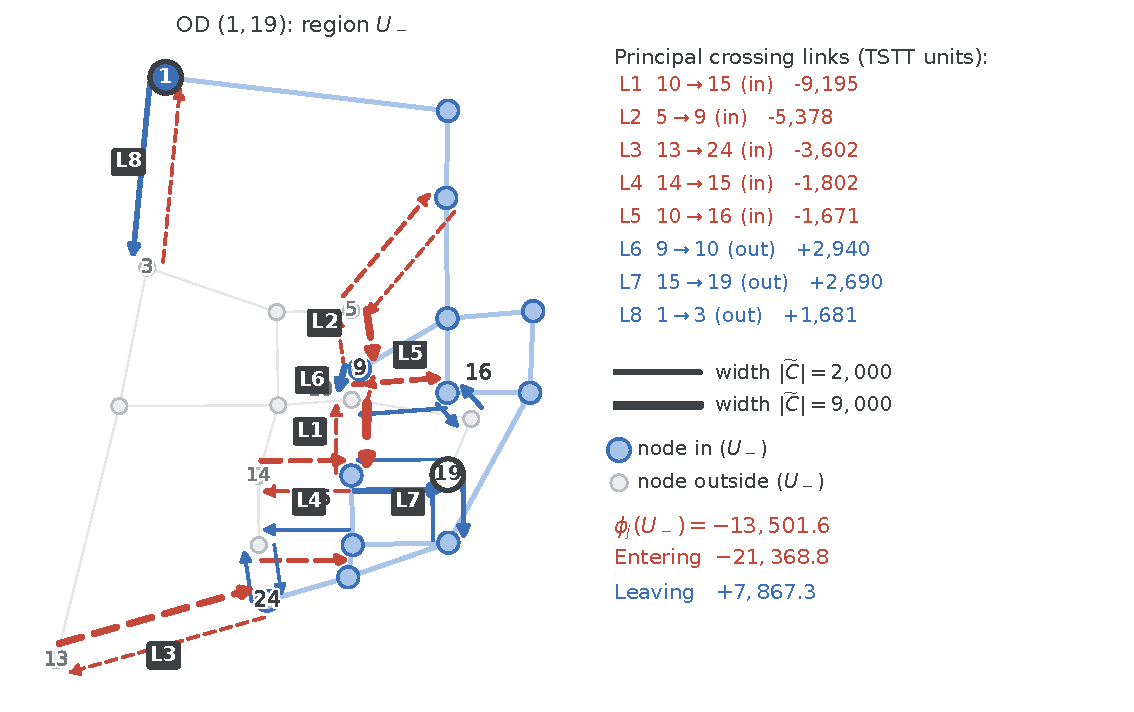
\includegraphics[width=0.82\linewidth]{../figures/fig_negmech_v102.pdf}
\caption{The connected minimizing region $U_-$ for OD $(1,19)$
(responsive-background six-query protocol). Shaded nodes form $U_-$ (origin
node $1$ ringed; destination $19$ outside). Crossing-link arrows keep
the link direction; width scales with $|c_{e,j}|$, and
color and style encode the signed contribution to $\phi_j(U_-)$,
$a_{e,j}=\sigma_ec_{e,j}$ ($\sigma_e=+1$ leaving, $-1$
entering; solid blue positive, dashed red negative), so a positive
attribution on an entering link appears red. The side panel lists, in
TSTT units, the five largest negative and three largest positive
contributions among the $26$ crossing links
($\mathrm{L}1$--$\mathrm{L}5$ negative, $\mathrm{L}6$--$\mathrm{L}8$
positive, ``(in)''/``(out)'' marking entering and leaving links),
with the width scale and the membership legend.}
\label{fig:negmech}
\end{figure}

\FloatBarrier
\subsection{Sign preservation on the six-query baseline segment}\label{supp:screenlinelearned}
On the six-query connected families, the five flow-supervised
pretrained models (Section~\ref{supp:protocol}) show five-seed median
largest-boundary disagreements of $4.2$--$6.9\%$ of the direct
connected span for four queries, rising to $99.5\%$ for the
small-response query $(4,5)$ and beyond the span for $(7,18)$ ---
flow-only supervision does not control boundary error. Sign reliability, by contrast, is boundary specific:
all five seeds retain the three connected-family sign crossings and
positive system contributions, and at the fixed direct-model minimizing
screenline every seed keeps the negative sign for $(1,19)$ and
$(7,12)$ (seed ranges $[-3886.6,-3365.1]$ and $[-2810.4,-1916.6]$
against references $-2766.6$ and $-2967.3$, with largest family-wide
errors below the reference sign margins). These are screenline-specific
certificates of sign preservation, not of column magnitudes; the
per-query screenline table and across-seed envelopes are included in
the released result arrays.

\subsection{Numerical diagnosis of the transferability hierarchy}\label{supp:levelsdiag}
The universal structural condition quantifies over all conservative
responses; Section~\ref{sec:levels} introduced the model-specific level
that reasons on the path-feasible response envelope of the assignment
model's fixed path sets.
Table~\ref{tab:levelsdiag} evaluates the hierarchy numerically. On the
Figure-1 network with its published post-merge weights, the universal
condition fails because the off-path pendant atom is heterogeneous, yet
the model-specific tests hold exactly for the all-simple-paths
structure: every rerouting that model can make preserves the common
boundary value, so restricting attention to the path-feasible envelope
restores transferability that the universal condition denies. On Sioux
Falls the two levels coincide --- the full-background fixed-path model
spans the complete circulation space through path exchanges, so its
path-feasible envelope contains every conservative response
(Appendix~\ref{supp:networks}) --- and both fail at realistic TSTT
weights, leaving the realized summaries of Table~\ref{tab:newod} as the
operative output. The diagnosis is stable across load levels: the
normalized universal violation stays within $2.08$--$2.21$ from the
$0.7$ to the $1.3$ baseline while $\rho_{\mathrm{swap}}$ falls from
$1.12$ to $0.80$ as congestion grows. On Anaheim the universal test
fails more decisively (normalized violation $10.08$) and the
model-specific test fails with it ($\rho_{\mathrm{swap}}=2.18$ over the
$404$-dimensional exchange space), so there too the realized layer
carries the reporting.

\begin{table}[t]\centering\footnotesize
\caption{Numerical diagnosis of the transferability hierarchy of
the four levels of Section~\ref{sec:levels}. $\eta_{\mathrm{all}}$ and
$\eta_{\mathrm{conn}}$: weight spread within all atoms / within the
queried atoms, normalized by the mean weight. $\rho_{\mathrm{swap}}$:
weighted-divergence leakage of unit rerouting directions relative to a
unit reference response; $\rho_{\mathrm{swap}}=0$ certifies
$BDN=0$, and together with zero off-span residuals
$\rho_{\mathrm{ref},j}$ it certifies both conditions of the
model-specific level. On Sioux Falls (level $1.0$) three of the six
queries have $\rho_{\mathrm{ref},j}=0$; the other three lie in
$0.83$--$0.97$. Realized: median
normalized geometric common-summary error of the responsive-background six
queries. Synthetic: published post-merge weights; Sioux Falls: TSTT
weights at the level-$1.0$ equilibrium, where the path-exchange space
attains the full circulation dimension $53$.}\label{tab:levelsdiag}
\begin{tabular}{lrrrr}\toprule
Network & $\eta_{\mathrm{all}}$ & $\eta_{\mathrm{conn}}$ & $\rho_{\mathrm{swap}}$ & Realized (\%)\\\midrule
Figure-1 synthetic & $0.61$ & $0$ & $0$ & $0$ (model responses)\\
Sioux Falls & $2.08$ & $=$ & $0.88$ & $32.3$\\
\bottomrule\end{tabular}\end{table}

\subsection{Additional learning comparisons}\label{app:legacy-learning}\label{app:learning-protocol}\label{app:calibration-protocol}
The attribution-column error of a learned model splits exactly into a
weight-shift and a response term ($L$/$S$: learned/direct in
Eq.~\eqref{eq:Cdef}):
\begin{equation}
c_j^{L}-c_j^{S}
=\Delta q_j\int_0^1(D_\lambda^{L}-D_\lambda^{S})J_j^{S}\,\mathrm{d}\lambda
+\Delta q_j\int_0^1D_\lambda^{L}(J_j^{L}-J_j^{S})\,\mathrm{d}\lambda,
\label{eq:coldecomp}
\end{equation}
satisfied entrywise within $10^{-10}$ TSTT units on the 96 test paths;
the weight-shift term has querywise median norm at most 0.2\% of the
reference column and the response term is larger in every seed--query
unit.

\paragraph{Six objectives under a fair weight search.}
Table~\ref{tab:fairmethods} completes the objective comparison under
the shared continuation budget and the common validation-only weight
search (Appendix~\ref{app:pairs-v102}). Each objective's auxiliary
term is normalized by a scale carrying that objective's own units ---
in particular the weighted-response term by its reference scale
$v_j^2=\langle\|D^SJ_j^S\|_2^2\rangle_j$ rather than the unweighted
scale --- so that a common weight grid explores comparable
regularization ranges; under this normalization every objective trains
at a properly selected weight. Weighted-response supervision reaches a
column error of $15.21\%$ at its selected weight, improves 84 of 96
paths, and trains across the whole low-to-mid weight range; the
unweighted form is the simplest member of the family and attains the
lowest errors on every metric. With validation-selected weights, both
endpoint objectives improve attribution accuracy relative to flow-only
training ($21.18\%\to16.2\%$ in column error), although their errors
remain above those of the response-supervised objectives. The
boundary-seminorm objective shows the largest validation--test gap:
its validation boundary error decreases monotonically with the weight
up to the selected $\lambda^*=0.3$ and reaches the lowest validation
value of any objective, yet its test column error at that weight stays
above flow-only training ($24.18\%$, improved on only 8 of 96 paths).
As Section~\ref{sec:pairresults} discusses through the seminorm
kernel, optimizing the boundary value alone does not repair the
underlying response field, whereas supervising that field improves
every spatial error metric.
\begin{table}[t]\centering\footnotesize
\caption{Six supervision objectives on the same 96 test demand paths,
each at its validation-selected weight $\lambda^*$ under the shared
continuation budget and uniform selection rule
(Appendix~\ref{app:pairs-v102}); the weighted-response objective is
normalized by its own reference scale $v_j$. Entries are medians of
path-level values; improved: paths on which the objective lowers the
column (family-boundary) error relative to flow-only
training.}\label{tab:fairmethods}
\setlength{\tabcolsep}{5pt}
\begin{tabular*}{\tblwidth}{@{\extracolsep{\fill}}lcccc cc}
\toprule
Objective & $\lambda^*$ & Flow pred.\ (\%) & Column (\%) & Family boundary (\%) & \multicolumn{2}{c}{Improved vs.\ flow}\\
\cmidrule(lr){6-7}
& & & & & col. & fam.\\
\midrule
Flow only & --- & 0.032 & 21.18 & 8.74 & --- & ---\\
Response supervision & 1 & 0.029 & 14.19 & 5.75 & 92/96 & 90/96\\
Weighted response & 0.1 & 0.032 & 15.21 & 6.93 & 84/96 & 79/96\\
Boundary seminorm & 0.3 & 0.037 & 24.18 & 7.21 & 8/96 & 45/96\\
Endpoint-edge & 0.3 & 0.035 & 16.23 & 7.46 & 72/96 & 66/96\\
\quad + cut term$^{\dag}$ & 0.3 & 0.035 & 16.26 & 7.47 & 72/96 & 67/96\\
\bottomrule\end{tabular*}\end{table}
\noindent$^{\dag}$The endpoint-cut bundle is the endpoint-edge
objective plus a boundary term at a fixed ratio of $0.01$; it is
reported as an ablation of that fixed mixture ratio, not as an
independently tuned competitor.
\begin{figure}[t]
\centering
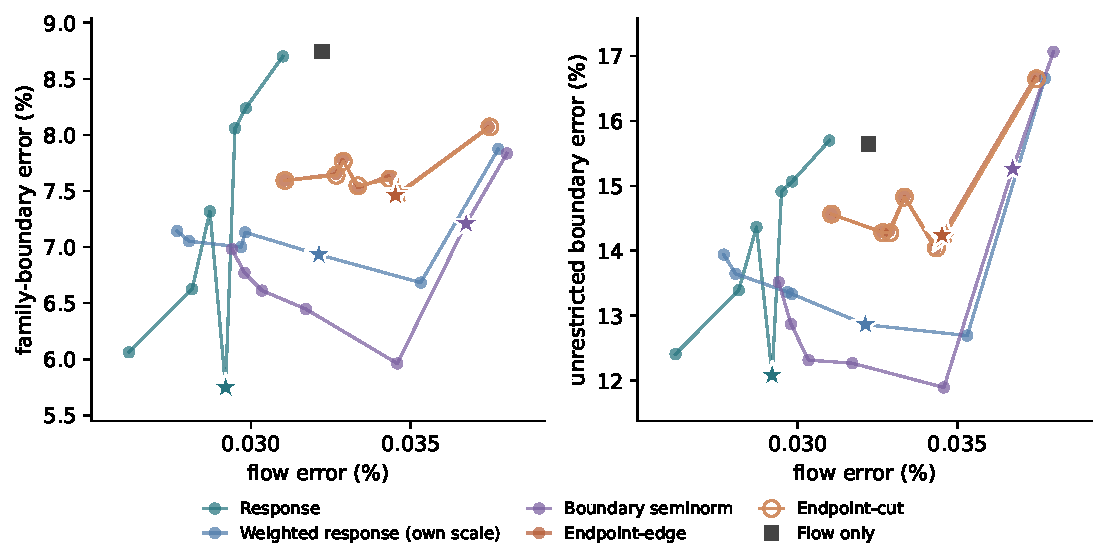
\includegraphics[width=\linewidth]{../figures/fig_v110_pareto.pdf}
\caption{Explanation--flow trade-off of the six supervision objectives
across the weight grid, on the 96 Sioux Falls test paths. Each point
is one (objective, weight) configuration: median flow error against
median family-boundary error (left) and unrestricted boundary error
(right); the validation-selected weight of each objective is starred.
Response supervision sweeps the efficient frontier in both panels,
interpolating between flow-only behavior and the lowest boundary
error. Under its own scale normalization the weighted-response
objective tracks the same band across the low-to-mid weights; only the
largest weight violates the validation flow-accuracy constraint and
selects the initial checkpoint. The boundary-seminorm objective
reaches its best errors only at unselected intermediate weights, and
the endpoint objectives (nearly coincident; the cut term is a
fixed-ratio minor addition) trace interior curves.}
\label{fig:v109pareto}
\end{figure}

\subsection{Group-level uncertainty for the 96-path comparison}\label{supp:learningdetail}
\begin{table}[pos=htbp]\centering\footnotesize
\caption{Per-seed medians of path-level values on the 96 paths and
path-level improvement counts (response vs.\ flow supervision).}\label{tab:fiveseed}
\setlength{\tabcolsep}{4.5pt}
\begin{tabular*}{\tblwidth}{@{\extracolsep{\fill}}r cc cc cc}
\toprule
& \multicolumn{2}{c}{Column (\%)} & \multicolumn{2}{c}{Geometric (\%)} & \multicolumn{2}{c}{Improved paths}\\
\cmidrule(lr){2-3}\cmidrule(lr){4-5}\cmidrule(lr){6-7}
Seed & flow & resp. & flow & resp. & col. & geo.\\
\midrule
0 & 19.55 & 15.93 & 8.40 & 5.67 & 85/96 & 84/96\\
1 & 15.66 & 12.44 & 7.07 & 4.57 & 80/96 & 84/96\\
2 & 22.81 & 14.91 & 9.08 & 6.52 & 88/96 & 89/96\\
3 & 22.33 & 14.95 & 7.40 & 5.98 & 87/96 & 84/96\\
4 & 16.65 & 12.02 & 6.57 & 4.23 & 87/96 & 91/96\\
\bottomrule\end{tabular*}\end{table}

Path-level bootstrap intervals for the paired median differences
(10,000 resamples; column error / family-boundary error, in percentage
points): single-query group $[-4.90,-2.95]$ / $[-1.99,-0.88]$
improving 24/24 and 23/24 paths; two-query group $[-6.48,-4.31]$ /
$[-3.15,-1.52]$, 22/24 and 21/24; three-query group $[-9.26,-3.36]$ /
$[-4.11,-1.36]$, 22/24 and 22/24; six-query group $[-8.59,-5.22]$ /
$[-3.86,-1.73]$, 24/24 and 24/24. Leave-one-path-out medians of the
paired column difference vary within $[-5.11,-4.94]$ and of the paired
family-boundary difference within $[-2.11,-2.00]$, so no single path
carries the result. The system-contribution difference has median
$+0.45$ percentage points with interval $[0.01,0.74]$, improving 39 of
96 paths, while both methods retain system errors below $3.5\%$
(medians $2.52\%$ and $3.13\%$).

The incremental-flow error of Table~\ref{tab:pathtable} uses the same
aggregation as the other columns (medians of path-level values, active
queries and seeds averaged within each path), and the reference
increments are well conditioned: the smallest reference increment norm
is $45$ veh/h on Sioux Falls and $508$ veh/h on Anaheim against medians
of $258$ and $1{,}672$. Response supervision therefore improves not
only the boundary attributions but also the incremental flow response
from which they are integrated, while the total-flow errors stay near
$0.03\%$ because total flows are dominated by the unchanged background.

Figure~\ref{fig:v109convergence} reports the validation curves behind
the extended-budget comparison of Section~\ref{sec:pairresults}: on
both networks the seed-median response curve stays below the flow curve
at every validation point, and both continue to decrease at the
3{,}600-update cap.
\begin{figure}[t]
\centering
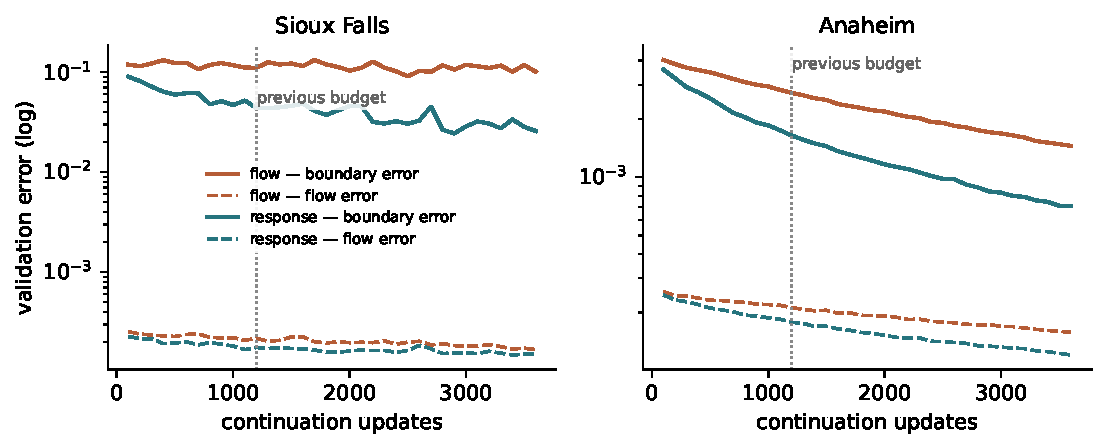
\includegraphics[width=\linewidth]{../figures/fig_v109_convergence.pdf}
\caption{Validation convergence under the extended continuation budget
(seed-median validation boundary error, solid, and relative flow
error, dashed; log scale): Sioux Falls (left) and Anaheim (right),
flow-only (ochre) versus response supervision (teal). The dotted line
marks the 1{,}200-update budget of the main comparison; both
objectives keep improving beyond it, and the response curves stay
below the corresponding flow curves throughout.}\label{fig:v109convergence}
\end{figure}

\subsection{Unrestricted and integrated-bound errors by group}\label{supp:boundchain}
Table~\ref{tab:boundchain96} completes Table~\ref{tab:pathtable} with
the unrestricted and integrated-bound columns of
Eq.~\eqref{eq:localboundarybound}, as percentages of the reference
column's boundary seminorm; the geometric and unrestricted columns use
different denominators and are not one inequality, and the bound chain
$\mathcal K_j(e_j)\le B_j$ holds in absolute units for the shared
quadrature (Section~\ref{sec:pairresults}).
\begin{table}[pos=htbp]\centering\footnotesize
\caption{Unrestricted (exact $\mathcal K_j(e_j)$ over all separating
regions) and bound (integrated bound of
Eq.~\eqref{eq:localboundarybound}) errors, medians of path-level values
on the 96 test paths, as percentages of the reference column's
boundary seminorm.}\label{tab:boundchain96}
\begin{tabular}{rcc cc}\toprule
& \multicolumn{2}{c}{Unrestricted (\%)} & \multicolumn{2}{c}{Bound (\%)}\\
\cmidrule(lr){2-3}\cmidrule(lr){4-5}
Active & flow & resp. & flow & resp.\\\midrule
1 & 4.54 & 2.95 & 4.62 & 3.00\\
2 & 15.48 & 12.65 & 15.67 & 12.80\\
3 & 16.36 & 12.39 & 16.70 & 12.81\\
6 & 19.43 & 12.28 & 20.61 & 13.48\\
\midrule
All 96 & 15.65 & 12.08 & 16.34 & 12.83\\
\bottomrule\end{tabular}\end{table}

\subsection{Complete input-stratified common-summary results}\label{sec:coverage}
Positive non-diagonal published demands are stratified by demand and directed free-flow shortest-path time using empirical tertiles, with ties kept in the lower bin. Within each of nine cells, lexicographically sorted OD indices at zero-based positions $\lfloor N/3\rfloor$ and $\lfloor2N/3\rfloor$ are retained. No attribution values enter selection. Endpoint differences identify total edge attribution, without identifying the same-state study/background response split. The two perturbation widths share every field of the selection protocol and differ only in the demand interval; their normalized errors are close for every query, so Table~\ref{tab:coveragefull} reports both in one table. Each query's common value and error follow from the tabulated range by the midpoint rule $\beta=(\phi_{\min}+\phi_{\max})/2$; absolute minima, maxima, midpoints and half-ranges for both widths, the complete normalized interval set, and the per-position boundary-value sequences behind the segmentation of Proposition~\ref{prop:segmented} accompany the result arrays in the code package.
\begin{table}[pos=htbp]\centering\footnotesize\caption{Complete geometric common summaries for the 18 input-stratified queries at both widths. Normalized error is Eq.~\eqref{eq:normerror} at $\pm10\%$ and $\pm20\%$; ranges are $[\phi_{\min},\phi_{\max}]$ at $\pm20\%$ in Sioux Falls cost units; P and M mean positive and mixed signs at $\pm20\%$.}\label{tab:coveragefull}\begin{tabular}{lrrrrl}\toprule OD & System & Range ($\pm20\%$) & Norm.\ err.\ ($\pm10\%$) & Norm.\ err.\ ($\pm20\%$) & Sign\\\midrule
(4,3) & 507.2 & [429.0, 535.0] & 9.9 & 9.9 & P\\
(12,3) & 337.2 & [330.7, 340.2] & 1.4 & 1.4 & P\\
(6,1) & 2360.6 & [658.3, 2290.4] & 35.6 & 35.6 & P\\
(15,6) & 9390.2 & [415.4, 4433.5] & 45.3 & 45.3 & P\\
(6,21) & 4577.8 & [-3.4, 2349.4] & 50.1 & 50.1 & M\\
(18,14) & 3422.3 & [150.8, 1929.7] & 46.1 & 46.1 & P\\
(8,4) & 25097.5 & [1270.7, 15741.3] & 46.0 & 46.0 & P\\
(19,8) & 16939.7 & [733.2, 7266.4] & 45.0 & 45.0 & P\\
(11,6) & 6165.9 & [1236.4, 6106.4] & 39.9 & 39.9 & P\\
(16,2) & 17763.1 & [896.3, 9628.6] & 45.3 & 45.3 & P\\
(8,21) & 7605.5 & [752.6, 4214.1] & 41.1 & 41.1 & P\\
(14,8) & 17445.3 & [890.3, 7527.1] & 44.1 & 44.1 & P\\
(11,15) & 47925.5 & [17628.9, 27737.8] & 18.2 & 18.2 & P\\
(17,9) & 24040.9 & [5482.3, 18519.3] & 35.2 & 35.2 & P\\
(10,12) & 55214.5 & [9822.4, 33248.6] & 35.2 & 35.2 & P\\
(13,10) & 54411.9 & [2918.8, 31345.2] & 45.3 & 45.3 & P\\
(1,10) & 33917.2 & [2182.9, 20856.4] & 44.8 & 44.8 & P\\
(10,1) & 34264.5 & [2182.7, 21039.5] & 44.8 & 44.8 & P\\
\bottomrule\end{tabular}\end{table}

\begin{table}[pos=htbp]\centering\footnotesize
\caption{Tolerance sensitivity of the reported summaries, within
fixed projection directions (the input-stratified selection experiment for Sioux Falls, 18 queries
per level, 36 normals with duplicate chains removed; the Anaheim ordered-family experiment for
Anaheim, six single-direction queries). Single: number of queries whose
whole family admits one common value at the stated tolerance;
segments: median per-direction count on Sioux Falls at load levels
$0.7/1.0/1.3$ (maximum over directions in parentheses) or per-query
range on Anaheim; compression: $1-$segments/regions, median per
direction (Sioux Falls) or per query (Anaheim).}\label{tab:tolerance}
\begin{tabular}{rrrrr}\toprule
Tolerance $\tau$ & Sioux single ($0.7/1.0/1.3$) & Sioux med.\ seg./dir. & Anaheim segments & Anaheim compression\\\midrule
$2.5\%$ & $2/1/0$ & $4.0\,(10)/4.5\,(12)/5.5\,(13)$ & $6$--$21$ & $91.5\%$\\
$5\%$ & $2/1/0$ & $3.0\,(7)/4.0\,(8)/4.5\,(10)$ & $4$--$14$ & $93.8\%$\\
$7.5\%$ & $2/1/1$ & $2.0\,(7)/3.0\,(8)/3.0\,(8)$ & $3$--$12$ & $95.5\%$\\
$10\%$ & $2/2/1$ & $2.0\,(6)/2.0\,(6)/2.5\,(7)$ & $3$--$12$ & $96.4\%$\\
\bottomrule\end{tabular}\end{table}

\paragraph{Tolerance rule and small-magnitude detail.}\label{supp:tolerance}
The absolute rule is absolute: $\epsilon_j=5\%$ of the family's largest
attribution magnitude, so it permits errors much larger than $5\%$ of the
small attributions. The mixed rule
$|\hat a_i-a_i|\le\epsilon_{\mathrm{abs}}+\tau|a_i|$ keeps relative
control at small magnitudes; a candidate segment admits a common
representative iff $\max_{i\in I}(a_i-t_i)\le\min_{i\in I}(a_i+t_i)$
with $t_i=\epsilon_{\mathrm{abs}}+\tau|a_i|$, feasibility is inherited
by subintervals, and the same greedy returns the minimum count. On
Anaheim, at the absolute rule the worst relative error at
small-magnitude positions (attributions below $10\%$ of the family
maximum) has median $0.55$ and maximum $0.94$; the mixed rule with
$\epsilon_{\mathrm{abs}}=1\%$ of the family maximum and $\tau=10\%$
lowers these to $0.28$ and $0.45$ while the median segment count rises
from 10 to 12 (per-query range 6--17), i.e.\ the compression is
essentially retained and the detail at small-magnitude positions
doubles in accuracy. Enlarging the relative part of the absolute
$5\%$ absolute rule without shrinking the absolute floor
($\epsilon_{\mathrm{abs}}=5\%$, $\tau\ge5\%$) instead reduces
segment counts by merging large-magnitude runs while the
small-position error worsens --- confirming that the absolute floor,
not the relative part, controls the small-magnitude detail.

\paragraph{Load-level protocol and node-imbalance diagnostics.}
The load-level experiment solves one equilibrium per level ($0.7$,
$1.0$, $1.3$ times the published demands), the focal query moving
alone over $\pm20\%$ under the identical geometric family. Across the
54 query--level pairs, the node-imbalance norm $\norm{d_j}_2$ of
Eq.~\eqref{eq:endpointd} rises $13.2$-fold from the light to the
heavy baseline (medians $1196.4$ to $15763.3$), tracks the
geometric-family spread and the unrestricted range $S_j$ with rank
correlation $0.99$, and the realized ratio $S_j/\norm{d_j}_2$ has
median $2.53$ against the Cauchy--Schwarz bound $\sqrt{n-2}=4.69$ of
Eq.~\eqref{eq:cutgap} --- mechanism-consistent readings of
Eq.~\eqref{eq:cutspread} in which the load levels change realized
weights, responses and demand increments together.

\subsection{Computational protocol for alternative attribution orders}\label{supp:pathrobust}
Each of the 22 alternative orders of Section~\ref{subsec:pathrobust}
changes the six study ODs one at a time (41 quadrature states per
segment, identical solver tolerance, endpoints and boundary family as
the straight-line run; canonical order, reverse order, and twenty
permutations under seed 20261031). Numerical checks: straight-line columns
reproduce the stored reference arrays to $1.7\times10^{-15}$ relative; every
order's endpoint equilibria match the straight-line endpoints to
$6.1\times10^{-9}$; the path-independent total outcome change
reproduces to $1.5\times10^{-7}$ relative. Each order's record stores
the attribution column, family range, common summary and normalized
error, sign-crossing flag, maximum profile deviation against the
straight-line attributions, and mechanism components at the fixed regions
$U_-$ (arrays in the code package). The dominant mechanism at $U_-$
coincides with the straight line's on all 22 orders for each of the
three mechanism-tracked queries.

\begin{table}[t]\centering\footnotesize
\caption{Attribution-path robustness on the responsive-background six-query
protocol: straight-line joint path versus 22 one-at-a-time orders
(canonical, reverse, 20 seeded permutations). $C_j$ range: minimum and
maximum over the orders; deviation relative to the straight-line
value. $\varepsilon$ shift: median normalized common-summary error
over the orders against the straight-line value. Sign: orders whose
family range keeps the straight-line sign-crossing status; mechanism:
orders whose largest-magnitude component at $U_-$ matches the straight
line's.}\label{tab:pathrobust}
\begin{tabular}{lrrrrr}\toprule
OD & $C_j$ range & Max $|C_j|$ dev. & $\varepsilon$ shift & Sign & Mechanism\\\midrule
$(7,18)$ & $[666.5,\ 678.4]$ & $1.0\%$ & $4.3\%\to4.3\%$ & $22/22$ & ---\\
$(1,19)$ & $[48{,}451.9,\ 51{,}817.7]$ & $3.4\%$ & $56.3\%\to56.4\%$ & $22/22$ & $22/22$\\
$(4,5)$ & $[2{,}780.8,\ 2{,}911.4]$ & $3.0\%$ & $8.2\%\to8.2\%$ & $22/22$ & ---\\
$(1,15)$ & $[75{,}306.6,\ 79{,}553.2]$ & $2.8\%$ & $49.3\%\to49.3\%$ & $22/22$ & $22/22$\\
$(6,8)$ & $[72{,}157.8,\ 75{,}713.7]$ & $2.4\%$ & $15.4\%\to15.5\%$ & $22/22$ & ---\\
$(7,12)$ & $[117{,}367.2,\ 117{,}573.5]$ & $0.1\%$ & $52.6\%\to52.5\%$ & $22/22$ & $22/22$\\
\bottomrule\end{tabular}\end{table}

\subsection{Anaheim learned-assignment protocol}\label{app:anaheimlearning}
The Anaheim experiment mirrors the Sioux Falls protocol in structure;
differences are stated here once. The study queries are the six largest
published OD demands of Section~\ref{sec:anaheim}; all remaining
positive demands are fixed with endogenous route choice over the same
ten-path centroid-restricted structure. The model is the conservative
parameterization of Eq.~\eqref{eq:consparam} with $K=1{,}406$ OD
softmaxes over $P=14{,}060$ paths and $m=914$ link outputs; the input
is the six-dimensional study demand vector. Reference labels: 1{,}000
flow states ($q\sim U(0.65,1.3)\,q_{\mathrm{base}}$; 800 train, 200
validation), 480 derivative centers (384 train, 96 validation) with
equilibrium sensitivities of the six study columns, and 48 test demand
paths (twelve per active-query group $k\in\{1,2,3,6\}$, mixed and same
signs, generation rule identical to the Sioux Falls test paths under a
fresh seed) solved at a 21-state quadrature with sensitivities at every
state. Training: stage~A pretrains flow-only from scratch for up to
4{,}000 steps (Adam, learning rate $3\times10^{-3}$, batch 128,
per-link scaled MSE, best-validation selection every 50 steps); stage~B
continues for 1{,}200 steps with the method objective exactly as in
the Sioux Falls protocol (learning rate $3\times10^{-5}$, batch 32
flow samples plus 8 derivative centers, rotation over the six study
columns), methods \emph{flow} and \emph{response}, five seeds.
Validation: flow relative error on the 200 held-out flow states;
$K$-MSE, the boundary-seminorm of the weighted response discrepancy
normalized per query, on the 96 held-out centers. Selection: minimum
validation $K$-MSE among states with validation flow error at most
1.1 times the stage-A checkpoint, else minimum flow error; test
paths enter neither training nor selection. Selected checkpoints
cluster at the training cap, as in Sioux Falls, so the operating
point is budget-limited rather than validation-plateaued; the
extended-budget replication below triples the cap under the identical
rule. Numerical checks: conservation of every reference state (study
plus background supply) holds to $9.1\times10^{-12}$ vehicle-units;
reference-column completeness relative to the endpoint outcome change
is at most $1.2\times10^{-5}$; the total error of every reported
summary stays within its budget. Costs: reference data 2{,}488
equilibrium solves with sensitivities ($\approx$35\,s per state
single-threaded, parallelized over twelve workers), pretraining
$\approx$40\,minutes per seed, fine-tuning $\approx$5--9\,minutes per
(method, seed).

\paragraph{Extended budget.}
The convergence check of Section~\ref{sec:pairresults} repeats the
stage-B continuation for both methods and five seeds with the budget
tripled to 3{,}600 updates: identical initialization, learning rate,
batches, label sets, validation cadence and selection rule, and the
same test paths for the final report. The extension is an exact
continuation of the shared protocol on Sioux Falls, where the
3{,}600-update runs repeat the 1{,}200-update stage with the same
initialization and minibatch sequence. Every Anaheim run selects beyond
the original cap (all five response seeds at 3{,}600 updates); the
3{,}600-update fine-tuning takes $\approx$30--105 minutes per
(method, seed) single-threaded on Anaheim and $\approx$4--6 minutes
per run on Sioux Falls.


\end{document}
